\documentclass[10pt, a4paper]{article}
\usepackage[utf8]{inputenc}
\usepackage[ngerman]{babel}
\usepackage{amsmath}
\usepackage{amsfonts}
\usepackage{amssymb}
\usepackage{graphicx}
\usepackage{tabularx}
\usepackage[autostyle]{csquotes}
\usepackage{acronym}
\usepackage{multirow}
\usepackage{siunitx}
\usepackage[
	backend=bibtex,
	style=ieee,
	sortlocale=ch_DE,
	sorting=none,
	natbib=true,
	url=true, 
	doi=true,
	eprint=false
]{biblatex}
\usepackage{float}
\usepackage{listings}
\usepackage{longtable}
\usepackage{titlesec}
\newcommand{\sectionbreak}{\clearpage}
\restylefloat{table}
\addbibresource{ba_meierto3_mekesyac.bib}
\usepackage{hyperref}
\hypersetup{
	colorlinks,
	citecolor=black,
	filecolor=black,
	linkcolor=black,
	urlcolor=black
}

\makeatletter

\renewcommand{\lstlistingname}{Listingsverzeichnis}

\renewcommand\listoftables{%
	\subsection{\listtablename}%
	\@mkboth{\MakeUppercase\listtablename}%
	{\MakeUppercase\listtablename}%
	\@starttoc{lot}%
}

\renewcommand\listoffigures{%
	\subsection{\listfigurename}%
	\@mkboth{\MakeUppercase\listfigurename}%
	{\MakeUppercase\listfigurename}%
	\@starttoc{lof}%
}

\renewcommand\lstlistoflistings{%
	\subsection{\lstlistingname}%
	\@mkboth{\MakeUppercase\lstlistingname}%
	{\MakeUppercase\lstlistingname}%
	\@starttoc{lol}%
}
\makeatother

\title{Fehlervorhersage in Java-Code mittels Machine Learning}
\author{Tobias Meier (meierto3), Yacine Mekesser (mekesyac)}
\date{10.06.16}
\begin{document}
	
\hyphenation{
	Soft-ware-ent-wick-lung
	Dem-ent-sprech-end
	PROMISE
	Fea-tu-re
	Ver-fah-ren
	Is-sue
	Track-ing
	Sys-tem-en
	Git-Hub
	Re-posi-tory
	Re-posi-tories
}

\tableofcontents
\pagebreak

\section{Einleitung}
% alternative/zusätzliche einleitung: Grosse firmen schreiben super viel code, mit agilen methoden ändert sich die code base ständig. um fehlerfreiheit zu garantieren, muss man automatisieren.

In vielen Bereichen unseres Lebens sind softwaregestützte Systeme anzutreffen. Nicht nur die Menge an Softwareprojekten, sondern auch deren Komplexität nimmt stetig zu. Damit steigt sowohl die Wahrscheinlichkeit als auch die Auswirkung von Softwarefehlern. Ausserdem kämpfen viele Firmen mit einem grossen Umfang an Code, der sich gerade mit agilen Entwicklungsmethoden dauernd verändert. Damit wird die Qualitätskontrolle einer solchen Codebasis enorm schwierig.

Die Motivation dieser Bachelorarbeit besteht darin, die Grundlage für ein Tool zu schaffen, welches in Zukunft dazu in der Lage ist, Bugs im Programmcode vorherzusagen. Damit könnten Entwickler Fehler schneller finden und Projektmanager ihre Ressourcen effizienter auf kritische Komponenten einplanen.

Diese Arbeit befasst sich mit statischer Java-Code- und Metadaten-Analyse zur Vorhersage von Softwarefehlern. Im Gegensatz zu den meisten bestehenden Fehleranalyseprodukten versuchen wir, eine Fehlervorhersage mittels  \ac{ML} zu realisieren. Ausserdem wird untersucht, ob Konzepte, die normalerweise in der Textanalyse verwendet werden, auch in der Analyse von Source Code anwendbar sind.

Als Grundlage der Fehlervorhersagen dienen verschiedene Metriken. Diese werden aus dem bestehenden Source Code eines Softwareprojekts, dessen Versionsverwaltung und Issue-Tracking berechnet. Aus den daraus generierten Features wird dann ein Trainingsdatensatz gebildet. Damit kann ein \ac{ML}-Modell trainiert werden, sodass es anschliessend möglichst zuverlässige Vorhersagen über neue Datensätze treffen kann.

\subsection{Übersicht}
Der Einsatz von \ac{ML} erfordert Trainings- und Testdaten. Die Arbeit beschränkt sich deshalb nicht nur auf das Feature Design und das Implementieren eines \ac{ML}-Modells, sondern befasst sich auch mit dem Data Mining. Dafür wurde ein Repository Mining Tool implementiert, welches den ersten Teil der Arbeit bildet.

Das anschliessende Generieren der Features über den Source Code und die gesammelten Projektmetadaten erledigt ein Feature Extractor.

Am Ende werden die generierten Features von einer \ac{ML}-Komponente zum Trainieren eines Modells verwendet. Als Trainings- und Testdaten dienen Dateiversionen aus verschiedenen Zeiträumen eines beliebigen Java-Projekts.

\subsection{Nötiges Vorwissen}
Erfahrung im Umgang mit Versionierungs- und Issue-Tracking-Systemen ist von Vorteil. Dem Leser sollten die Begriffe Dateiversion, ``Commit'', ``Bug'' und ``Enhancement'' im Bezug auf solche Systeme bekannt sein. Mögliche Einstiegspunkte in dieses Thema sind die GitHub Guides \cite{githubguides} sowie die Dokumentation von Git \cite{gitdocumentation}.

Rudimentäre Kenntnisse von statischer Code-Analyse und deren gängigsten Metriken sind nicht zwingend notwendig, aber zweckdienlich. Ebenfalls von Vorteil ist statistisches Vorwissen.

Grundlegende Kenntnisse im Themenfeld ``\acl{ML}'' sind für das Verständnis unabdingbar. Für einen umfassenden Einstieg in \ac{ML} empfehlen wir den Coursera-Kurs \emph{Machine Learning} von Andrew Ng \cite{ngcoursera}, welcher auch uns beim Einarbeiten in dieses umfassende Thema geholfen hat.

Details zu den genutzten \ac{ML}-Algorithmen werden im Kapitel \ref{sec:regressionmodels} beschrieben. Im Kapitel \ref{sec:regressionmetrics} wird auf die verwendeten Regressions-Metriken grob eingegangen.

\subsection{Ausgangslage}
% Nennt bestehende Arbeiten/Literatur zum Thema -> Literaturrecherche
% Stand der Technik: Bisherige Lösungen des Problems und deren Grenzen
%Der Einsatz von Machine Learning um Softwarefehler vorherzusagen ist üblich. 

%Hier ein paar grundlegende Beispiele 

Fehlervorhersage hat in der Softwareentwicklung einen grossen Stellenwert. Dementsprechend ist sie ein grosses Gebiet, in dem bereits Arbeiten und Produkte zu Dutzenden Ansätzen bestehen. Im Folgenden soll deshalb der Kontext dieser Arbeit erläutert werden. Es werden zunächst einige bestehende Code-Analyse-Lösungen aufgezeigt. Anschliessend wird auf die Erkenntnisse unserer Literaturrecherche zu den Themen \ac{ML} und Fehlervorhersage eingegangen.

\subsubsection{Statische und dynamische Code-Analyse}
Statische Code-Analyse (engl. static program analysis, manchmal auch als \emph{linter} bezeichnet) ist eine typische Analyseform für Computersoftware, welche versucht, Fehler oder qualitative Mängel (``Code Smell'') in Programmcode zu finden, ohne dass das Programm dafür ausgeführt werden muss. Dafür wird meistens direkt der Source Code analysiert, manchmal aber auch der Maschinencode oder die erzeugte Intermediate Language.

Man kann die statische Code-Analyse den White-Box-Testverfahren zuordnen, da der Source Code dazu benötigt wird. Je nach Tool variiert die Analysetiefe und der Detailgrad, manche markieren bloss syntaktische Fehler im Editor, andere versuchen z. B. die Korrektheit des Codes mittels formaler Methoden mathematisch zu beweisen. Insbesondere für Dienstleister mit hohen Anforderungen an Sicherheit, wie z. B. Banken, Verkehrsbetrieben oder Kernkraftwerken, ist ein hohes Mass an Fehlerfreiheit nötig.

Im Unterschied zur statischen Code-Analyse erfordert die dynamische Code-Analyse die Ausführung von Programme auf einem realen oder virtuellen Prozessor, um sie zu analysieren. Beispiele für dynamische Code-Analyse-Tools sind: \emph{Valgrind} \cite{valgrind}, ein umfassendes Dynamic-Analysis-Framework für C, \emph{Cobertura} \cite{cobertura}, ein Code-Coverage-Utility für Java, oder ferner \emph{American Fuzzy Lop} \cite{amf}, ein security-orientiertes, leistungfähiges Fuzzing-Tool.

Für Java gibt es eine Vielzahl von statischen Code-Analyse-Tools: Zum Beispiel sucht \emph{FindBugs} \cite{findbugs} den Java-Bytecode nach Fehlermustern ab, \emph{Checkstyle} \cite{checkstyle} prüft das Einhalten von Coding Standards und \emph{PMD} \cite{pmd} versucht regelbasiert ineffizienten Code aufzuspüren. Ebenfalls erwähnenswert sind \emph{Lint} \cite{lint} für C wegen seiner historischen Relevanz und \emph{Code Climate} \cite{codeclimate}, da es nicht nur multilingual ist, sondern auch durch seinen \ac{PaaS} auffällt.

Diese Arbeit nutzt ausschliesslich den Source Code, Informationen des Issue-Trackings und der Versionsverwaltung eines Projekts. Ein Ausführen des Codes ist nicht nötig. Deshalb lässt sie sich der statischen Code-Analyse zuordnen. 

\subsubsection{Bestehende Arbeiten} \label{sec:literatur}
Im Folgenden wird auf erwähnenswerte Arbeiten zum Thema statische Code-Analyse mit \ac{ML} eingegangen.

Einen guten Einstieg bietet ein Artikel von Chris Lewis und Rong Ou \cite{googlebugprediction}, welcher auf die Bug-Prediction von Google eingeht. Ihr Ziel ist es primär, sogenannte ``Hot-Spots'' in einer Code-Base zu finden, also Komponenten, welche speziell fehleranfällig sind, um Entwickler warnen und zur besonderen Vorsicht mahnen zu können.

Lewis und Ou weisen darauf hin, dass Rahman et al. \cite{rahman2011bugcache} einen einfachen, aber sehr wirksamen Algorithmus gefunden haben, der fast so gut performt wie komplexere Algorithmen. Die Hot-Spots werden gefunden, indem die Source-Code-Dateien nach der Anzahl vergangener Bug Fixing Commits geordnet werden. Der Nachteil dieser Methode ist, dass sie schlecht auf Änderungen reagieren kann. Auch wenn das Entwicklungsteam den Hot-Spot löst, werden diese Dateien noch immer hoch in der Liste erscheinen. Als Lösung entwickelten die Google-Ingenieure eine Formel, die bewirkt, dass ältere Commits weniger gewichtet werden. In unserer Arbeit wird dieses Mass inklusive der Zeitabhängigkeit ebenfalls aufgegriffen und als ``temporale Features'' implementiert (siehe Kapitel \ref{sec:temporalfeatures}).

Als Vorbild für weitere temporale Features, wie z. B. die Anzahl Änderungen pro Zeiteinheit, diente die Arbeit von Nagappan und Ball \cite{Nagappan2005} resp. Giger et al. \cite{Giger2011}. Beide versuchen den ``Code Churn'', also die Menge von vergangenen Änderungen an einer Komponente, für die Fehlervorhersage zu verwenden. Letztere versuchen zusätzlich, Änderungen mit einer noch feineren Granularität zu untersuchen. Damit soll unterschieden werden, ob beispielsweise nur ein Fileheader geändert wurde, welcher sicher keine Fehlerquelle sein kann, oder kritische Stellen. Die Umsetzung dieser Erkenntnis würde den Rahmen unserer Arbeit sprengen, Giger et al. haben aber gezeigt, dass die Masse sehr gute Ergebnisse liefern können.

Relevanz hat auch Barstad et al. \cite{barstad2014}. Mit ihrer Untersuchung prüften sie, ob es möglich ist, Vorhersagen mit statischer Code-Analyse und \ac{ML} über die Qualität von Source Code zu treffen. Dabei unterscheiden Barstad et al. zwischen ``well written'' und ``badly written''. Sie schlagen dazu ein Eclipse-Plugin vor und setzen auf eine Kombination aus Peer Reviews, statischer Code-Analyse und Klassifikationsmethoden. Als Trainingsdaten nutzen sie Datensätze des PROMISE-Forums \cite{promise} sowie Hand-Ins von Studenten. Das PROMISE-Forum ist eine internationale Konferenz für Predictive Models und Data Analytics im Bereich Software Engineering, welche diverse Datensätze von annotierten Daten zur Verfügung stellt \cite{promisedatasets}. Leider basieren die meisten Datensätze auf relativ altem C-Code und scheinbar sind nur die verarbeiteten Features, nicht der ursprüngliche Source Code, hinterlegt. Dadurch ist es für unsere Zwecke nicht zweckmässig. Wie die Code-Qualität der Hand-Ins bewertet wurde, wird von Barstad et al. nicht genau erläutert.

Barstad et al. setzen auf Komplexitätsmasse nach McCabe \cite{mccabe1976} und Halstead \cite{Halstead:1977:ESS:540137}, welche in unserer Arbeit ebenso miteinbezogen werden (siehe Kapitel \ref{sec:complexityfeatures}). Eine weitere Parallele findet sich darin, dass hier ebenfalls mit einer zentralen MySQL-Datenbank gearbeitet wurde. Die \ac{DB} dient als Zwischenspeicher für Features, welche anschliessend von einem Klassifikationsalgorithmus verarbeitet werden. 
Die besten Resultate erhalten sie mit einer naiven Bayes-Klassifikation. Sie erkennen damit insbesondere die ``well-written'' Methoden gut, die ``badly-written'' werden je nach Datenset höchstens zur Hälfte richtig erkannt.

Sharafat et al. \cite{Sharafat2008} versuchen, nicht Fehler, sondern generell Änderungen in einer Codebasis vorherzusagen. Die dafür eingesetzten Metriken erwiesen sich für diese Arbeit als relevant. Zu den Metriken gehören unter anderem Komplexitätsmasse, Lines of Code, Anzahl Codeobjekte etc. Ebenfalls interessant sind Dependency-Metriken, welche sie aus \acs{UML}-Diagrammen beziehen. Ein solcher Ansatz wird von unserer Arbeit aber nicht abgedeckt.

Rhaman et al. \cite{Rahman2014} vergleichen die Effektivität von statischer Code-Analyse, welche nur den Source Code analysiert, mit einer statistischen Analyse von historischen Daten der Codebasis (hier temporale Features). Dabei stellen sie fest, dass die Performance beider Ansätze je nach Problemstellung vergleichbar ist und dass in bestimmten Situationen eine Kombination die besten Resultate liefern kann. Mit unserer Arbeit verfolgen wir unter anderem ein ähnliches Ziel, nämlich ein Vergleich verschiedener Feature-Gruppen. Dies gerade auch, weil Rhaman et al. darauf hinweisen, dass ihre Befunde vermutlich nicht generalisierbar sind, da sie stark von den als Testdaten verwendeten Projekten abhängen könnten \cite{Rahman2014p10}. Es ist anzunehmen, dass dies auch für unsere Arbeit gilt.

Ebenfalls fassen Rhaman et al. eine wichtige Unterscheidung zusammen: Das Finden von Bugs (bei Rhaman et al. sog.``Static Bug-Finding'') ist eine andere Aufgabe als das Vorhersagen von Bugs (bei Rhaman et al. sog. ``Defect Prediction''). Für ersteres werden vor allem Pattern-Matching und statische Data-Flow-Analyse eingesetzt (z. B. mit den bereits beschriebenen Tools \emph{PMD} und \emph{FindBugs}). Für die Vorhersage hingegen, so glauben sie, bieten sich statistische Methoden wie \ac{ML} sehr an, was von Arisholm et al. \cite{Arisholm2010}, D'Ambros et al. \cite{DAmbros2011} und Lesmann et al. \cite{Lessmann2008} unterstützt wird.

Inspirierend für das Feature Design war für uns die Masterarbeit von Liljeson und Mohlin \cite{Liljeson831487}, welche sich ebenfalls mit Fehlervorhersage mittels \ac{ML} beschäftigt. Das Ziel von Liljeson und Mohlin war, die Effektivität der Metriken von Source Code mit denen des zugehörigen Testcodes zu vergleichen. Sie schliessen darauf, dass die Kombination von Source- und Testcode-Metriken zu schlechteren Resultaten führte als Source-Code-Metriken alleine. Der F-Score der Source-Code-Metriken betrug 0.647. Interessanterweise erzielten die Test\-co\-de-Me\-trik\-en alleine immerhin 0.578, was bemerkenswert ist, da diese nur über male Informationen über den Source Code verfügten. Dies zeigt, dass Source- und Testcode sehr eng miteinander gekoppelt sind.

Im Zuge ihrer Arbeit nutzten Liljeson und Mohlin eine Vielzahl von Code-Metriken als Features, allesamt gut beschrieben, was sich als sehr wertvoll erwiesen hat. Zu den Metriken gehören:
\begin{itemize}
	\item Lines of Code
	\item Komplexitäts- und objektorientierte Metriken
	\item Dependency-Metriken
	\item Prozessmetriken (temporale Metriken)
	\item Testmetriken
\end{itemize}
Dependency-Metriken, nach Schröter et al. \cite{Schroter:2006:PCF:1159733.1159739}, wären für uns interessant gewesen, konnten aufgrund technischer und zeitlicher Einschränkungen von uns aber nicht umgesetzt werden (vgl. Kapitel \ref{sec:morefeatures}).

Um die grosse Feature-Auswahl handhaben zu können, setzten sie auf Fe\-atu\-re-Se\-lec\-tion. Dieses Verfahren versucht, die Anzahl Features in einem Datenset so zu reduzieren, dass möglichst wenig Information verloren geht. Als Trainings- und Testdaten verwendeten Liljeson und Mohlin ein einziges internes Projekt ihres Industriepartners \emph{Ericsson}. Um die Metriken zu extrahieren, nutzten sie grösstenteils ein selbst entwickeltes Toolset. Für die \ac{ML}-Komponente wurden diverse Algorithmen verwendet, darunter Naive Bayes, AdaBoost, Bagging und Random Forest, wobei letzterer am Besten performte. Es sei aber darauf hingewiesen, dass Liljeson und Mohlin ein Klassifikationsproblem untersuchten. Unsere Arbeit beschränkt sich hingegen auf ein Regressionsproblem.

Ein Ziel unserer Arbeit war, typische Metriken aus der Textanalyse für die Fehlervorhersage einzusetzen. Insbesondere N-Grams bewerteten wir als vielversprechend. Tatsächlich fanden sich keine Arbeiten, welche dies bereits versucht hätten.

In seiner Masterarbeit implementierte Devin Chollack \cite{chollak2015} eine Lösung, welche Softwarefehler mittels N-Grams lokalisieren soll. Dabei setzte er aber kein klassisches \ac{ML} ein, sondern nutzte N-Grams, um automatisch eine Regelsammlung aus dem Kontrollfluss eines Programms zu generieren. Neuer Programmcode kann dann auf Verstösse dieser Regeln überprüft werden. Folgt z. B. in vielen Fällen auf einen Methodenaufruf \(A\) entweder ein Aufruf \(B\) oder \(C\), dann wird dies als Regel \(A(B|C)\) erkannt. Eine Abfolge \(ABD\) würde dann als Fehler gewertet werden. Wie effektiv dieser Ansatz ist, lässt sich anhand dieser Arbeit schlecht bewerten, da die verwendete Datenbasis nicht umfassend annotiert wurde.

Einen ähnlichen, regelbasierten Ansatz behandelten Nessa et al. \cite{Nessa}. Ausserdem finden sich einige Arbeiten wie die von Choi et al. \cite{Choi2011} und Zhang et al. \cite{Zhang2007}, welche N-Grams einsetzen, um Schadsoftware zu finden. Choi et al. bearbeiten aber nur kleinere Code-Abschnitte, wie sie z. B. in Injection- oder XSS-Angriffen eingesetzt werden. Diese sind schwierig mit Java-Klassen zu vergleichen. Zhang et al. analysieren kompilierte Executables, was ebenfalls nicht mit unserer Arbeit vergleichbar ist.

Auf der Suche nach geeigneten Trainings- und Testdaten stiessen wir auf die \ac{MSR}-Konferenz \cite{msr2016}. Diese befasst sich mit dem Analysieren der vielen Daten, die ein Softwarerepository bietet. Damit sollen interessante und nützliche Informationen über Softwaresysteme und -projekte gefunden werden. Das gesetzte Ziel der \ac{MSR} für das Jahr 2016 befasst sich mit dem Repository Mining von grossen Versionsverwaltungssystemen wie GitHub \cite{githubhomepage} und SourceForge \cite{sourceforgehomepage}. Dies scheint vielversprechend zu sein und die Resultate könnten in eine zukünftige Arbeit über Fehlervorhersage einfliessen.

Dyer et al. \cite{Dyer:2015:BUS:2852270.2803171} beschreiben in ihrer Arbeit die Sprache \emph{Boa} \cite{boahomepage}, welche als Abfragesprache für die gesammelten Repository-Daten der \emph{\ac{MSR} 2016} dient. Die Infrastruktur basiert auf \emph{Hadoop}, Anfragen werden direkt in der Cloud bearbeitet. Der Einsatz von Hadoop erwies sich für unsere Arbeit aber als zu aufwändig. Des Weiteren schien die \emph{Boa} Umgebung sehr komplex und Issue-Tracking-Daten (Enhancements oder Bugs) sind in der Datensammlung nicht vorhanden.

Andere Code Repositories, wie zum Beispiel das Software Artifact Infrastructure Repository \cite{softwareartifactinfrastructurerepo}, beinhalten eine Menge an kleinen Projekten mit verschiedenen Metriken. Für \ac{ML} stellt allerdings eine grosse Datenmenge die Grundvoraussetzung dar. Auch sind die in diesem Repository enthaltenen Projekte teilweise stark veraltet, weshalb sie für uns nicht in Frage gekommen sind.

\subsection{Zielsetzung}
% Formuliert das Ziel der Arbeit
% Verweist auf die offizielle Aufgabenstellung des/der Dozierenden im Anhang 
% (Pflichtenheft, Spezifikation)
% (Spezifiziert die Anforderungen an das Resultat der Arbeit)
% (Üersicht über die Arbeit: stellt die folgenden Teile der Arbeit kurz vor)
% (Angaben zum Zielpublikum: nennt das für die Arbeit vorausgesetzte Wissen)
% (Terminologie: Definiert die in der Arbeit verwendeten Begriffe)

Viele Tools zur Bug-Vorhersage verwenden ausgewählte und kategorisierte Lern- und Testdaten. Diese Arbeit soll ein Toolset bereitstellen, dass es erlaubt, Daten direkt aus Git-Repositories und Issue-Tracking-Systemen zu ziehen um anschliessend projektbezogen ein \ac{ML}-Modell zu trainieren. Neben der offensichtlichen Komponente für Machine Learning muss ein weiteres Tool zum Sammeln und Strukturieren der Projektdaten entwickelt werden.

Die Literaturrecherche (Siehe Kapitel \ref{sec:literatur}) lässt erkennen, dass es bereits viele Arbeiten über Fehlervorhersage mit Hilfe von statischen Metriken und \ac{ML} gibt. Die gängigsten Metriken sind auch in dieser Arbeit wiederzufinden. Im Unterschied zu den bestehenden Arbeiten werden zusätzlich Textanalyse-Features wie N-Grams genutzt, welche aus einer Abstraktion des Java-Source-Codes generiert werden.

Der Ansatz, statische Code- und Textanalyse-Features zu kombinieren, wurde in anderen Arbeiten bisher nicht verfolgt. Deshalb soll geprüft werden, ob diese Kombination mit dem projektbezogenen Lernen eine hinreichende Fehlervorhersage gewährleistet.

Eine weitere Zielsetzung war es, den Grundstein für folgende, auf dieser Arbeit aufbauen Projekte zu legen. Dafür soll zwar kein schlüsselfertiges Tool entwickelt werden, sondern vielmehr Prototypen, auf denen aufgebaut werden kann. Deshalb muss die Wiederverwendbarkeit der Tools gewährleistet sein. Auch das Verfahren der Datensammlung soll für zukünftige Arbeiten nützlich sein. Die Architektur der entwickelten Tools muss erweiterbar sein, so dass neue Features einfach hinzugefügt werden können.

\subsubsection{Terminologie}
Der Terminus ``Bug'' oder ``Softwarefehler'' wird in der folgenden Arbeit mehrmals verwendet. Unter einem Bug wird ein vom Benutzer erstellter Issue im Issue-Tracking-System verstanden, der als Bug oder Defekt getaggt ist.

Wird ein Softwarefehler behoben, geschieht dies in der Regel durch Anpassung des Source Codes. Der Programmierer erstellt in der Versionsverwaltung einen Commit, welcher die Änderungen beinhaltet und pusht sie anschliessend auf den Server. Der erstellte Commit enthält in der Regel eine Nachricht, welche die Anpassungen möglichst genau beschreibt. Nach üblichen Konventionen verweist der Programmierer in der Nachricht auch auf den bearbeiteten (Bug-) Issue. Diese Assoziation machen sich die Tools dieser Arbeit zunutze, um Code (Inhalt des Commits) einem Bug zuordnen zu können. Dies hat zur Folge, dass unser Toolset nur bei fachgerechtem Gebrauch des Versionsverwaltungssystems funktioniert. 

Ebenfalls anzumerken ist, dass als Bug getaggte Commits in der Regel keinen Bug-behafteten Code enthalten, sondern Code, welcher den Bug beheben soll. Deshalb kann aber davon ausgegangen werden, dass die Dateiversion \emph{vor} dem Bugfix-Commit einen Bug enthalten muss.

Ein Vorteil dieser Art der Bug-Erfassung ist, dass Bugs nur gezählt werden, wenn auch tatsächlich eine Code-Anpassung stattgefunden hat. Damit werden als Bug getaggte Issues, welche eigentlich bloss Scheinfehler waren, automatisch ignoriert.

\subsubsection{Bewertung}
Um die Qualität unseres Modells bewerten zu können, trainierten und testeten wir es mit Dateiversionen aus verschiedenen Zeitspannen eines Softwareprojekts. Das Ziel war, die Anzahl Bugfixes vorherzusagen, welche für eine Dateiversion in einer gewissen Zeitspanne (z. B. 6 Monate) auftreten.

Als Referenzwert (Baseline) dienten uns der Median und das arithmetische Mittel über die Bugfixes pro Zeitraum im Trainingsset (i. d. R. nahe bei 0), sowie einen entsprechend den Trainingsdaten gewichteten Zufallswert. 

Das Ziel war es, zu überprüfen, ob mit unseren Methoden qualitativ bessere Aussagen als mit den Baselines gemacht werden können.

\section{Theoretische Grundlagen}
% optionales kapitel
% Funktionsweise git
%% Graph-Struktur von Git
%% Was sind Merges
%% Wie werden daten gespeichert und so
%% Alles was für GtSooG wichtig ist, dort aber nicht erklärt wird.
% Unterscheidung statische/dynamische Code analyse? -> atm schon in Einleitung drin.
% ml	

\acf{ML} ist ein Gebiet der Informatik, welches sich mit selbstlernenden Programmen befasst. Anstatt einfach Beispiele auswendig zu lernen, erkennt \ac{ML} Muster und Gesetzmässigkeiten in den Lerndaten und kann diese auf unbekannte Daten anwenden. Tom Mitchell beschreibt \ac{ML} treffend:
\begin{quote}
	``A computer program is said to learn from experience E with respect to some class of tasks T and performance measure P if its performance at tasks in T, as measured by P, improves with experience E'' \cite{mitchell1997}
\end{quote}
Die Erfahrung \(E\) ist im Falle unserer Arbeit eine Sammlung von Dateiversionen eines Java-Projektes. Diese werden, nach entsprechender Verarbeitung, in zwei Datensets unterteilt: Ein Trainingsset und ein Testset. Die Aufgabe \(T\) unseres Modells ist, die kommenden Bugfixes einer Dateiversion vorherzusagen. Um diese Aufgabe zu erfüllen, trainiert das Modell mit dem Trainingsset. Die anschliessende Messung der Performance erfolgt durch das Anwenden des Modells auf das Testset. Als Mass der Performance \(P\) dienen uns verschiedene Regressionsmetriken, wie sie im Kapitel \ref{sec:regressionmetrics} beschrieben werden.

Im Folgenden werden einige grundlegende Konzepte aus den Bereichen Machine Learning und Stochastik, welche in dieser Arbeit aufgegriffen werden, genauer erläutert. Dabei wird auch darauf eingegangen, inwiefern diese für unsere Arbeit relevant sind und worauf beim Einsatz mit dem gewählten Framework \emph{Scikit-Learn} (siehe Kapitel \ref{sec:mlpipeline_design}) zu achten ist.

\subsection{Regressions-Modelle} \label{sec:regressionmodels}
Die Regressionsanalyse ist ein in der Statistik sehr häufig eingesetztes Verfahren, welches versucht, die Abhängigkeit einer abhängigen Variable von einer oder mehreren unabhängigen Variablen zu untersuchen. Dabei lassen sich die Zusammenhänge nicht nur quantitativ beschreiben, sondern es lassen sich auch Prognosen für die abhängige Variable treffen \cite{uzhregression}.

Das Ziel dieser Arbeit ist, die Anzahl in einem bestimmten Zeitraum gefundene Bugs in einer Java-Datei vorherzusagen. Das heisst, die abhängige Variable ist die Anzahl Bugs. Die unabhängigen Variablen sind die verschiedenen Features, welche wir aus dem Source Code und der File-History extrahieren.

In den folgenden Kapiteln sollen die für diese Arbeit verwendeten Modelle der Regressionsanalyse erläutert werden.

\subsubsection{Lineare Regression} \label{sec:linreg}
Eines der einfachsten Modelle der Regressionsanalyse ist die lineare Regression. Dabei wird versucht, eine lineare Kurve so auf ein Trainings-Datenset von beobachteten Werten anzupassen, dass sie möglichst nahe an den Datenpunkten verläuft (siehe z. B. Abbildung \ref{fig:linreg}).

\begin{figure}[h]
\centering
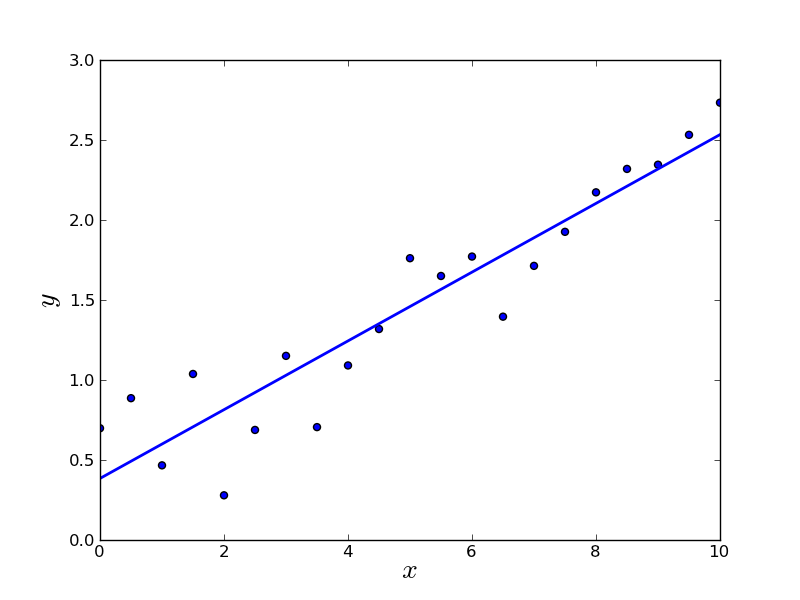
\includegraphics[width=0.7\linewidth]{resources/images/linreg}
\caption{Beispiel einer Linearen Regressionskurve. \(x\) ist die unabhängige Variable, \(y\) die abhängige \cite{netprophetlocalregression}.}
\label{fig:linreg}
\end{figure}

Dies wird in der Regel mit der Methode der kleinsten Quadrate erreicht, einem Optimierungsproblem, bei dem die Quadrate der Residuen (Differenz zwischen Beobachtung und Modell) minimiert werden \cite{sklearnlinearmodel}.
Das heisst, für ein Model mit den Koeffizienten \(\omega = (\omega_1, \dots, \omega_p)\) wird mathematisch folgendes Problem gelöst:
\[
\min_{\omega} = ||X\omega - y||_2^2
\]

An dieser Stelle soll nicht darauf eingegangen werden, mit welchen Optimierungsverfahren die idealen Koeffizienten gefunden werden können, da dies den Umfang dieser Arbeit sprengen würde. Als Beispiel eines einfachen, numerischen Verfahrens sei das Gradientenverfahren genannt \cite{gradientdescent}.

Probleme bei Linearer Regression können auftreten, wenn zwei oder mehr abhängige Variablen vollständig korrelieren. Das kann zum Beispiel auftreten, wenn ein Feature doppelt in das Datenset aufgenommen wird. Dies führt dazu, dass sich der Rang der Daten-Matrix verringert und sie nicht mehr regulär ist. In diesem Fall gibt es keine eindeutige optimale Lösung des Problems und das Modell wird sehr anfällig auf zufällige Fehler in den Trainingsdaten, was zu einer hohen Varianz führt \cite{linregmulticollinearity}.

In dieser Arbeit ist dies ein Problem, da zwischen unseren Features durchaus lineare Zusammenhänge bestehen könnten: Zum Beispiel ist es anzunehmen, dass die Anzahl hinzugefügter Dateien über verschiedene Zeiträume (siehe Kapitel \ref{sec:temporalfeatures}) mehr oder weniger linear ist. Das ist einer der Gründe, warum lineare Regression für die Anwendung in dieser Arbeit ungeeignet ist. Das Modell wird aber trotzdem von der ML-Pipeline unterstützt, da es gerade für kleine Datensets vergleichsweise sehr schnell und dementsprechend nützlich für die Entwicklung der ML-Pipeline ist.

\emph{Scikit-learn} bietet lineare Regression mit der Methode der kleinsten Quadrate (ordinary least squares) als \textit{sklearn.linear\_model.LinearRegression} an. Wenn die Daten-Matrix von der Grösse \((n, p)\) ist, dann lernt das Modell mit einer Komplexität von \(
\mathcal{O}(np^2)
\), angenommen dass \(n \leq p\) \cite{sklearnlinearmodel}.

\subsubsection{Ridge Regression und polynomiale Features} \label{sec:ridgereg}
Ridge Regression adressiert einige der Probleme von einfacher Linearer Regression indem ein Regularisierungsparameter eingeführt wird.

Lineare Regression kann ausschliesslich lineare Modelle abbilden. Falls der Zusammenhang zwischen abhängigen und unabhängigen Variablen also nicht linear ist, wird ein solches Modell entsprechend schlechte Resultate liefern. Eine Möglichkeit zur Abhilfe ist, die unabhängigen Variablen so zu transformieren, dass ein lineares Modell anwendbar ist. Ein sehr effektives Verfahren ist das Anwenden von \emph{polynomialen Features}. Dabei wird der Zusammenhang zwischen abhängigen und unabhängigen Variablen als Polynom n-ten Grades dargestellt. 
So wird zum Beispiel das Modell
\[
y = \omega_0 + \omega_1 x_1 + \omega_2 x_2
\]
erweitert um polynomiale Features 2. Grades:
\[
y = \omega_0 + \omega_1 x_1 + \omega_2 x_1^2 + \omega_3 x_1 x_2 + \omega_4 x_2^2 + \omega_5 x_2
\]
Dieses Verfahren wird zum Teil auch als separate Form namens \textit{polynomial regression} behandelt. In der Implementation der ML-Pipeline dieser Arbeit wird es aber als reine Transformation des Datensets angesehen.

Durch das Multiplizieren von Features mit sich selbst und Anderen können sehr komplexe Probleme gelöst werden. Tatsächlich ist dieses Verfahren so mäch\-tig, dass es sehr anfällig auf Overfitting (Überanpassung) ist. Das bedeutet, dass das resultierende Modell zu stark auf die Trainingsdaten angepasst ist und als Konsequenz schlecht auf neue (Test-)Daten generalisiert (vgl. Abbildung \ref{fig:under_and_overfitting}).

\begin{figure}[h]
	\centering
	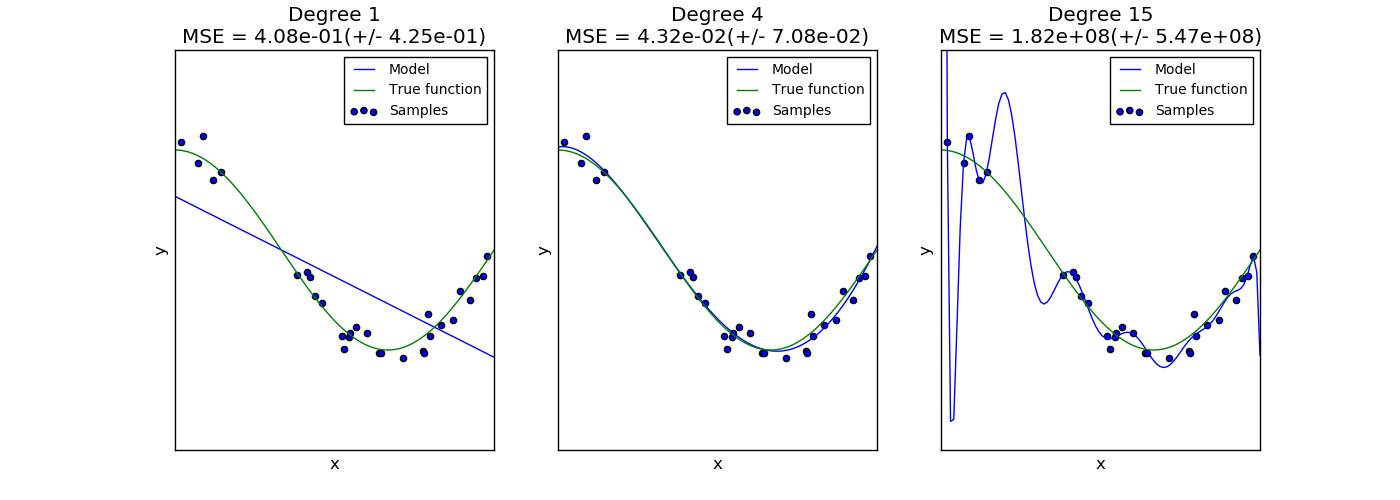
\includegraphics[width=1\linewidth]{resources/images/under_and_overfitting}
	\caption[Vergleich von Over- und Underfitting]{Links: Underfitting, das Modell bildet die Trainingsdaten schlecht ab. Mitte: Gutes Modell. Rechts: Overfitting, Modell bildet die Trainingsdaten sehr gut ab, generalisiert aber schlecht \cite{sklearnoverunderfitting}.}
	\label{fig:under_and_overfitting}
\end{figure}

Aus diesem Grund ist eine Form von Regularisierung nötig. Regularisierung ist ein einfacher mathematischer Trick, welcher die Koeffizienten stabilisiert indem ein Regularisierungsterm eingeführt wird, welcher zu hohe Koeffizienten ``bestraft''. Mit diesem Term wird das Minimierungsproblem der Linearen Regression erweitert:
\[
\min_{\omega} = ||X\omega - y||_2^2 + \alpha || \omega ||_2^2
\]
Gesteuert wird die Regularisierung über den Parameter \(\alpha \geq 0 \): Je höher \(\alpha\), desto grösser ist die ``Bestrafung'' und desto robuster werden die Koeffizienten gegenüber Kollinearität.
Diese Form von Regularisierung wird in der Literatur z.T. auch \emph{Tikhonov regularization} genannt. Der Regularisierungsparameter \(\alpha\) wird oft auch mit dem Symbol \(\lambda\) dargestellt.
\cite{ridgeregs4u, sklearnlinearmodel}

Wie ein sinnvoller Wert für \(\alpha\) bestimmt werden kann, wird im Kapitel \ref{sec:cv} beschrieben.

Ridge Regression wurde wie lineare Regression hauptsächlich in der Entwicklungsphase dieser Arbeit eingesetzt. In Kombination mit polynomialen Features wäre es zwar theoretisch geeignet, in der Praxis wird aber bei grossen Datensets die schlechte Skalierbarkeit ein Problem.

In \emph{scikit-learn} lässt sich über \textit{sklearn.linear\_model.Ridge} ein Ridge Regression Modell instanzieren. Ridge Regression hat dieselbe Komplexitätsklasse wie lineare Regression.

Eine Anmerkung zu polynomialen Features: Werden die Trainingsdaten polynomial transformiert, müssen zwingend auch die Testdaten entsprechend transformiert werden, damit das Modell anwendbar ist. Ein wesentlicher Nachteil ist, dass die Anzahl der Output-Features (und damit die Anzahl zu optimierender Koeffizienten) polynomial mit der Anzahl Features und exponentiell mit dem Grad des Polynoms ansteigt und dementsprechend die Laufzeit und den Speicherbedarf massiv erhöht. Ausserdem wird es mit polynomialen Features schwieriger, Schlüsse aus dem Modell zu ziehen, da die Koeffizienten ``verzerrt'' werden.

\subsubsection{Support Vector Regression}
\ac{SVR} ist ein auf \acp{SVM} basierendes Regressionsmodell, einem Lernalgorithmus welcher üblicherweise für Klassifizierungsprobleme eingesetzt wird.

Eine \ac{SVM} versucht Datenpunkte zu klassifizieren, indem es den Vektorraum mit einer optimalen Hyperebene (engl. hyperplane) als Klassengrenze teilt. Dies bewerkstelligt sie so, dass ein möglichst breiter Bereich (engl. margin) um die Hyperebene frei von Objekten bleibt. So wird erreicht, dass die Klassifizierung möglichst robust gegenüber Rauschen und Ausreissern bleibt. Eine solche Hyperebene wird auch ``maximum-margin hyperplane'' genannt (siehe Abbildung  \ref{fig:svr_optimal_hyperplane}).

Jeder Datenpunkt wird durch einen (Feature-)Vektor repräsentiert. Für das Finden der optimalen Hyperebene müssen nur die ihr am nächsten liegenden Datenpunkt-Vektoren, also die namensgebenden ``Support Vektoren'', be\-rück\-sich\-tigt werden. Die restlichen Vektoren sind gewissermassen verdeckt und sind nicht weiter relevant, was einen wesentlichen Vorteil bezüglich Laufzeit und Speicherbedarf darstellt \cite{svropencv}.

\begin{figure}[h]
	\centering
	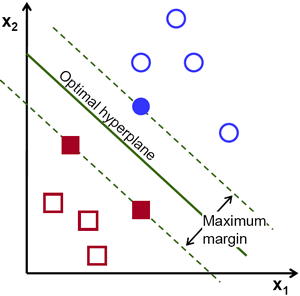
\includegraphics[width=0.4\linewidth]{resources/images/svr_optimal_hyperplane}
	\caption{Optimale Hyperebene \cite{svropencv}.}
	\label{fig:svr_optimal_hyperplane}
\end{figure}

Da Hyperebenen definitionsgemäss linear sind, lassen sich mit einer solchen \ac{SVM} nur linear trennbare Daten klassifizieren. Um \acp{SVM} auch auf linear unseparierbare Daten anzuwenden, wird der sogenannter Kernel-Trick angewendet. Dabei wird der Vektorraum in einen höherdimensionalen Raum überführt. Ziel ist es, eine Transformation zu finden, welche das Datenset linear separierbar macht. Im Falle des Beispiels in Abbildung \ref{fig:svr_2d_to_3d} wurde die Transformation \(T([x_1, x_2]) = [x_1, x_2, x_1^2 + x_2^2]\) angewandt.

\begin{figure}[h]
	\centering
	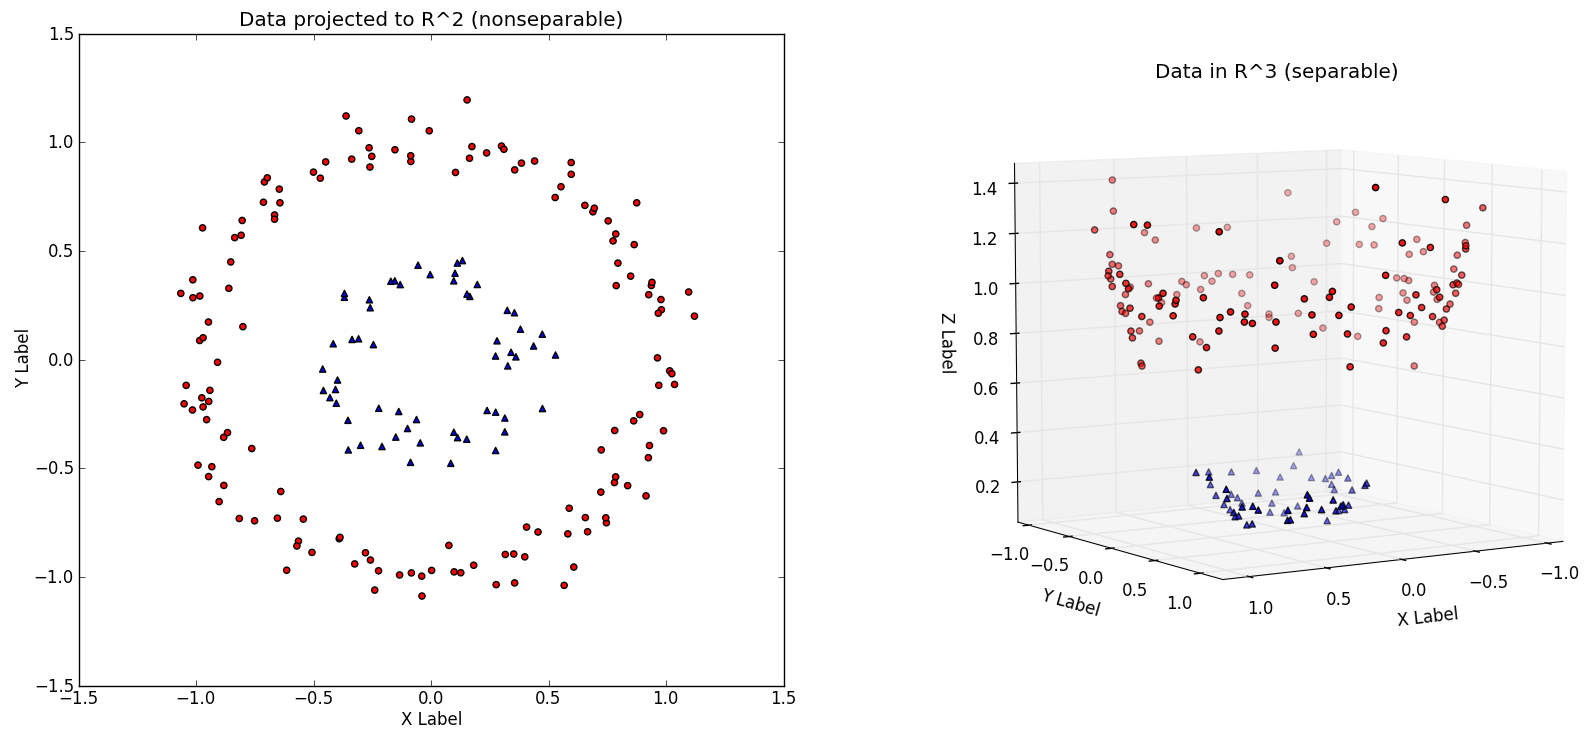
\includegraphics[width=0.7\linewidth]{resources/images/svr_2d_to_3d}
	\caption{Links: ein linear nicht separierbares Datenset in \(\mathbb{R}^2\). Rechts: Dasselbe Datenset, transformiert in einen höheren Raum ( \(\mathbb{R}^3\)): Es wird linear separierbar \cite{erickimkerneltrick}.}
	\label{fig:svr_2d_to_3d}
\end{figure}

Dies ist ein ähnlicher Ansatz wie polynomiale Features bei Ridge Regression und er führt zum selben Problem. Die Feature-Matrix wird bei hohen Dimensionen unbewältigbar gross. Es stellt sich aber heraus, dass zum Trainieren einer \ac{SVM} lediglich das paarweise Skalarprodukt \(\langle \vec{x_i}, \vec{x_j} \rangle\) der Trainingsdaten benötigt wird \cite{berkeleykerneltrick}. Nun existieren sogenannte Kernel-Funktionen, welche das Skalarprodukt zweier Vektoren in höherdimensionalen Räumen berechnen können, ohne die Vektoren explizit in diesen Raum zu transformieren. Das führt dazu, dass in der \ac{SVM} einfach alle Skalarprodukte mit der entsprechenden Kernel-Funktion ersetzt werden können. Der Algorithmus benötigt damit keinen zusätzlichen Speicher und auch der zusätzliche Rechenaufwand hält sich in Grenzen. Dieser ist lediglich abhängig von der benutzten Funktion und kann dementsprechend sehr klein sein \cite{erickimkerneltrick}.

\emph{scikit-learn} bietet folgende populäre Kernel-Funktionen an:
\begin{enumerate}
	\item \textbf{Linear}: \(\langle \vec{x_i}, \vec{x_j} \rangle\), entspricht dem normalen Skalarprodukt, also keiner speziellen Kernel-Funktion.
	\item \textbf{Polynomial Kernel}: \((\gamma \cdot \langle \vec{x_i}, \vec{x_j} \rangle + r )^d \cdot d\), wobei \(d\) der Grad des Polynoms ist und \(r\) der Bias. Diese Werte sind über den Parameter \textit{degree} respektive \textit{coef0} konfigurierbar. 
	\item \textbf{\ac{RBF} Kernel}: \(\exp(-\gamma \cdot |\vec{x_i} - \vec{x_j}|^2)\), wobei der Parameter \(\gamma\) über das Keyword \textit{gamma} konfiguriert wird.
	\item \textbf{Sigmoid Kernel}: \(\tanh(\langle \vec{x_i}, \vec{x_j} \rangle + r)\), bei dem ebenfalls die Parameter \textit{gamma} und \textit{coef0} relevant sind.
\end{enumerate}
Ausserdem lassen sich in \emph{scikit-learn} auch eigene Kernel-Funktionen definieren und einbinden. Das finden eines geeigneten Kernels für ein Problem und der passenden Parameter ist keine triviale Aufgabe, kann aber massgeblich zur Performance des Modells beitragen \cite{erickimkerneltrick, sklearnsvm}.

Neben den Parametern der Kernel-Funktionen muss auch immer noch der Regularisierungsparameter \(C > 0\) spezifiziert werden. Ein hoher Wert für \(C\) erlaubt ein komplexeres Modell, das sich stark an die Trainingsdaten anpassen kann, aber auch mehr Rechenzeit benötigt. Ein niedriger Wert hingegen glättet die Entscheidungskante und verringert damit Overfitting. \(C\) entspricht damit dem Kehrwert des \(\alpha\)-Parameters der Ridge Regression.

Da in dieser Arbeit kein Klassifizierungsproblem gelöst wird, ist \ac{SVM} ungeeignet. Deshalb verwenden wir eine Variante namens Support Vector Regression, kurz \ac{SVR}. Wie bei \acp{SVM} wird auch hier nur eine Teilmenge der Trainingsdaten verwendet. Alle beschriebenen Kernels können auch mit \ac{SVR} genutzt werden \cite{sklearnsvm}.

% Wie funktioniert SVR?

% Vorteile:
%% Effizient in hochdimensionalen Räumen (haben wir)
%% Auch effektiv, wenn die Anzahl Dimensionen grösser ist als Anzahl Samples (haben wir mit vielen Ngrams auch)
%% Memoryeffizient, da es nur ein Subset der Trainingspunkte in der Entschieundsfunktion benutzt (support vectors)
%% Vielseitig dank verschiedenen Kernel f-Funktion

% Nachteile:
%% WEnn anzahl features >> anzahl samples gibt es schlechte resultate
%% SVMs geben nicht direkt wahrscheinlichkeitsangaben, diese werden teuer via 5-fold cv berechnet

% Laufzeit hängt von K ab


\subsubsection{Cross Validation} \label{sec:cv}
Parameter wie etwa \(C\) bei \ac{SVM} oder \(\alpha\) bei Ridge Regression sind massgeblich für die Performance eines Modells. Deshalb ist die Suche nach den bestmöglichen Parametern für ein Modell eine wichtige Aufgabe.

Eine Möglichkeit, diese Suche zu automatisieren, ist das Grid-Search-Ver\-fahr\-en. Dabei wird ein Raum (oder Grid) von Parametern aufgespannt, in dem alle Kombinationen durchprobiert werden. Am Ende werden die Parameter mit den besten Resultaten ausgewählt.

\emph{scikit-learn} ermöglicht dies mit der Klasse \textit{sklearn.grid\_search.GridSearchCV}, welche mit dem Parameter \textit{param\_grid} eine Liste von Parameter-Grids entgegennimmt. Möchte man Beispielsweise ein \ac{SVM}-Modell mit einem linearen und einem \ac{RBF}-Kernel optimieren, könnte das Grid so aussehen \cite{sklearngridsearch}:

\noindent
\begin{lstlisting}[language=Python, frame=single, caption={Parameter Grid}]
param_grid = [
  {
    'C': [1, 10, 100, 1000], 
	'kernel': ['linear']
  },
  {
    'C': [1, 10, 100, 1000],
    'gamma': [0.001, 0.0001],
    'kernel': ['rbf']
  },
]
\end{lstlisting}

Mit diesen Parameterkombinationen wird dann auf dem Trainingsset gelernt. Es wäre falsch, die Qualität der Parameter mit Hilfe des Testsets zu messen, da sie sich damit auf den Testdaten optimieren würden und anschliessend keine verlässlichen Angaben zur Qualität des Modells gemacht werden könnten. Aus diesem Grund sollte aus dem Trainingsset ein sogenanntes Validationsset abgespalten werden, um die Parameter damit zu testen.

\ac{CV}, auch Kreuzvalidierung, optimiert dieses Verfahren. In der einfachsten Ausführung, der sogenannten \(k\)-Fold \ac{CV} wird das Trainingsset in \(k\) kleinere Sets aufgeteilt. Für jede der \(k\) ``Folds'' wird folgende Prozedur ausgeführt:
\begin{enumerate}
	\item Das Modell wird mit \(k-1\) der Folds trainiert;
	\item das resultierende Modell wird dann mit dem verbleibenden Teil der Daten validiert (d. h. es wird als Testset zum Berechnen des Scores verwendet) 
\end{enumerate}
Das Performance-Mass, welches von der \(k\)-Fold \ac{CV} zurückgegeben wird, ist dann der Mittelwert über alle Werte, welche in dieser Schleife berechnet wurden. Dieser Ansatz kann rechenintensiv sein, verschwendet aber nicht so viele Daten wie wenn ein separates Validationsset verwendet würde. Speziell wenn kleinere Datensets verwendet werden, ist dies ein grosser Vorteil \cite{sklearncv}.

In dieser Arbeit wird ausschliesslich \(k\)-Fold \ac{CV} verwendet, insbesondere auch weil die Anwendung mit \emph{scikit-learn} sehr einfach ist und ein separates Validationsset zusätzlichen Konfigurationsaufwand nach sich ziehen würde.

\subsection{Regressions-Metriken} \label{sec:regressionmetrics}
Um die Qualität eines Modells zu bewerten, können sich verschiedene Metriken aus der Statistik zunutze gemacht werden. Die für dieses Projekt verwendeten Metriken werden im Folgenden kurz beschrieben.

\subsubsection{Allgemeine Begriffe der Statistik}
In dieser Arbeit werden einige allgemeine Begriffe der Statistik mehrmals verwendet, die in Tabelle \ref{statisticwords} kurz erläutert werden.

\begin{table}
	\centering
	\begin{tabularx}{\textwidth}[!ht]{| c | X | X |}
		\hline
		\textbf{Symbol} & 
		\textbf{Bezeichnung} & 
		\textbf{Erklärung} \\
		\hline
		\(\mathbf{y}\) &
		Ground Truth, beobachtete y-Werte &
		Der tatsächliche Messwert \\
		\hline
		\(\mathbf{\hat{y}}\) &
		Prediction, erklärte y-Werte &
		Werte, die durch das Regressions-Modell vorhergesagt (``erklärt'') werden. \\
		\hline
		\(\mathbf{e}\) &
		Residuen, Fehler &
		Die Differenz zwischen beobachteten und erklärten Werten: \(e = y - \hat{y}\)\\
		\hline
		\(\mathbf{Var(X)}\) &
		Varianz &
		Kenngrösse der Wahrscheinlichkeitsverteilung einer Zufallsvariable. Entspricht der mittleren, quadrierten Abweichung der Werte von ihrem Durchschnitt:
		
		\(Var(X) = \frac{1}{n} \sum (X - \bar{X})^2\)\\
		\hline
	\end{tabularx}
	\caption{Relevante Begriffe der Statistik}
	\label{statisticwords}
\end{table}

\subsubsection{Varianzaufklärung}
Die Varianzaufklärung (Explained Variance) ist ein Mass dafür, wie gut ein Regressionsmodell die Streuung, also die Varianz, eines Datensatzes erklären kann.
Ist \(y\) die Ground Truth und \(\hat{y}\) die Prediction, dann berechnet sich die Varianzaufklärung aus dem Verhältnis der Varianz \(Var\) der Ground Truth und der Varianz der Residuen: 
\[
\text{explained\_variance}(y, \hat{y}) = 1 - 
\frac{Var\{y - \hat{y}\}}
{Var\{y\}}
\]
Das bestmögliche Resultat ist 1, es tritt genau dann ein, wenn die Varianz der Prediction gleichwertig zur Varianz der Ground Truth ist. Je tiefer der Wert, desto schlechter ist das Resultat bezüglich Varianz. Dabei kann die Varianzaufklärung bei beliebig grossem Unterschied auch negativ werden.

\subsubsection{Mittlerer absoluter Fehler}
Der mittlere absolute Fehler (Mean absolute Error, MAE) zeigt an, wie nahe die erklärten y-Werte an den Beobachteten liegen. Er entspricht dem Mittelwert der absoluten Residuen. Ist \(n\) die Anzahl Datensätze in \(y\), berechnet er sich folgendermassen:
\[
\text{MAE}(y, \hat{y}) = \frac{1}{n}  \sum_{i=0}^{n-1} |y_i - \hat{y}_i|
\]
Im Idealfall ist der mittlere absolute Fehler 0. Das bedeutet, dass die Prediction exakt der Ground Truth entspricht. Je höher das Resultat ausfällt, desto schlechter war die Vorhersage.

\subsubsection{Mittlerer quadrierter Fehler}
Der mittlere quadrierte Fehler (Mean squared Error, MSE) wird sehr ähnlich berechnet, wie der mittlere absolute Fehler. Anstatt des Betrags der Residuen, wird allerdings das Quadrat genommen:
\[
\text{MSE}(y, \hat{y}) = \frac{1}{n}  \sum_{i=0}^{n-1} (y_i - \hat{y}_i)^2
\]
Wie beim mittleren absoluten Fehler ist das bestmögliche Resultat 0. Höhere Fehler fallen durch die Potenzierung schwerer ins Gewicht. Für uns ist der mittlere quadrierte Fehler nicht sehr relevant, da der mittlere absolute Fehler eine nachvollziehbarere, lineare Bewertung eines Modells ermöglicht. Dieser Score wird aber bei linearer Regression im Optimierungsterm verwendet, da die Quadrierung  es dort erlaubt, einfacher abzuleiten (siehe Kapitel \ref{sec:linreg}).

\subsubsection{Median des absoluten Fehlers}
Der Median des absoluten Fehlers (Median absolute Error, MDE) ist ähnlich wie der mittlere absolute Fehler, ist aber robuster gegen Ausreisser. Er entspricht dem Median aller absoluten Residuen:
\[
\text{MDE}(y, \hat{y}) = median(|y_1 - \hat{y}_1|, \dots, |y_n - \hat{y}_n|)
\]
Hier ist ebenfalls der bestmögliche Wert 0. Zu beachten ist allerdings, dass ein Resultat von 0 nicht bedeutet, dass die Prediction exakt der Ground Truth entspricht, sondern dass mehr als die Hälfte der erklärten y-Werte der Ground Truth entsprechen. Wie beim mittleren absoluten Fehler kann das Resultat ebenfalls beliebig hoch und damit schlecht ausfallen.

\subsubsection{Bestimmtheitsmass R\textsuperscript{2}}
Das Bestimmtheitsmass (auch Determinationskoeffizient) ist der Anteil der Variation, welcher durch die lineare Regression erklärt wird. Damit dient es als wichtiges Mass der Güte der Anpassung und gibt an, ``wie gut'' ein statistisches Modell eine Menge von Beobachtungen erklären kann.
Berechnet wird das Bestimmtheitsmass aus dem Verhältnis der Variation der Residuen und der Variation von \(y\) (\(n\) ist dabei die Anzahl Datensätze in \(y\)):
\[
R^2(y, \hat{y}) = 1 - \frac
{\sum_{i=0}^{n-1} (y_i - \hat{y}_i)^2}
{\sum_{i=0}^{n-1} (y_i - \bar{y})^2}
= 1 - \frac{\text{unerklärte Variation}}{\text{Gesamtvariation}}
\]
Ein perfekter linearer Zusammenhang ergibt ein Bestimmtheitsmass von 1. Auf dem Datenset, auf das die Regressionskurve angepasst wurde, kann das Bestimmtheitsmass minimal 0 werden, was keinem linearen Zusammenhang entspricht. Auf dem Testset kann das \(R^2\) aber beliebig schlecht werden und damit auch negative Werte annehmen.

Nach Cohen \cite{cohenstatistics} lässt sich aus dem Bestimmtheitsmass zusätzlich noch die Effektstärke \(f^2\) berechnen:
\[
	f^2 = \frac{R^2}{1 - R^2}
\]
Dabei gelten nach Cohen \cite{cohenstatistics} folgende Werte, um eine Aussage über die Stärke des Effekts zu machen:
\begin{table}[H]
	\centering
	\begin{tabular}{l|l}
		\hline
		\(f^2 = 0.02\) & kleine Effektstärke \\ 
		\(f^2 = 0.15\) & mittlere Effektstärke \\ 
		\(f^2 = 0.35\) & grosse Effektstärke \\
		\hline
	\end{tabular}
	\caption{Effektstärken in \(f^2\)}
\end{table} 

Wenn man dies auf das Bestimmtheitsmass \(R^2\) zurückrechnet, ergeben sich folgende Werte  \cite{uzhregression}:

\begin{table}[H]
	\centering
	\begin{tabular}{l|l}
		\hline
		\(R^2 = 0.0196\) & kleine Effektstärke \\ 
		\(R^2 = 0.1300\) & mittlere Effektstärke \\ 
		\(R^2 = 0.2600\) & grosse Effektstärke \\
		\hline
	\end{tabular}
	\caption{Effektstärken in \(R^2\)}
\end{table}

Das heisst bei \(R^2 > 0.26\) lässt sich bereits von einer grossen Effektstärke sprechen.

\subsection{N-Grams}

N-Grams sind das Ergebnis der Zerlegung eines Textes in Fragmente. Dabei ist \emph{N} ein Platzhalter für die Anzahl zusammengehängter Fragmente. In der Textanalyse ist ein 1-Gram typischerweise ein Wort, ein 3-Gram entspricht einer Wortkette von 3 Wörtern.

N-Grams spielen in der Textanalyse eine entscheidende Rolle. Das Listing \ref{lst:ngrams} soll ein Beispielsatz und dessen Unterteilung in N-Grams zeigen.
\begin{lstlisting}[frame=single,caption={N-Grams Beispiel},label={lst:ngrams}]
Text: Ich freue mich.

1-Grams: ich, freue, mich
2-Grams: ich_freue, freue_mich
3-Grams: ich_freue_mich
\end{lstlisting}
Eine häufige Anwendung ist die Sentimentanalyse von Texten. Dabei wird mit Hilfe von \acs{ML} z. B. ein Satz entweder positiv oder negativ gedeutet. Ist im Trainingsset nun der im Listing \ref{lst:ngrams} dargestellte Text mit positiver Deutung vorhanden, werden die einzelnen N-Grams als positiv interpretiert. Ein Text im Testset, welcher einige oder alle diese N-Grams enthält, wird somit auch als positiv gewertet. Anhand dieser Tatsache können N-Grams Ähnlichkeiten erkennen.

Im Paper von Mohammad et al. \cite{DBLP:journals/corr/MohammadKZ13} werden Textanalyse-Features zur Sentimentanalyse von Twitter Nachrichten verwendet. Die N-Gram Features haben bei der Arbeit von Mohammad neben den Lexikon-Features den grössten Einfluss auf das Resultat. Dies unterstreicht das Potenzial von N-Grams.

\section{Vorgehen}
% (Beschreibt die Grundüberlegungen der realisierten Lösung (Konstruktion/Entwurf) und die Realisierung als Simulation, als Prototyp oder als Software-Komponente)
% (Definiert Messgrössen, beschreibt Mess- oder Versuchsaufbau, beschreibt und dokumentiert Durchführung der Messungen/Versuche)
% (Experimente)
% (Lösungsweg)
% (Modell)
% (Tests und Validierung)
% (Theoretische Herleitung der Lösung)

Dieses Kapitel beschreibt, wie wir vorgegangen sind um unser Ziel zu erreichen. Als erstes wird darauf eingegangen, wie das Gesamtsystem konzipiert wurde. Danach besprechen wir die Entwicklung der einzelnen Komponenten im Detail. Zum Schluss wird das Vorgehen beim Testen unserer Lösung beschrieben.

\subsection{Grobkonzept und Anforderungen}
Um unser Ziel zu erreichen, benötigten wir als erstes einen genügend grossen und aussagekräftigen Lerndatensatz. Ein solcher soll einerseits eine grosse Menge an Java Source Code Files umfassen, andererseits muss erkennbar sein, ob ein File von einem (oder mehreren) Bug(s) betroffen ist.

Der in der Arbeit verfolgte \ac{ML}-Ansatz erforderte das Konzipieren und Implementieren von diversen Features. Dabei wurde auf einen Mix von Features gesetzt, der sich sowohl aus klassischen Code-Metriken wie auch aus Ansätzen der Textanalyse, insbesondere N-Grams, zusammensetze.

Ausserdem musste eine sinnvolle \ac{ML}-Pipeline entwickelt werden. Diese sollte primär gute Ergebnisse liefern und sekundär in akzeptabler Laufzeit terminieren. Sinnvolle Analyse- und Konfigurationstools sollten sicherstellen, dass die Qualität der Resultate zielgerichtet optimiert und angepasst werden kann.

Aufgrund dessen wurde die Arbeit wie folgt unterteilt:
\begin{enumerate}
	\item Erstellen eines Lerndatensatzes
	\item Feature Design
	\item Machine Learning
\end{enumerate}
Diese Unterteilung war bestimmend für das Design der Lösung.

% Was benötigen wir um unser Ziel zu erreichen
%% Testdaten
%%% Source Files
%%% Bestimmen ob File buggy oder nicht
%% Features
%%% Mix aus statischen Code-Metriken. Gibt es bereits
%%% Textanalyse? --> N-Grams? Ungewöhnlich/noch nicht so gemacht. 
%% Algorithmus

\subsubsection{Lerndatensatz}

Die erste Herausforderung war die Beschaffung von Lerndaten. Bestehende Datensammlungen (siehe Kapitel \ref{sec:literatur}) wurden gefunden, jedoch erfüllte keine davon unsere Ansprüche. Die von der \emph{\ac{MSR}} ins Leben gerufene \emph{Boa}-Projekt enthält leider keine Issue-Tracking-Informationen und erwies sich aufgrund seiner Komplexität als zu umfangreich. 

Der Ansatz von \emph{Boa}, sich nicht auf ein Zielprojekt zu beschränken, schien uns allerdings sinnvoll. Dies führte dazu, dass wir Tool benötigten, welches aus einem beliebigen Java-Projekt Lerndaten generieren kann.

Als Datenquelle bot sich Open-Source-Software an. Heutzutage gibt es nicht nur Unmengen von Open-Source-Projekten, darunter finden sich auch viele genügend grosse und ausgereifte Projekte. Dadurch, dass sie nicht nur frei verfügbar sind, sondern auch teils hunderte Mitautoren haben, sind solche Projekte auf mächtige Collaboration-Tools angewiesen. Allem voran sind effiziente Versionsverwaltungssysteme zentral, wie etwa 
\emph{Git} \cite{githomepage}),
\emph{\ac{SVN}} \cite{svnhomepage} oder 
\emph{\ac{CVS}} \cite{cvshomepage}.

Ebenfalls essentiell sind Issue-Tracking-Systeme, wie etwa 
\emph{Bugzilla} \cite{bugzillahomepage} oder 
\emph{JIRA} \cite{jirahomepage}, 
welche Pendenzen und Bugs verwalten. Einige Plattformen vereinen dabei gleich beides und sind dementsprechend beliebt und effizient für das Hosting von Open-Source-Projekten, als Beispiele seien 
\emph{GitHub} \cite{githubhomepage},
\emph{SourceForge} \cite{sourceforgehomepage}, 
\emph{CodePlex} \cite{codeplexhomepage} und 
\emph{BitBucket} \cite{bitbuckethomepage} genannt.

In dieser Arbeit liegt der Fokus auf der Versionsverwaltungssoftware \emph{Git}. Den grössten Vorteil von \emph{Git} sahen wir darin, dass es uns als dezentralisierte Versionsverwaltung erlaubte, einfach ein Repository mit kompletter History lokal zu speichern. Zentralisierte Versionsverwaltungen wie \emph{\ac{CVS}} oder \emph{\ac{SVN}} sind hingegen als Client-Server-System konzipiert und erfordern eine Serververbindung für den Zugriff auf die History, was für eine schlechte Performance beim Data Mining hervorgerufen und mehr Abhängigkeiten in der Implementation verursacht hätte.

Andere verteilte Versionsverwaltungen, wie etwa \emph{Bazaar} \cite{bazaar} oder \emph{Mercurial} \cite{mercurial} hätten diese Anforderung natürlich auch erfüllt, sind aber wesentlich weniger verbreitet \cite{SOdevSurvey2015}. \emph{Git} bietet zudem offene und gut dokumentierte Schnittstellen und ist äusserst effizient und schnell. Ausserdem wird es auf allen modernen Unix-artigen Betriebssystemen sowie auf Windows gut unterstützt.

Als sinnvollste Quelle von \emph{Git}-Repositories erachteten wir \emph{GitHub}, da dort eine enorm grosse Anzahl an Open-Source-Projekten gehostet werden, darunter auch solche mit genügend grossem Umfang für unsere Anforderungen. Von \emph{SourceForge} haben sich nach einigen Kontroversen \cite{sourceforgesucks1,sourceforgesucks2} viele Projekte zurückgezogen, \emph{CodePlex} und \emph{BitBucket} konnten uns hingegen keine genügend breite Auswahl an Projekten bieten (vgl. \cite{boastatistics}).

Anhand eines Issue-Tracking-Systems, bei dem Bug-Reports als Issues (auch Tickets) erfasst werden, können fehlerbehaftete Dateien bestimmt werden. Hier fokussierten wir uns in erster Linie auf das integrierte Issue-Tracking von \emph{GitHub} und auf \emph{JIRA} von \emph{Atlassian}.

Das Issue-Tracking von \emph{GitHub} bot sich an, da die verwendeten Testprojekte sowieso primär von dieser Plattform bezogen wurden und die meisten der dort gehosteten Projekte auch dessen Issue-Tracking-System benutzen. Es hat ausserdem eine sehr einfache Issue-Struktur, was für uns das Handling einfach machte. \emph{GitHub} bietet eine umfangreiche, aber gut dokumentierte \acs{REST}-\acs{API} an \cite{githubapi}.

Mit \emph{JIRA} unterstützten die Tools dieser Arbeit neben \emph{GitHub} ein weiteres mächtiges Issue-Tracking-System mit grosser Verbreitung. Wie \emph{GitHub} wartet auch \emph{JIRA} mit einer mächtigen und bestens dokumentierten \acs{REST}-\acs{API} auf \cite{jirapi}, was die Einbindung vereinfachte.

Alle diese Erkenntnisse und Entscheidungen flossen in die Implementierung eines Repository Mining Tools ein, mit dem wir für unsere Zwecke passende Daten sammeln konnten. Dieses Tool wird im Kapitel \ref{repositorymining} genauer beschrieben.

% Wie erreichen wir das?
%% Testdaten: Open Source gibts mega viel
%% Versioning System: Git
%%% Weil Server-unabhängig (dezentral, man erhält die GANZE history lokal)
%%% Weit verbreitet, wird wohl auch in zukunft viel (oder sogar mehr) verwendet
%%% Offene Schnittstellen
%%% Läuft auf vielen Platformen (Windows und Linux)
%%% Effizient / Schnell
%% Issue-Tracking -> um zu bestimmen was bugs sind
%%% GitHub: Eh unsere primäre Quelle für Repos, weit verbreitet. Einfache Issue-Struktur. Offene, gut dokumentierte API. Hat grosse, offene Softwareprojekte
%%% JIRA: Ebenfalls weit verbreitet, gute offene API.
%%% Hier evtl. weitere kandidaten aufzählen die man hätte nehmen können.


\subsubsection{Systemarchitektur}
Beim Design der Systemarchitektur war insbesondere die Modularität wichtig. Obschon das Ziel dieser Bachelorarbeit nicht das Implementieren eines release-würdigen Tools war, sollte dennoch eine solide Grundlage entstehen, auf dem spätere Projekte aufbauen können. Das erschien uns bei einem monolithischen Projekt wesentlich schwieriger als bei einer Sammlung von separaten Tools, welche zwar kombiniert werden können, aber auch alleinstehend nützlich sind.

Da sich aus unseren Anforderungen drei Hauptaufgaben herauskristallisiert haben, lag es nahe, unser System in drei einzelne Tools aufzuteilen:
\begin{enumerate}
	\item Einen \emph{Repository Miner}
	\item Ein \emph{Feature Extraction Tool}
	\item Eine \emph{Machine Learning Pipeline}
\end{enumerate}

Diese Reihenfolge entspricht auch dem angedachten Arbeitsablauf:

Der \emph{Repository Miner} ist dafür verantwortlich, die Rohdaten zu sammeln. Er durchforstet \emph{Git}-Repositories und Issue-Tracking-Systeme um Statistiken und relevante Informationen zu sammeln, welche dann in der Datenbank gespeichert werden.
Die Architektur des Repository Miners ist im Kapitel \ref{repositorymining} genauer beschrieben.

In einem zweiten Schritt verarbeitet das \emph{Feature Extraction Tool} die Rohdaten weiter und berechnet mit der Datengrundlage der Versionsverwaltung \emph{Git} und dem Datenbankerzeugnis des Repository Miners diverse Features bzw. Metriken, welche ebenfalls in der Datenbank abgespeichert werden. Es wird im Kapitel \ref{sec:featureextractor} beschrieben.

Zum Schluss liest die \emph{Machine Learning Pipeline} die benötigten Trainings- und Testdaten aus der Datenbank, wendet auf sie einen \ac{ML}-Algorithmus an und bildet daraus ein Modell, auf dessen Basis dann Vorhersagen für neue Files getroffen werden können. Das Kapitel \ref{sec:mlpipeline} widmet sich diesem Tool.

Die Kommunikation der einzelnen Tools erfolgt dabei über eine zentrale Datenbank. So werden die Ergebnisse jedes Schrittes strukturiert gespeichert und können zur Analyse einfach abgerufen werden. Dabei ist das \ac{DBMS} austauschbar, was das Design generell flexibler macht.

Die Einteilung in einzelne Tools und das Persistieren der Zwischenergebnisse in einer Datenbank brachte auch eine wesentliche Zeiteinsparung während der Entwicklung. Würden die Daten alle in einem Schritt und ohne Zwischenspeichern verarbeitet, würde jeder Durchlauf sehr viel Zeit in Anspruch nehmen. Mit dem Einsatz einer \ac{DB} konnten während der Entwicklung der Tools auf bereits bestehende, konsistente Daten des jeweils vorangehenden Schrittes zugegriffen werden.

\begin{figure}[!ht]
	\centering
	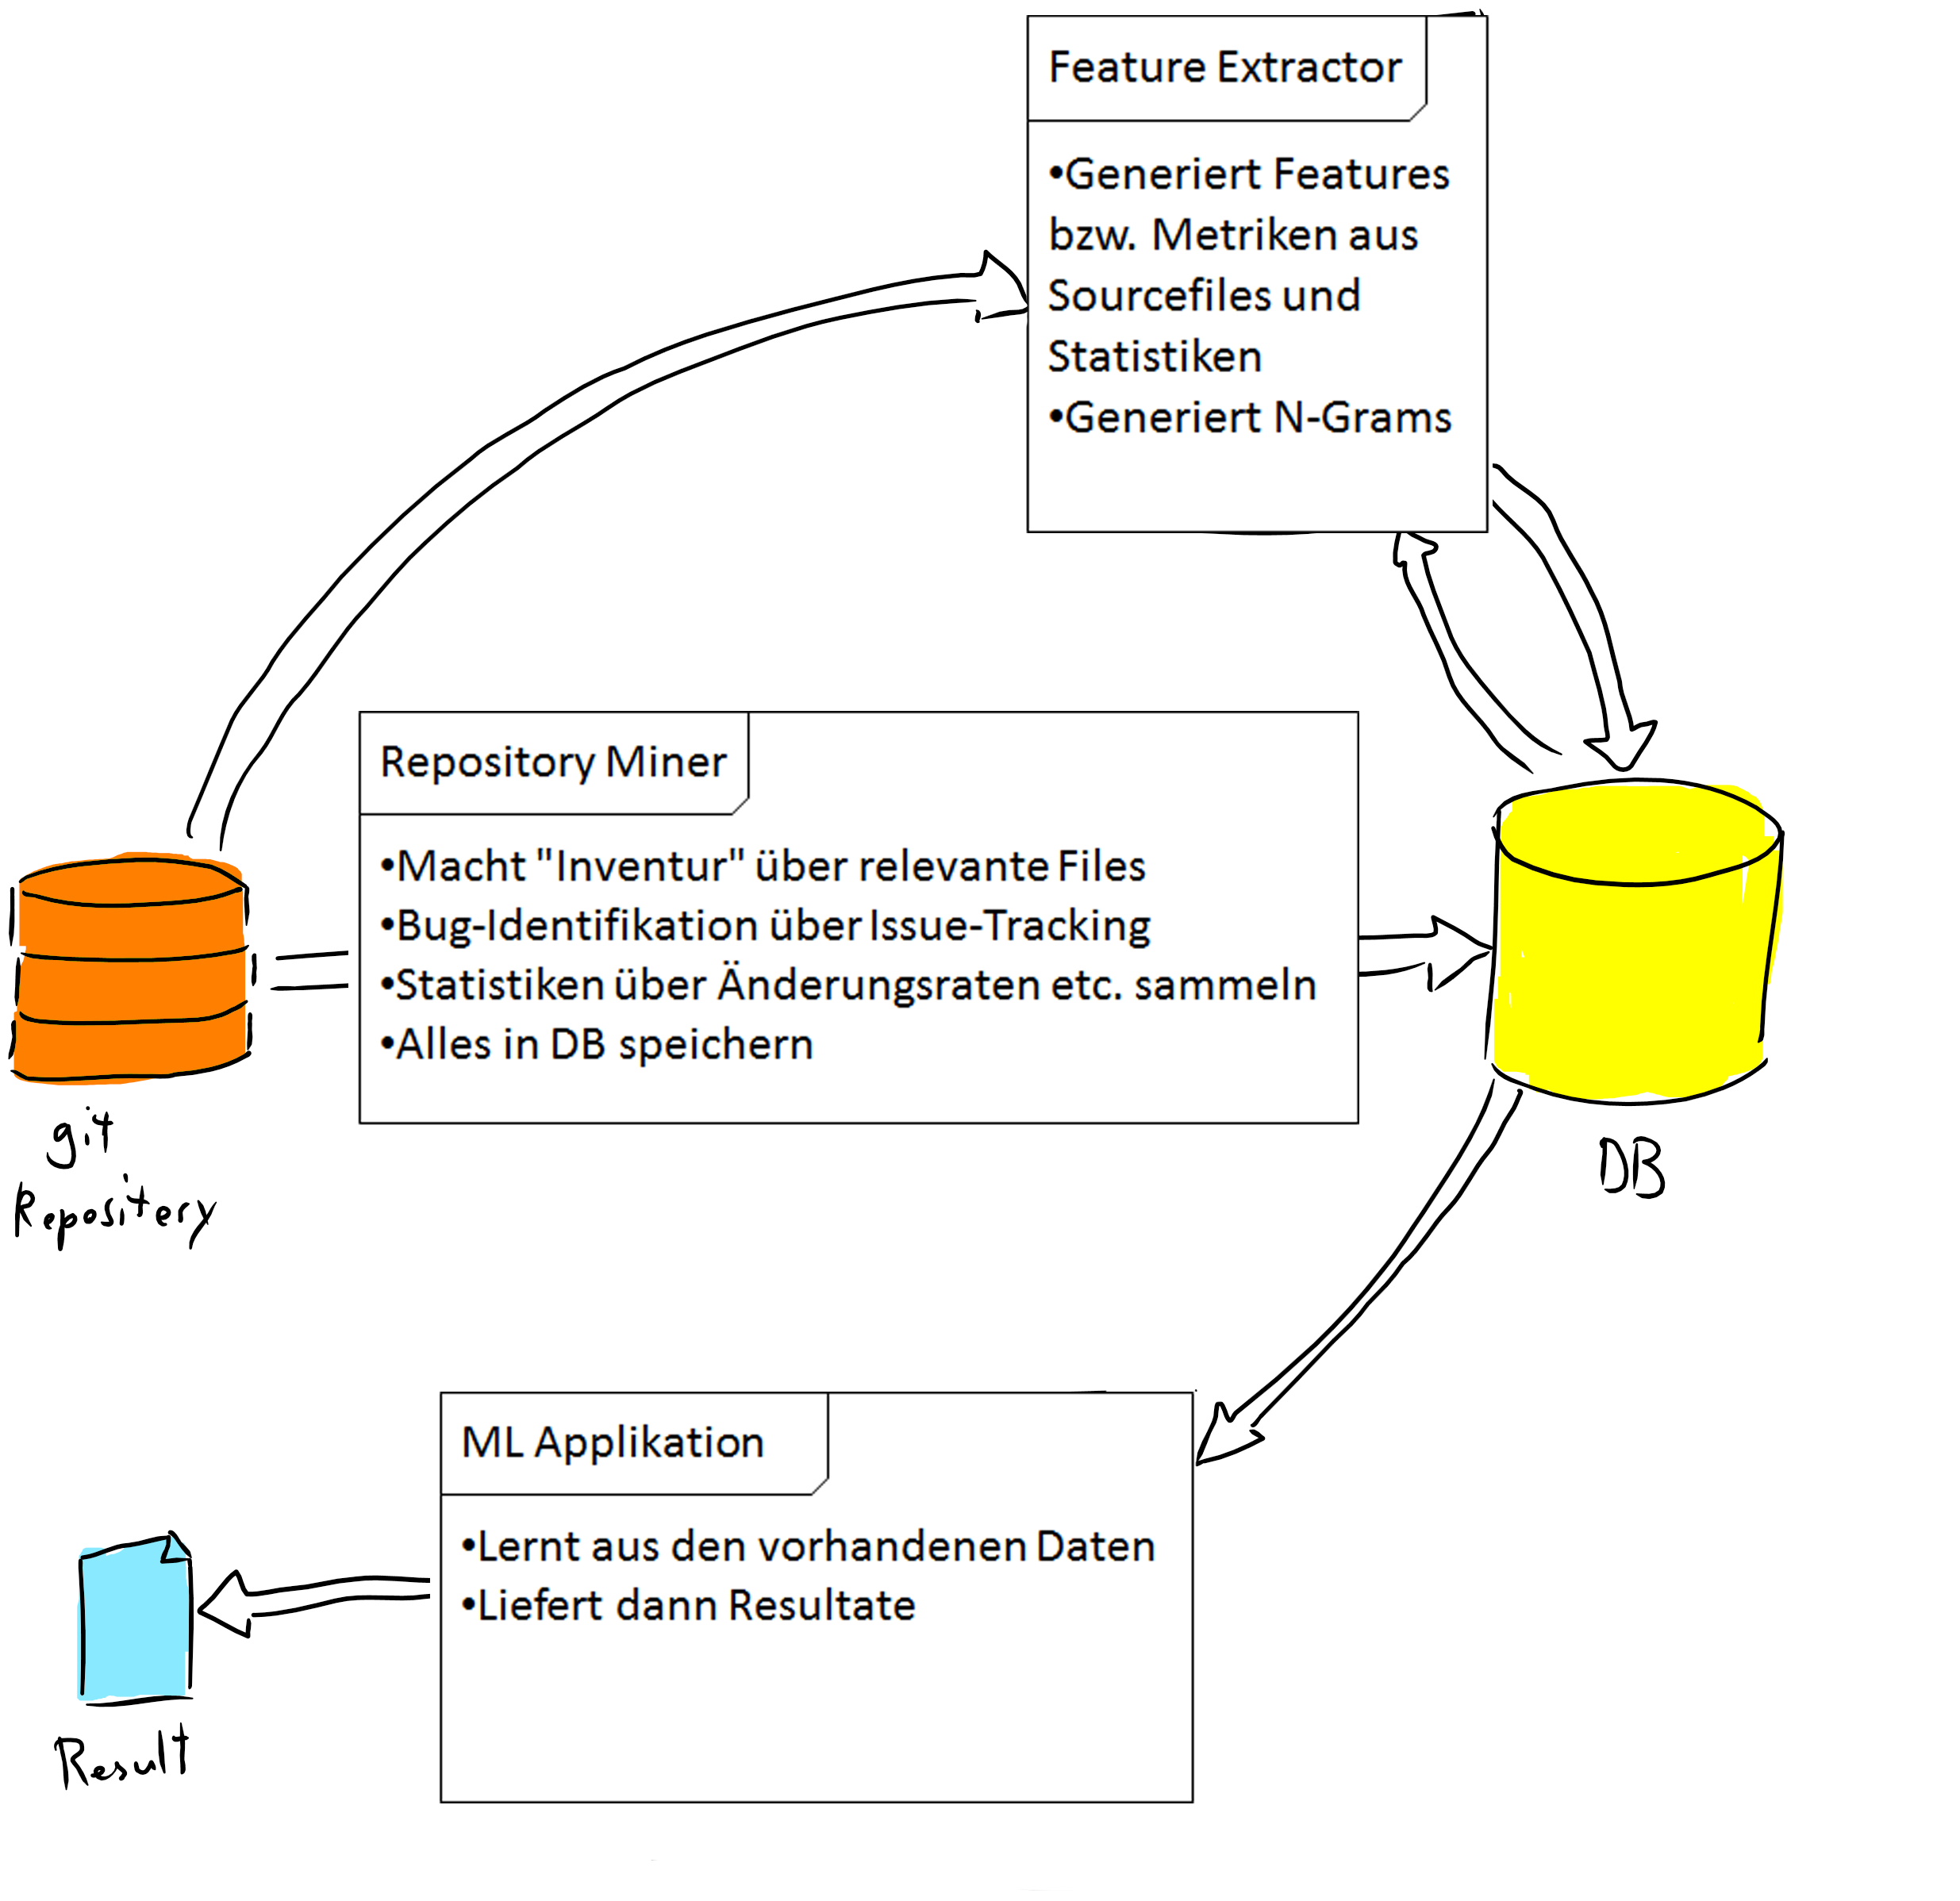
\includegraphics[width=1\textwidth]{resources/images/system_design.png}
	\caption{Grobübersicht des Systems}
	\label{systemdesign}
\end{figure}

In Abbildung \ref{systemdesign} wird die resultierende Systemarchitektur grob dargestellt.

% Was soll das System grob können (Details sind bei den einzelnen Komponenten beschrieben)
%% z. B. soll modular sein, damit die einzelnen komponenten später unabhängig voneinander weiterentwickelt/ausgetauscht werden können und das wir in sinnvollen arbeitsschritten und flexibel vorgehen können
%% Datenbank auch austauschbar, weil wir die Datenmenge noch nicht abschätzen können
%% systemunabhängige programmiersprachen (java, python), für zukünftige entwickler und für uns mit windows dev umgebung und linux server

% Wie ist das System aufgebaut -> Diagramm
%% Wieso die Unterteilung/Aufbau so wie angedacht
%%% z. B. Feature Extractor separat und nicht teil von ML-App, damit wir Features in der DB "cachen" können -> weniger speicherverbrauch / verlorene zeit
%%% Vllt. wieso RepositoryMiner und Issue Scanner nicht separat? -> vllt. weil datenmodell? ka
%%% später evtl. anders?
%% schnittstellen? --> DB

\subsubsection{Infrastruktur} \label{sec:infrastructure}

\ac{ML} mit einer grossen Anzahl an Features und Datensätzen ist sehr rechenintensiv. Die Berechnung auf einem der verwendeten Entwicklungscomputer durchzuführen war mangels genügend RAM und unzureichender CPU-Leistung nur begrenzt möglich. Uns war von Anfang an klar, dass die Projekte mit denen wir uns beschäftigen eine sehr grosse Anzahl Features generieren und deswegen auf einem dedizierten System ausgeführt werden müssen.

Die dafür genutzte Infrastruktur basiert auf einem \emph{Ubuntu Server 15.10 64 Bit}. Das System wird auf einer virtuellen \emph{VMWare vSphere 6.0} Infrastruktur ausgeführt und verfügt über 190 GB SSD Speicher (\emph{CRUCIAL SSD 480 GB M500}). Dem System stehen 8 Kerne einer \emph{Intel Xeon X5660 CPU} und 38 GB RAM zur Verfügung.
Der Datenbankserver und die in dieser Arbeit entwickelten Tools sind auf dem selben System installiert. Eine Separierung wäre natürlich möglich, hätte aber aufgrund von Ressourcenknappheit auf unserem System keinen grossen Vorteil gebracht.

\subsection{Repository Mining}\label{repositorymining}
Unser Repository Mining Tool erhielt das Akronym \emph{GtSooG} als Namen, was für \emph{Get the Stuff out of Git} steht. Die Hauptaufgabe von GtSooG besteht aus der Datenaufbereitung von \emph{Git}-Repositories und Issue-Tracking-Systemen. Die gesammelten Daten werden in einer SQL Datenbank gespeichert und dienen später als Grundlage für den Feature Extractor. 

Für diesen und das \ac{ML}-Tool ist performanter Zugriff auf die Datenbasis ein wichtiger Faktor. Ein direkter Zugriff auf Online-Ressourcen wäre für eine schnelle Verarbeitung undenkbar. 

Die Versionsverwaltung \emph{Git} hat den Vorteil, das ein lokaler Klon eines Repositories dessen komplette Revisionsgeschichte beinhaltet. Damit kann dieser unabhängig vom Server betrieben werden. Die Speicherverwaltung von \emph{Git} ist sehr effizient \cite{githubInternalsGitObjects}. Mit Hilfe von Deduplizierungsverfahren werden redundante Code-Objekte nur einmal gespeichert und untereinander verlinkt. Da wir nicht davon ausgehen, dies ansatzweise so effizient lösen zu können, verzichten wir auf die Speicherung des kompletten Codes in der Datenbank. Die Filter- und Suchmechanismen von \emph{Git} bieten allerdings nur eingeschränkte Möglichkeiten. Eine Suche resultiert meistens im Absuchen des ganzen Repositories und ist dementsprechend langsam.

Informationen über Issues werden separat in einem Issue-Tracking-System gespeichert. Diese Systeme werden meistens auf einem Server betrieben und können nicht lokal kopiert werden. Aufgrund dieser Tatsache ist das Abrufen von Issues eine schleppende Angelegenheit. Für das Issue-Tracking-System \emph{GitHub} kommt hinzu, dass der Zugriff auf die \emph{GitHub}-\acs{API} limitiert ist \cite{github:ratelimit}.

Die Aufgabe von GtSooG besteht darin, die oben erwähnten Limitierungen aufzuheben. Dies soll durch die strukturierte Speicherung der Metadaten von \emph{Git} und des Issue-Trackings in einer relationalen Datenbank bewerkstelligt werden. Damit ist nicht nur ein effizienter Zugriff gewährleistet, mit der mächtigen und weitverbeiteten \ac{SQL} lassen sich auch beliebig komplexe Abfragen erstellen.

\subsubsection{Anforderungen}
Die oben erwähnten Überlegungen führen zu folgenden Anforderungen:

\paragraph{Funktional:}
\begin{itemize}
	\item Zugriff auf lokal gespeicherte \emph{Git} Repositories
	\item Direkter Zugriff auf die Issue-Tracking-Systeme \emph{GitHub} und \emph{JIRA} über deren \acs{REST}-\acs{API}
	\item Datenspeicherung in einer \ac{SQL} Datenbank
	\item Speichern aller Commits, inkl. Autor und Commit-Datum
	\item Speichern aller Dateien, welche in einem Commit enthalten sind
	\item Speichern der verschiedenen Dateiversionen
	\item Speichern der geänderten Codezeilen pro Dateiversion
	\item Speichern aller Issues und die Zuordnung ob es sich um einen Bug handelt.
\end{itemize} 

\paragraph{Nichtfunktional:}
\begin{itemize}
	\item Modulare und erweiterbare Architektur
	\item Kommandozeilenbasiert
	\item Adäquates Errorhandling, so dass die Software bei einem nicht lesbaren Commit oder Issue die Arbeit fortsetzt (non-blocking)
	\item Die Ausführung von GtSooG soll jederzeit unterbrochen werden können, die gespeicherten Daten sollen trotzdem stets konsistent sein.
	\item Vermeiden redundanter Speicherung des Codes
\end{itemize} 

\paragraph{Abgrenzung:}
\begin{itemize}
	\item Es ist eine singlethreaded Architektur angedacht, Multithreading ist keine Anforderung
\end{itemize}

\subsubsection{Design}
Da sich die Schnittstellen von \emph{Git} und den verschiedenen Is\-sue-Track\-ing-Sys\-tem\-en fundamental unterscheiden ist GtSooG in folgende Komponenten unterteilt:
\begin{itemize}
	\item Der Repository Miner liest Daten direkt vom Dateisystem aus einem \emph{Git}-Repository aus und vertraut dabei auf die Funktionalität der \emph{gitpython} Library
	\item Der Issue Scanner liest Daten aus einem Issue-Tracking-System per \acs{REST}-\acs{API} aus
\end{itemize}
Die beiden Komponenten extrahieren folgende Informationen aus \emph{Git} und den Issue-Tracking-Systemen:
\begin{itemize}
	\item Name und Pfad des Repositories
	\item Alle Commits mit Mitteilung, Autor und Commit Datum
	\item Alle dem Commit angehängten Dateien mit Erstellungsdatum (entspricht Datum des Commits, mit dem sie erstellt wurden)
	\item Die verschiedenen Versionen der Dateien und die Anzahl von hinzugefügten und gelöschten Codezeilen
	\item Die hinzugefügten oder gelöschten Codezeilen pro Dateiversion
	\item Name und URL des Issue-Tracking-Systems
	\item Alle Issues mit Titel und der Information ob es sich dabei um einen Bug handelt
	\item Die Issues sollen den Commits zugeordnet werden können
\end{itemize}
\begin{figure}[!ht]
	\centering
	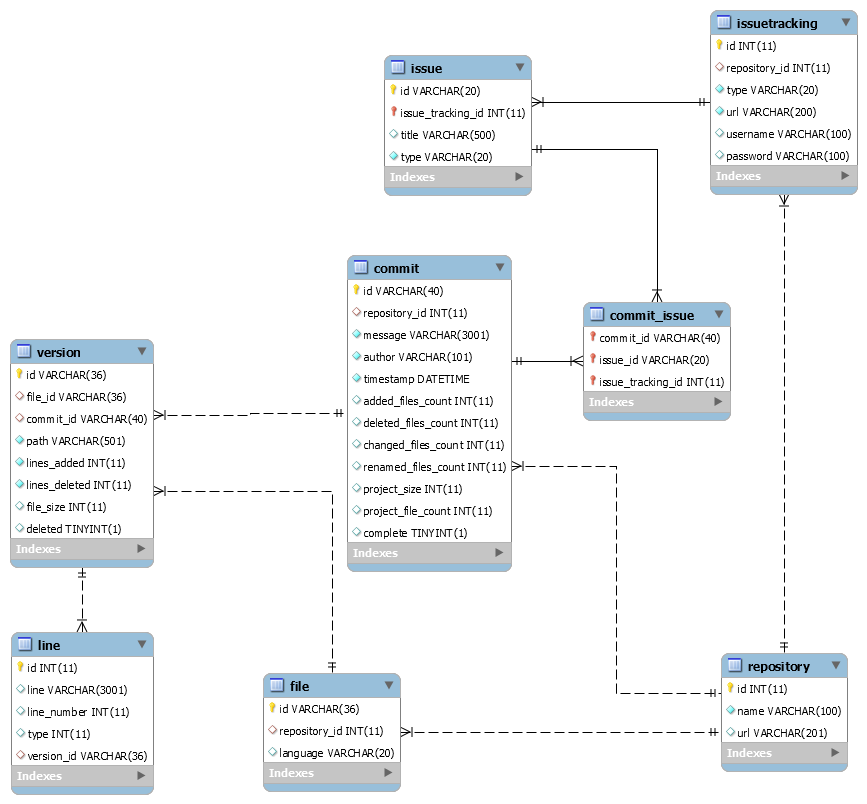
\includegraphics[width=1\textwidth]{resources/images/db_reverse_engineered_gtsoog.png}
	\caption{ERM GtSooG Datenbank}
	\label{fig:DBDesignGtSooG}
\end{figure}

Daraus resultierte das Datenbank Design in Abbildung \ref{fig:DBDesignGtSooG}. Die Felder \emph{files\_added} und \emph{files\_deleted} in der Tabelle \emph{version} sind redundant und könnten über eine SQL-Join-Query abgefragt werden. Da die Performance beim Feature Extractor eine grosse Rolle spielt, werden diese Informationen aber als zusätzliches Feld in der Datenbank gespeichert. Dasselbe gilt für die Felder\emph{ added\_files\_count}, \emph{deleted\_files\_count}, \emph{renamed\_files\_count}, \emph{changed\_files\_count} in der Tabelle \emph{commit}.

\subsubsection{Implementierung} \label{par:gtsoogtechnicalimplementation}
Der Repository Miner ist in Python geschrieben. Die Software macht Gebrauch von den Python-Bibliotheken \emph{request} \cite{pythonrequests}, \emph{GitPython} \cite{gitpython} und \emph{SQLAlchemy} \cite{sqlalchemy}.
\emph{GitPython} fungiert als Schnittstelle zum \emph{Git}-Repository. Ursprünglich sollte der Repository Miner mit Multithreading den Datamining-Prozess beschleunigen. Nach einigen Versuchen und Online-Recherche stellte sich dieser Prozess jedoch als sehr schwierig bis unmöglich heraus. Einerseits sind die einzelnen Commits voneinander abhängig was eine parallele Verarbeitung sehr komplex macht. Andererseits stellte sich heraus, dass das Unterfangen bereits vom Projekt \emph{gitpython/async} \cite{gitpythonasync} erfolglos versucht wurde. Es war somit nicht realistisch, im Rahmen dieses Projekts eine sinnvolle Lösung zu finden. Deshalb wurde der Repository Miner singlethreaded implementiert.
GtSooG liest die Commits sequentiell aus dem \emph{Git}-Repository. Pro Commit werden die Code-Änderungen verarbeitet. Eine Änderung erzeugt eine neue Version einer Datei. Die Zuordnung von Version zu Datei erfolgt über den Pfad der Datei. Pro Version analysiert GtSooG die geänderten Code Zeilen.
Der Issue Scanner ruft Issues vom Issue-Tracking-System via REST-Anfragen ab. Die Kadenz der Anfragen ist serverseitig von \emph{GitHub} und \emph{JIRA} begrenzt. Aufgrund dessen hätte ein Ansatz mit Multithreading keinen grossen Mehrwert gehabt. Die Abbildung \ref{fig:gtsoog_flowchart} visualisiert den Ablauf von GtSooG.
Den Datenbankzugriff übernimmt das \ac{ORM} Framework \emph{SQLAlchemy}. Das \ac{DBMS} im Hintergrund bleibt dadurch austauschbar. Anfangs wurde aufgrund der einfachen Handhabung mit \emph{SQLite} gearbeitet. Schnell wurde aber klar, dass dieses triviale \ac{DBMS} mit der anfallenden Datenmenge hoffnungslos überfordert ist. Das leistungsfähigere \emph{MySQL} löste \emph{SQLite} daher ab.

\begin{figure}[h]
	\centering
	\includegraphics[width=1\linewidth]{resources/images/gtsoog_flowchart}
	\caption[Programmablauf von GtSooG]{Der grobe Programmablauf von GtSooG}
	\label{fig:gtsoog_flowchart}
\end{figure}

\emph{GtSooG} soll die Daten stets in einem konsistenten Zustand hinterlassen. Da Commits voneinander abhängig sind, müssen sie entweder komplett (d. h. mit allen dazugehörigen Dateiversionen und geänderten Zeilen) oder gar nicht in der Datenbank gespeichert werden.
Um dies auch bei einem Systemabsturz zu gewährleisten, entschieden wir uns, das Datenbankfeld \emph{completed} in der Tabelle \emph{commit} einzuführen. Erst nach der erfolgreichen Verarbeitung eines Commits wird dieses Feld auf True gesetzt. Da beim Scannen von Issues kein Subprozess anfällt, waren dafür keine besonderen Massnahmen notwendig.

\subsubsection{Erkenntnisse} \label{sec:gtsoogfindings}

Die Arbeit mit der \emph{GitPython} Bibliothek stellte sich als schwierig heraus. Teile der von uns benötigten Funktionalität waren leider nicht vorhanden. Zum Beispiel existierte keine Funktion um die geänderten Zeilen pro Datei herauszufinden. \emph{GitPython} bot lediglich den String-Output des \emph{diff} Programms an. Dieser musste manuell geparst werden. Die Entwicklung und das Testing stellte sich als schwierig heraus. Die immense Datenmengen von unterschiedlichen Repositories erzeugten immer wieder Spezialfälle in den \emph{diff}-Strings, was zu Fehlern in GtSooG führte. Da es für Python keine anderen, nennenswerten \emph{Git}-Bibliotheken gab, hätten wir uns bei der Wahl der Programmiersprache im Nachhinein wohl besser für Java entschieden. Damit ist mit \emph{Eclipse JGit} \cite{jgit} eine etablierte \emph{Git}-Bibliothek verfügbar.

\subsection{Feature Extractor} \label{sec:featureextractor}
Die Aufgabe des Feature Extractors besteht darin, die für das \ac{ML} benötigten Features (siehe Kapitel \ref{sec:features}), aus den gesammelten Daten zu generieren. Die Datenbasis besteht aus der von GtsooG erstellten Datenbank und dem entsprechenden \emph{Git}-Repository im Dateisystem. Um die von der Gesamtarchitektur angestrebte Modularität zu gewährleisten, soll der Feature Extractor die generierten Features anschliessend in der \ac{DB} speichern. Dafür entschieden wir uns trotz anfänglicher Bedenken bezüglich der grossen Datenmenge. Der Entscheidung liegen folgende Überlegungen zu Grunde:
\begin{itemize}
	\item Die Verwendung der identischen Technologie wie GtSooG vereinfacht die Architektur.
	\item Es kann ein schneller Zugriff durch die strukturierte Speicherung der Daten in der Datenbank sichergestellt werden.
	\item Durch strikte Verwendung eines \acp{ORM} ist das \ac{DBMS} austauschbar und somit nicht an Speicherlimits von Herstellern gebunden
	\item Das \ac{DBMS} kann einfach von den restlichen Komponenten entkoppelt werden
\end{itemize}

 \subsubsection{Anforderungen}
Der Feature Extractor soll folgende Anforderungen erfüllen:

\paragraph{Funktional:}
\begin{itemize}
	\item Zugriff auf die von GtSooG in der Datenbank gespeicherte Datenbasis
	\item Zugriff auf die zugehörigen \emph{Git}-Repositories
	\item Generieren eines Java \ac{AST} aus Java Code
	\item Speichern der generierten Features in der SQL-Datenbank
	\item Korrekte Berechnung der im Kapitel \ref{sec:features} beschrieben Features
\end{itemize} 

\paragraph{Nichtfunktional:}
\begin{itemize}
	\item Modulare und erweiterbare Architektur
	\item Kommandozeilenbasiert
	\item Verarbeitung mit Multithreading
	\item Einzelne Features sollen testbar sein
	\item Soll mit wenig Aufwand um zusätzliche Features erweitert werden können
\end{itemize} 

\subsubsection{Design}
Der Feature Extractor wurde in drei Komponenten unterteilt:
\begin{itemize}
	\item Die Feature Berechnung 
	\item Die Datenbankanbindung per \ac{ORM}
	\item Die Datenanbindung für die \emph{Git}-Repository
\end{itemize}

Die extrahierten Features werden in der von GtSooG angelegten Datenbank gespeichert. Um dies zu ermöglichen, musste das Datenmodell um die Tabellen \emph{feature\_value} und \emph{ngram\_vector} erweitert werden. In der Abbildung \ref{fig:FeatureExtractor} sind die neuen Tabellen der Datenbank farblich gekennzeichnet.

\begin{figure}[!ht]\label{featureextractordbdesign}
	\centering
	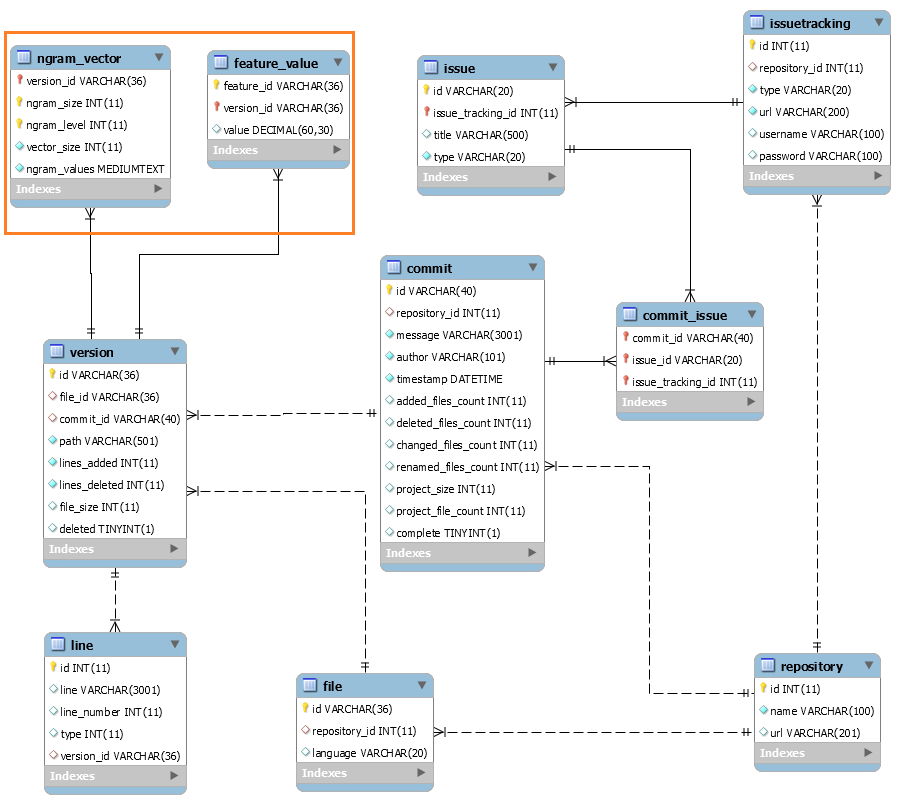
\includegraphics[width=1\textwidth]{resources/images/db_reverse_engineered_feature_extractor.png}
	\caption{ERM der GtSooG Datenbank mit Feature Extractor Erweiterungen}
	\label{fig:FeatureExtractor}
\end{figure}

Alle Features ausser N-Grams werden in der Tabelle \emph{feature\_value} gespeichert. Sie beinhaltet die Kennzeichnung des Features (\emph{feature\_id}), eine Referenz zur dazugehörigen Version (\emph{version\_id}) und den berechneten Wert (\emph{value}).
In der \emph{feature\_value}-Tabelle werden pro Version alle Features gespeichert. Mit einer grossen Anzahl Dateiversionen wächst die Grösse der Tabelle rapide an. Dieses Design bietet jedoch die Möglichkeit, einfach nach einzelnen Features filtern zu können.

Da wir bei den N-Grams verschiedene Längen und verschiedene Levels haben (siehe Kapitel \ref{par:ngrams}) und auch danach filtern wollen, ist eine separate Tabelle (\emph{ngram\_vector}) notwendig. Der berechnete Feature-Wert der N-Grams (entspricht der Anzahl Vorkommnisse) wird als Komma-separierter String im Feld \emph{ngram\_values} hinterlegt. Auf diese Weise kommen auf jede Version nur wenige N-Gram-Datensätze, was die Tabelle klein hält. Trotzdem ist es noch möglich, auf bestimmte N-Gram-Kategorien zu selektieren. Die Selektion einzelner N-Grams ist keine Anforderung.

\subsubsection{Implementierung}
Der Feature Extractor ist in Java implementiert. Diese Entscheidung ist auf den Umstand zurückzuführen, dass für einige Features das Parsen und Analysieren von Java-Code nötig ist. \emph{Eclipse JDT AST} \cite{eclipsejdtast} ist eine einfach zu handhabende Java-Bibliothek, welche diese Aufgabe erfüllen kann. Sie bietet die Funktionalität, Java-Source-Code als \acf{AST} darzustellen. Ausserdem befreit \emph{Eclipse JDT AST} den Source Code automatisch von Namen und ermöglicht somit einen Vergleich mit anderen Source-Code-Dateien. Unter den Java-Syntaxparsern stellte sich \emph{Eclipse JDT AST} gegenüber anderen Implementationen wie \emph{javaparser} \cite{javaparser} als die mächtigste und weitverbreitetste Bibliothek heraus.

\paragraph{Ablauf und Erweiterbarkeit}
Der Feature Extractor liest zuerst die Versionen und Commits aus der Datenbank in den Arbeitsspeicher. Dann iteriert er durch die verschiedenen Versionen. Pro Version werden die konfigurierten Features berechnet. Um dabei eine bessere Leistung zu erzielen, werden ähnliche Features in Featuregruppen zusammengefasst. Zum Beispiel werden die Lines-of-Code-Features PLOC, SLOC, BLOC und CLOC in der Featuregruppe \emph{LinesOfCodeFeatureGroup} zusammengefasst. 

\begin{figure}[h]
	\centering
	\includegraphics[width=1\linewidth]{resources/images/feature_extractor_packages}
	\caption[Packages vom Feature Extractor]{Die Package-Struktur des Feature Extractors (grob vereinfacht)}
	\label{fig:feature_extractor_packages}
\end{figure}

Das Hinzufügen von Features ist sehr einfach: Es muss eine neue Klasse erstellt werden, die das \emph{IFeatureGroup} Interface und deren Methode \emph{extract} implementieren. In dieser Methode ist die Berechnung des oder der Features implementiert. Zusätzlich muss sich die Klasse im Package \emph{features} befinden (siehe Abbildung \ref{fig:feature_extractor_packages}). Der Feature Extractor iteriert automatisch mittels Reflection durch alle Klassen in diesem Package und ruft deren Methode \emph{extract} auf. Als Rückgabewert erhält er eine HashMap. Diese Map hat als Key die Feature-Bezeichnung und als Value den dazugehörigen Wert. Die Implementation der \emph{extract}-Methode erhält folgende Argumente:
\begin{itemize}
	\item Den Java Source Code
	\item Den AST-Code
	\item Die aktuelle Version
	\item Eine Liste aller Commits
\end{itemize}
Der Java-Source-Code wird direkt aus einem \emph{Git}-Repository ausgelesen. Dies übernimmt die \emph{Git}-Komponente mit Hilfe der \emph{JGit}-Bibliothek. Die Datenbankanbindung wurde mit dem weitverbreiteten \ac{ORM} \emph{HibernateORM} realisiert.

\paragraph{Datenzugriff}

Der Feature Extractor generiert eine grosse Anzahl von Daten. Diese Aufgabe ist weitaus anspruchsvoller als diejenige von GtSooG. Das Repository von \emph{Elasticsearch} mit 10 Jahren erfasster Entwicklung umfasst 21'740 Commits und über 100'000 Dateiversionen. Daraus generiert der Feature Extractor 10 GB herkömmliche Features und 120 GB N-Grams. Bei der ersten Version des Feature Extractors stellte sich das Speichern der Daten in der \ac{DB} als Flaschenhals heraus. Der \ac{DB}-Server verzeichnete trotz Verwendung von SSDs eine Harddisk-Auslastung von 100\% über den gesamten Durchlauf. Die effektive Schreibrate betrug aufgrund der Datenbank und der Implementierung lediglich ca. 0.5 MByte/s.

Folgende Optimierungsmassnahmen sollten den Datenbankzugriff beschleunigen:
\begin{itemize}
	\item Es werden alle benötigten Daten (Versionen, Commits, Issues) beim Programmstart eingelesen um die Anzahl Lesezugriffe auf die Datenbank zu reduzieren.
	\item Bulk-Writing: Anstatt alle Features für jede Version einzeln zu schreiben, werden Schreiboperationen zusammenfassen.
\end{itemize}
Die Massnahmen zeigten Wirkung und die durchschnittliche Schreibrate stieg auf ca. 5 MByte/s. Weiteres Optimierungspotential wurde beim \ac{DBMS}, in diesem Fall \emph{MySQL} festgestellt. Normalerweise hat die Beständigkeit und Konsistenz der Daten in einer Datenbank höchste Priorität. Für die ML-Pipeline ist die Geschwindigkeit allerdings wichtiger. Deswegen haben wir uns entschieden, bei einer Schreiboperation nicht auf die definitive Schreibbestätigung (fsync) zu warten und die Daten asynchron zu schreiben. Daraus resultierten folgende Einstellungen für den SQL Server:

\begin{minipage}{\linewidth}
\begin{lstlisting}[frame=single,caption={MySQL Konfiguration}]
innodb_log_buffer_size=2G
innodb_flush_log_at_trx_commit=0
innodb_flush_method=nosync
skip-innodb_doublewrite
\end{lstlisting}
\end{minipage}

Es ist uns bewusst, dass bei einem Rechnerabsturz die Wahrscheinlichkeit eines Datenverlusts dadurch steigt. Diese Einstellungen führten aber zu einer immens höheren Schreibrate von ungefähr 25 MByte/s.

\subsubsection{Erkenntnisse}

Der Umgang mit dem Eclipse AST stellte sich teilweise als gewöhnungsbedürftig heraus. Features wie N-Grams und CodeComplexity sind besonders stark auf die Funktionalitäten von AST angewiesen. Da die verschiedenen Node-Typen (Klassen, Methoden, Variablen) teilweise für ähnliche Eigenschaften (zum Beispiel um alle Childnodes abzurufen) verschiedene Methoden verwenden, ist eine aufwendige Node Unterscheidung im Code notwendig. Dies führte zu viel und kompliziertem Code. Beim Vergleich mit anderen Projekten schien es dafür allerdings keine bessere Lösung zu geben. 

\subsection{Features} \label{sec:features}
Features sind die messbaren Eigenschaften einer Beobachtung, auf deren Basis ein \ac{ML}-Algorithmus trainiert wird, um dann anschliessend Resultate vorherzusagen. Ein Beispiel soll die Wichtigkeit von gut ausgewählten Features erläutern. 

Eine Immobilienfirma versucht, Grundstückspreise anhand der Grund\-stücks\-flä\-che vorherzusagen. Dies ist eine typische \ac{ML}-Aufgabe und kann in diesem Fall mit Hilfe von Linearer Regression gelöst werden. Das dabei eingesetzte Feature ist die Grundstücksfläche. Die Abbildung \ref{fig:housing_prices} zeigt einen Lerndatensatz mit der Grundstücksfläche als Feature auf der X-Achse und die dafür bekannten Grundstückspreise auf der Y-Achse.
Der Zusammenhang ist trivial und die resultierende Regressionsgerade kann eine nahezu perfekte Vorhersage machen.

\begin{figure}[!ht]
	\centering
	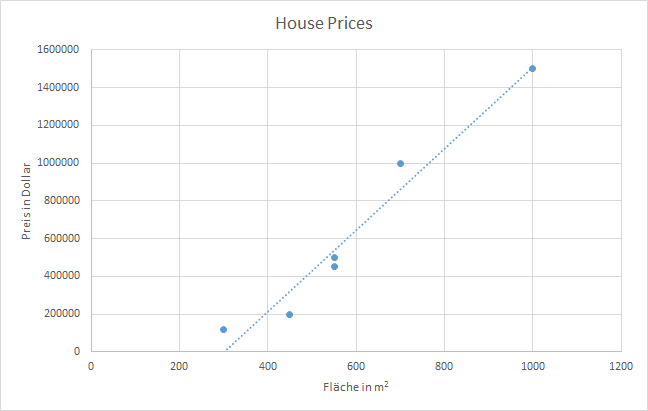
\includegraphics[width=0.75\textwidth]{resources/images/housing_prices_with_trendline.png}
	\caption{Vorhersage Grundstückspreise}
	\label{fig:housing_prices}
\end{figure}

Das Beispiel zeigt, dass die richtige Auswahl der Features grossen Einfluss auf das Resultat der \ac{ML}-Applikation hat. Anzumerken ist, dass in realen Szenarien die Anzahl Features meist ein Vielfaches beträgt. Auch besteht in der Regel kein trivialer linearer Zusammenhang.

Eine der Herausforderungen dieser Arbeit war es, aus Java-Source-Code-Dateien sinnvolle Features zu bestimmen, welche für die Problemstellung, also der Fehlervorhersage, nützlich waren. Feature Design (auch Feature Engineering) ist oft ein schwieriger und zeitaufwändiger Prozess. Deshalb wurde sich hier zu einem grossen Teil auf bestehende Arbeiten gestützt.

Das folgende Kapitel soll eine Übersicht und detaillierte Beschreibung über die implementierten Features geben und schlägt auch einige Features vor, mit denen das Ergebnis in Zukunft noch weiter verbessert werden könnte.

\subsubsection{Lines-of-Code-Features}
Die Lines-of-Code-Features werden pro Dateiversion über den Source Code berechnet, unabhängig davon wie viele Klassen, Enums und Interfaces sich in einer Java-Source-Code-Datei befinden.
\begin{table}[H]
	\begin{tabular}{l|p{3cm}|p{5.75cm}}
		\textbf{Abkürzung} & \textbf{Name} & \textbf{Beschreibung}\\
		\hline
		PLOC 	& Physical lines of code& Zeilenanzahl einer Dateiversion im Total\\
		SLOC 	& Total lines of code 	& Zeilen, die Java Code enthalten\\
		CLOC 	& Comment lines of code & Anzahl Zeilen, die einen Kommentar enthalten\\
		BLOC 	& Blank lines of code 	& Leere Zeilen\\
		MINLINE & minimal line length 	& Minimale Zeilenlänge\\
		MAXLINE & maximal line length 	& Maximale Zeilenlänge\\
		MEDLINE & median line length 	& Median der Zeilenlängen\\
	\end{tabular}
	\caption{Lines-of-Code-Features}
	\label{tab:linesofcodefeatures}
\end{table}

Da wir erwarteten, dass die Länge der einzelnen Codezeilen wahrscheinlich von Zeile zu Zeile sehr unterschiedlich sein wird, machte es keinen Sinn, diese einzeln zu erfassen. Stattdessen wurde der Mittelwert der Zeilenlänge verwendet. Als Mittelwert wurde bewusst der Median gewählt, da er robust gegenüber Ausreissern ist. Die Extreme wurden durch die maximale und minimale Zeilenlänge aufgezeichnet.

Die ausgewählten Features stützen sich auf mehrere Quellen. Sowohl Liljeson und Mohlin \cite{Liljeson831487} über statische Code-Analyse und \ac{ML} als auch Moriggl et al. \cite{Moriggl831473} und Nagappan et al. \cite{Nagappan:2005:URC:1062455.1062514} verwenden in ihren Arbeiten Lines-of-Code-Features. 

Ein grosser Effekt wurde von den Lines-of-Code-Features nicht erwartet. Allerdings waren sie dank geringem Implementationsaufwand schnell einsatzfähig und boten eine gute Grundlage für die ersten Gehversuche mit \ac{ML}. Hinzu kam, dass diese Features in diversen Arbeiten erwähnt wurden.

\subsubsection{Objektorientierte Features} \label{sec:objectorientedfeatures}
Objektorientierte Metriken wurden bereits öfters zur Fehlervorhersage verwendet. So zum Beispiel von Gyimothy et al. \cite{Gyimothy:2005:EVO:1100866.1100985} und Siket et al. \cite{Siket08} auf verschiedenen Open-Source-Projekten. Es sind zudem die einzigen Features, welche die Eigenschaften von objektorientiertem Programmieren erfassen sollen. Deshalb war anzunehmen, dass diese gerade bei Java einen signifikanten Einfluss auf das Resultat haben könnten.

Wie die Lines-of-Code-Features berechnet der Feature Extractor die objektorientierten Features pro Java-Source-Code-Datei. Befinden sich mehrere Klassen, Enums oder Interfaces in einer Java-Source-Code-Datei werden die Features pro Klasse erfasst. Falls pro Datei mehrere Klassen vorhanden sind, werden die Feature-Werte pro Dateiversion zusammengezählt.

\begin{table}[H]
	\begin{tabular}{l|p{3cm}|p{5.75cm}}
		\textbf{Abkürzung} & \textbf{Name} & \textbf{Beschreibung}\\
		\hline
		WMC & Weighted methods per class & Anzahl Methoden pro Klasse (inkl. Konstruktoren)\\
		CBO & Coupling between objects & Die Anzahl der nicht zur Klasse gehörenden Methodenaufrufe\\
		RFC & Response for class & WMC und CBO zusammengezählt.\\
		LCOM & Lack of cohesion in methods & Anzahl Klassenmethoden die nicht auf eine Klassenvariable zugreifen\\
		NPM & Number of public methods & Anzahl Klassenmethoden mit dem Modifier public\\
		NPV & Number of public variables & Anzahl Klassenvariablen mit dem Modifier public\\
	\end{tabular}
	\caption{Objektorientierte Features}
	\label{tab:objectorientedfeatures}
\end{table}

Die objektorientierten Features wurden weitgehend aus der Arbeit von Liljeson und Mohlin \cite{Liljeson831487} übernommen. Die objektorientierten Features Depth of Inheritance Tree (DIT), Number of Children (NOC) und Afferent coulings (AC) benötigen zur Berechnung den Source Code des gesamten Projekts. Da der Feature Extractor Dateiversionen isoliert behandelt, ist die Betrachtung des ganzen Source Codes sehr aufwendig. Aufgrund dessen und weil wir den Fokus auf Textanalyse-Features gelegt haben, wurden diese Features nicht implementiert. Eine spätere Erweiterung des Feature Extractors ist möglich.

\subsubsection{Code-Complexity-Features} \label{sec:complexityfeatures}
Die Literaturrecherche hat gezeigt, dass bei statischer Code-Analyse Komplexitätsmetriken schon seit langem miteinbezogen werden. Es erschien uns deshalb als sinnvoll, eine Auswahl der bekanntesten Code-Komplexitätsmetriken als Features zu implementieren. Wir erhofften uns im besten Fall eine Kausalität zwischen Software-Komplexität und Softwarefehlern. Die Entscheidung fiel auf Metriken nach Halstead \cite{Halstead:1977:ESS:540137} und McCabe \cite{mccabe1976}. Begründen lässt sich die Auswahl aufgrund der Bekanntheit und Etabliertheit der beiden Metriken.

Das Herzstück der Halstead-Metrik sind folgende aus dem Source Code extrahierten Werte:

\begin{table}[H]
	\begin{tabular}{l|l}
		\textbf{Abkürzung} & \textbf{Beschreibung}\\
		\hline
		n1 & Anzahl eindeutiger Operatoren\\
		n2 & Anzahl eindeutiger Operanden\\
		N1 & Vorkommnisse der Operatoren im Code\\
		N2 & Vorkommnisse der Operanden im Code\\
	\end{tabular}
	\caption{Healstead-Operanden und -Operatoren}
	\label{tab:halsteadoperands}
\end{table}

Daraus werden anschliessend diverse Kennwerte wie zum Beispiel die Anzahl zu erwartende Bugs (nach Halstead) oder der Programmieraufwand berechnet. Da die Halstead-Metrik lange vor Java definiert und entwickelt worden ist, war die grösste Herausforderung das Einordnen der Java-Objekte in die beiden Klassen Operatoren und Operanden. Die Implementierung dieser Arbeit lehnt sich an die Arbeit von Dinari et al. \cite{halstead:dinari} an.

Die McCabe Metrik ist weiter verbreitet. Es existieren in Java geschriebene Eclipse-Plugins zur automatischen Berechnung. Unsere Implementation lehnt sich stark an das Eclipse-Plugin \emph{metrics2} \cite{metrics2} an.

Aus den beiden Metriken entstehen folgende Features:

\begin{longtable}{l|p{3cm}|p{5.75cm}}
		\textbf{Abkürzung} & \textbf{Name} & \textbf{Beschreibung}\\
		\hline
		n1 & n1 & Anzahl eindeutiger Operatoren\\
		n2 & n2 & Anzahl eindeutiger Operanden\\
		N1 & N1 & Vorkommnisse der Operatoren im Code\\
		N2 & N2 & Vorkommnisse der Operanden im Code\\
		n & Vocabulary length & n1 + n2 \\
		N & Program length & N1 + N2\newline\\
		\(\hat{N}\) & Calculated program length & \(n1*\log_2{n1} + n2*\log_2{n2}\)\\
		V & Volume\newline & \(N*\log_2{n}\)\\
		E & Effort\newline & \(\frac{n1}{2} * \frac{N2}{n2}\)\\
		T & Time required to program & \(\frac{effort}{18}\)\\
		B & number of bugs & \(\frac{effort^\frac{2}{3}}{3000}\)\\
		mccabeTotal & McCabe-Total\newline & McCabe Metrik für die ganze Version\\
		mccabeMethod & McCabe per Method\newline & McCabe Metrik pro Methode \(\frac{mccabeTotal}{MethodCount}\)\\
		mccabeClass & McCabe per Class & McCabe Metrik pro Klasse \(\frac{mccabeTotal}{ClassCount}\) \newline\\
		mccabeClassMethod & McCabe per Method and Class & McCabe Metrik pro Klasse und Methoden  \(\frac{mccabeTotal}{ClassCount*MethodCount}\)\\
	\caption{Code-Complexity-Features}
	\label{tab:codecomplexityfeatures}
\end{longtable}

\subsubsection{Anzahl-und-Typen-Features}
Die Auswirkung von Anzahl-und-Typen-Features ist schwer vorherzusagen. Vielleicht können triviale Java Klassen, welche bloss ein Datenmodell abbilden, von fehleranfälligen Klassen mit vielen komplexen Methoden unterschieden werden. Da diese Features einfach zu implementieren sind, wurden sie integriert.

Die Anzahl-und-Typen-Features konzentrieren sich auf die Vorkommnisse von High-Level-Elementen in einer Java-Version. Zu den High-Level-Elementen zählen:

\begin{itemize}
	\item Imports
	\item Klassen
	\item Interfaces
	\item Enums
	\item Methoden
	\item Klassenvariablen
	\item Klassenkonstanten
	\item lokale Variablen
\end{itemize}

Konstanten werden durch in Java über final static Modifiers identifiziert.
Für Klassen, Interfaces, Enums, Methoden, Klassenvariablen und Klassenkonstanten wird die Anzahl Vorkommnisse ausserdem pro Modifier (public, private und protected) gezählt.

\subsubsection{Temporale Features} \label{sec:temporalfeatures}
Die temporalen Features machen sich dem Namen entsprechend zeitabhängige Informationen der Versionsverwaltung zunutze. Die einzelnen Features sollen vom Zeitpunkt der aktuellen Dateiversion über eine Zeitspanne berechnet werden.

Die von GtSooG gesammelten Metadaten über das \emph{Elasticsearch} Projekt werden im Kapitel \ref{sec:filesamplestatistics} analysiert und mit Hilfe von Statistiken grafisch dargestellt. Die Auswertung offenbarte interessante Details über den Zusammenhang von Enhancements und Bugs. Werden viele Erweiterungen erzeugt, folgen mit einer zeitlichen Verzögerung eine erhöhte Anzahl von Bugs. Diese Informationen erschienen uns für die Vorhersage von Bugs als sehr wichtig und wurden deswegen in Form temporaler Features aufgenommen. Da viele Änderungen am Source Code auch die Bug-Wahrscheinlichkeit erhöhen, sind als weitere Features die Anzahl geänderter Dateien, sowie die Anzahl hinzugefügter und gelöschter Zeilen als Features erfasst.

Wir entschieden uns diese Werte über mehrere Zeitspannen zu speichern. Die Abstände der Zeitspannen wurden bewusst nicht linear gewählt, sodass mit nur sieben Zeitspannen einen möglichst grosser Zeitraum von 2 Jahren abgedeckt werden kann.
\begin{itemize}
	\item 1 Tag
	\item 1 Woche
	\item 1 Monat
	\item 3 Monate
	\item 6 Monate
	\item 1 Jahr
	\item 2 Jahre
\end{itemize}
Die folgenden Features werden pro Zeitspanne berechnet:

\begin{table}[H]
	\begin{tabular}{l|p{3cm}|p{5.75cm}}
		\textbf{Abkürzung} & \textbf{Name} & \textbf{Beschreibung}\\
		\hline
		NOAL & Number of added lines & Anzahl hinzugefügter Zeilen über einen Zeitraum\\
		NODL & Number of deleted lines & Anzahl gelöschter Zeilen über einen Zeitraum\\
		NOA & Number of authors & Anzahl verschiedener Autoren über einen Zeitraum\\
		NOB & Number of bugs & Anzahl Bugfixes über einen Zeitraum\\
		NOE & Number of enhancements & Anzahl Enhancements über einen Zeitraum\\
	\end{tabular}
	\caption{Temporale Features}
	\label{tab:temporalfeatures1}
\end{table}

Aus der Kombination der Zeitspannen und den Features ergeben sich insgesamt 30 Features. Das Beispiel ``number of added lines per month'' wird in der Datenbank als NOAL30D gespeichert. Der Feature Extractor sucht vom Zeitpunkt der Dateiversion 30 Tage in die Vergangenheit nach Commits, welche eine ältere Version derselben Datei enthalten. Für jeden Commit werden die Anzahl hinzugefügter Zeilen aufsummiert.

Die Anzahl geänderter Dateien pro Commit werden für alle oben auf\-ge\-führ\-ten Zeitspannen berechnet. In einer der oben aufgelisteten Zeitspannen können mehrere Commits sein. Da die Anzahl der Commits in der Zeitspanne von Version zu Version unterschiedlich ist, erfassen wir von den folgenden Veränderungstypen den Median, den Mittelwert, das Maximum und das Minimum.
\begin{table}[H]
	\begin{tabular}{l|p{3cm}|p{5.75cm}}
		\textbf{Abkürzung} & \textbf{Name} & \textbf{Beschreibung}\\
		\hline
		NOAF & Number of added files & Anzahl hinzugefügter Dateien über einen Zeitraum\\
		NODF & Number of deleted files & Anzahl gelöschter Dateien über einen Zeitraum\\
		NOCF & Number of changed files & Anzahl geänderter Dateien über einen Zeitraum\\
		NORF & Number of renamed files & Anzahl umbenannter Dateien über einen Zeitraum\\
	\end{tabular}
	\caption{Temporale Features - geänderte Dateien}
	\label{tab:temporalfeatures2}
\end{table}

Ein weiteres Feature, DBLC (Days between last commit), berechnet die Anzahl Tage zwischen dem Commit mit der aktuellen Version und dem vorherigem Commit, welcher die Dateiversion enthält. Damit soll die Zeitspanne bis zur letzten Änderung der Datei erfasst werden.

\subsubsection{Textanalyse-Features}
In der Text- und Sprachanalyse werden verschiedene Analyseverfahren zur Detektion von Bedeutungsstrukturen eingesetzt. In Programmiersprachen ist die Bedeutung von Wör\-tern normalerweise eindeutig. Durch Kombination der Wör\-ter entsteht die Programmlogik, welche man im entferntesten Sinne mit der Semantik einer natürlichen Sprache vergleichen kann. Daraus entstand die Idee, Textanalyse-Features auf eine Programmiersprache anzuwenden.
Eine Programmiersprache weist grundsätzlich eine einfachere Grammatik auf. Zum Beispiel entfallen Konjugationen von Wörtern. Dadurch gibt es weniger Interpretationsspielraum. Auch erhoffen wir uns daraus bei den N-Gram Features eine geringe Anzahl von Daten zu erhalten.

Einen guten Überblick über verschiedene Textanalyse-Features liefert Mohammad et al. mit ihrer Arbeit über Twitter-Sentiment-Analyse \cite{DBLP:journals/corr/MohammadKZ13}. Aus dieser Arbeit erschienen uns N-Grams und die Länge von Namen als vielversprechend. Die N-Grams könnten verschiedene Anordnungen von Java-Code-Wörtern, welche einem Bug zugeordnet sind, identifizieren und diese in einer zukünftigen fehlerbehafteten Versionen wiedererkennen. Die Länge von Namen soll die Einhaltung von Code Style (Naming-Konventionen) prüfen. Vielleicht ist ein Nichteinhalten ein Indiz auf einen Softwarefehler.

\begin{longtable}{l|p{3cm}|p{5.75cm}}
		\textbf{Abkürzung} & \textbf{Name} & \textbf{Beschreibung}\\
		\hline
		MINVAR & Minimal variable name length & Der kürzeste Variablenname der Klasse und deren Methoden\\
		MAXVAR & Maximal variable name length & Der längste Variablenname der Klasse und deren Methoden\\
		MEDVAR & Median of variable name length & Der Median über alle Variablennamen\\
		MINMET & Minimal method name length & Der kürzeste Methodenname der Klasse\\
		MAXMET & Maximal method name length & Der längste Methodenname der Klasse\\
		MEDMET & Median of method name length & Der Median über alle Methodennamen\\
		MINCLS & Minimal class name length & Der kürzeste Klassenname\\
		MAXCLS & Maximal class name length & Der längste Klassenname\\
		MEDCLS & Median of class name length & Der Median der Klassennamen\\
	\caption{Textanalyse-Features}
	\label{tab:textanalysisfeatures}
\end{longtable}

\paragraph{Länge von Namen}
Die Länge der Namen wird nicht über Java-Schlüs\-selwör\-ter, sondern über die Län\-ge von Variablen-, Klassen- und weiteren Namen berechnet. Es werden die in der Tabelle \ref{tab:textanalysisfeatures} aufgeführten Län\-gen\-an\-ga\-ben gesammelt.

Der Wert für den kürzesten und längsten Namen, sowie der Median einer Klasse wird in den meisten Fällen identisch sein, da in der Regel pro Java-Datei nur eine Klasse vorhanden ist.

\paragraph{N-Grams} \label{par:ngrams}
Den Ansatz, N-Grams auf Source Code anzuwenden wurde bis dato nur selten verfolgt. Die Arbeit von Chollak et al. \cite{softwarebugswithngrams} versucht mit N-Grams den Kontrollfluss und die Reihenfolge von Methodenaufrufen zu analysieren.

In dieser Arbeit werden die N-Grams nicht direkt auf den Source Code angewendet sondern auf dem \acf{AST}. Da im Source Code viele individuelle Namen (Klassenname, Methodenname) vorkommen, ist eine Analyse direkt auf dem Code nicht sinnvoll. Mit Hilfe des \ac{AST} können die Namen durch die Knoten-Bezeichnung ersetzt werden. Am Beispiel dieses Java Codes:
\begin{lstlisting}[frame=single,caption={Java Source Code}]
public class MyClass {
	private String name;
	private int id;
	...
\end{lstlisting}
ergeben sich folgenden \ac{AST}-Knoten:

\begin{lstlisting}[frame=single,caption={AST Elemente mit Levels},label={lst:astwithlevels}]
(55, TypeDeclaration, level 1-4)
 (83, Modifier, level 1)
 (42, SimpleName, level 1)
 (43, SimpleType, level 1)
  (42, SimpleName, level 1)
 (23, FieldDeclaration, level 1-2)
  (83, Modifier, level 1)
   (43, SimpleType, level 1)
    (42, SimpleName, level 1)
  (59, VariableDeclarationFragment, level 1)
   (42, SimpleName, level 1)
 (23, FieldDeclaration, level 1-2)
  (83, Modifier, level 1)
  (39, PrimitiveType, level 1)
  (59, VariableDeclarationFragment, level 1)
   (42, SimpleName, level 1)
\end{lstlisting}

Jedes Code Fragment kann einem AST-Type zugeordnet werden. Der AST-Type hat eine Bezeichnung und eine Nummer. Um Speicherplatz zu sparen verwenden wir nur die Nummer. Ein 3-Gram hat dann beispielsweise folgende Form: \emph{83\_43\_42}.

Gut zu erkennen ist, dass aus kurzen Code Fragmenten ein grosser \ac{AST} resultiert. Um Kontrollflüsse im Programm festzustellen, wären sehr grosse N-Grams nötig. Je grösser die N-Grams, desto mehr Speicherplatz und Rechenleistung werden benötigt. Damit wir den Kontrollfluss trotzdem erfassen können, haben wir uns entschieden, verschiedene Abstraktionslevels des \acp{AST} zu erfassen.  
\begin{table}[H]
	\begin{tabular}{r|p{7.75cm}}
		\textbf{Level Nummer} & \textbf{Beschreibung}\\
		\hline
		1 & Gesamter \ac{AST} ohne Ausnahmen\\
		2 & Auf Statement Level. Somit fallen alle Subtypen wie zum Beispiel SimpleName, VariableDeclarationFrament weg.\\
		3 &  Alle Klassen, Interfaces, Methoden, Kontrollstrukturen und Schleifen\\
		4 &  Alle Klassen, Interfaces und Methoden\\
	\end{tabular}
	\caption{AST Abstraktions-Level}
	\label{tab:astabstractionlevel}
\end{table}
Im Listing \ref{lst:astwithlevels} sind die Levels zu welchen das entsprechende Statement gehört gekennzeichnet.
Die maximale Länge der N-Grams ist in der Konfiguration des Feature Extractors hinterlegt und kann frei gewählt werden. Bei einem grossen Projekt wie \emph{Elasticsearch} mit über 100'000 Dateiversionen, benötigt das Berechnen der Features ca. 28 GB RAM. Deswegen setzen wie die maximale N-Gram Grösse standardmässig auf 5.

Die N-Grams werden als String in der Datenbank in der Tabelle \emph{ngram\_vector} (siehe Kapitel \ref{featureextractordbdesign}) gespeichert. Die \ac{ML}-Applikation benötigt pro Version die Anzahl Vorkommnisse aller N-Grams. Um dies zu erreichen werden in einem ersten Schritt alle N-Grams über alle Versionen gesammelt. Im zweiten Durchlauf wird pro Version die Anzahl Vorkommnisse der N-Grams als Komma-separierter String gespeichert. Ein Datensatz aus \emph{ngram\_vector} könnte wie in der Tabelle \ref{tab:ngram_vector_example} beschrieben aussehen.

\begin{table}[H]
	\begin{tabular}{|r|p{9cm}|}
		 \hline
		\textbf{Feld} & \textbf{Wert}  \\ \hline
		\emph{version\_id}		& '0001beff499e4302af1121f0fe6279e8' \\ \hline
		\emph{ngram\_size}		& 1 \\ \hline
		\emph{ngram\_level}		& 1 \\ \hline
		\emph{vector\_size}		& 68 \\ \hline
		\emph{ngram\_values}	& '2,7,11,3,0,0,13,1,0,1,2,2,0,2,1,0,9,4,3,0,3,1,1,1,1,2,2,10,41,1,
		113,2,18,2,3,0,0,0,0,0,0,0,0,0,0,0,1,0,0,0,0,0,0,0,0,0,0,0,0,0,0,
		0,0,0,0,0,0,0' \\ \hline
	\end{tabular}
	\centering
	\caption{Beispieldatensatz aus Tabelle \emph{ngram\_vector}}
	\label{tab:ngram_vector_example}
\end{table}

Die \emph{version\_id} stellt die Relation zur Version her. Die \emph{ngram\_size} gibt an, um welchen Grad \emph{N} es sich bei den \emph{N}-Grams handelt, in diesem Fall 1-Grams. Der \emph{ngram\_level} beschreibt den Abstraktions-Level des \acp{AST}. Die \emph{vector\_size} gibt die Anzahl N-Grams an. Die \emph{ngram\_values} geben die Vorkommnisse der N-Grams an. Der eigentliche N-Gram-Typ ist nicht in der Datenbank gespeichert. Damit die N-Grams beim späteren \ac{ML}-Prozess verglichen werden können, muss die Reihenfolge im Feld \emph{ngram\_values} stets dieselbe sein. Pro Version, N-Gram-Grösse und N-Gram-Level wird ein Eintrag in der Tabelle erstellt.

Eine weitere Überlegung wäre das Anwenden der N-Grams auf den Java Byte Code. Da die Effektivität dieses Verfahrens schwer abzuschätzen war, verzichteten wir allerdings vorerst darauf.

\subsubsection{Ideen für weitere Features} \label{sec:morefeatures}

Neben den implementierten Features sind noch Ideen zu weiteren Features entstanden, welche aufgrund der Projektdimension nicht implementiert werden konnten. Im Folgenden sollen diese kurz beschrieben werden, da sie vielleicht zukünftigen Arbeiten dienlich sein könnten.

\paragraph{Textanalyse auf Kommentare}

Kommentare im Code könnten Rück\-schlüs\-se auf die Qualität des dazugehörigen Source Codes ermöglichen. Zum Beispiel weist 'quick fix', 'fix me' oder 'TODO' auf unvollständigen evtl. Bug-an\-fäl\-ligen Code hin.

\paragraph{Clean Code}

Code Konventionen für Programmiersprachen haben sich über die Zeit anhand von Praxiserfahrung entwickelt. Die Einhaltung von Code Styles und Clean Code könnte ein Indiz auf qualitativ guten, fehlerfreie Software sein.

\paragraph{Kommentarlänge im Verhältnis zur Methodenlänge}

Das Verhältnis der Länge von JavaDoc-Kommentaren zur Anzahl Statements und Kontrollstrukturen in einer Java-Methode könnte interessant sein. Zum Beispiel könnte ein sehr langer Kommentar für eine Methode mit einer sehr kleinen Anzahl Statements auf ein komplexes, fehleranfälliges Konstrukt hinweisen.

\paragraph{Fehleranfällige Imports}

Schröter et al. \cite{Schroter:2006:PCF:1159733.1159739} messen in seiner Arbeit die Fehleranfälligkeit von häufig importierten Java-Paketen und überprüfen ob die konsumierenden Java-Klassen dann auch von Fehlern betroffen sind. Die von Schröter aufgestellte Hypothese erwies sich als wahr. Die Datengrundlage, welche GtSooG schafft, beinhaltet nur den Projektcode. Es ist also nicht möglich die Imports nach Fehlern abzusuchen. Es besteht jedoch die Möglichkeit die Imports der Projektklassen zu erfassen. Der Gebrauch eines Imports in einer Java-Klasse mit vielen Fehlern weist vielleicht auf eine hohe Fehleranfälligkeit beim Gebrauch des Imports hin und somit auch auf eine erhöhte Fehleranfälligkeit der restlichen konsumierenden Klassen.

\paragraph{Test-Metriken}

Ein interessanter Ansatz ist das Berechnen von Metriken über den Test Code. In der Regel werden dieselben Features wie zum Beispiel Lines-of-Code auf den Source Code angewendet. Nagappan \cite{Nagappan:2005:PHD} entwickelte in seiner Doktorarbeit eine Test-Metrik-Suite \emph{STRAW}, welche die Metriken des Test Codes ins Verhältnis mit dem Source Code stellt. Eine Implementation von \emph{STRAW} für Java hat Nagappan \cite{Nagappan:2007:4402212} in einer weiteren Arbeit nachgereicht. 

\subsection{ML-Pipeline} \label{sec:mlpipeline}
% Machine Learning
%% Welcher Machine Learning Algorithmus. Welche Methoden kommen in Frage (Linear Regression / Kategroien / SVM)
%% Welches Toolset verwenden wir
%% Python scikit lern oder Java mit PlebML oder sonst was

% Was ist die ML-Pipeline
Die ML-Pipeline ist die dritte und letzte Softwarekomponente dieser Arbeit. Sie vereint die beim Repository Mining gesammelten und vom Feature Extractor verarbeiteten Daten, um dann auf deren Basis mittels Machine Learning ein Modell zu trainieren. Mit diesem sollen kommende Bugfixes vorhergesagt werden können.

In diesem Kapitel werden die Anforderungen an dieses Tool, eine Übersicht über das Softwaredesign und relevante Entscheidungen sowie Schlüs\-sel\-er\-kennt\-nis\-se aus der Entwicklung beleuchtet.

\subsubsection{Anforderungen}

Folgende Anforderungen sollen mit der ML-Pipeline erfüllt werden:

\paragraph{Funktional:}
\begin{itemize}
	\item Das Tool benötigt lesenden Zugriff auf die Datenbank
	\item Die Steuerung über eine Konfigurationsdatei
	\item Ein sinnvolles Mass an Logging soll vorhanden sein, damit Programmverlauf und -zustand während und nach der Ausführung nachvollziehbar sind
	\item Es sollen verschiedene Regressionsmodelle unterstützt werden, mindestens lineare Regression, Ridge Regression und \ac{SVR}
	\item Cross Validation soll für relevante Parameter unterstützt werden
	\item Alle relevanten Parameter der Modelle müssen einfach konfigurierbar sein
	\item Die zu verwendenden Trainings- und Testsets müssen einfach auswählbar sein
	\item Die in den Datensets zu verwendenden Features müssen konfigurierbar sein
	\item Neben normalen Features müssen auch N-Grams unterstützt werden
	\item Es müssen sinnvolle Reports und Auswertungen ausgegeben werden kön\-nen
\end{itemize}


\paragraph{Nichtfunktional:}
\begin{itemize}
	\item Es soll eine modulare, erweiterbare Architektur implementiert werden
	\item Die Software soll auf Kommandozeile ausgeführt werden können und ohne GUI funktionieren
	\item Wo sinnvoll, soll Multithreading zur Erhöhung der Performance eingesetzt werden
	\item Der Code soll übersichtlich dokumentiert sein, so dass er auch von Dritten benutzt und erweitert werden kann
\end{itemize}

\subsubsection{Design} \label{sec:mlpipeline_design}
\paragraph{Wahl eines ML-Frameworks}
Da die ML-Pipeline primär ein Wrapper um \ac{ML}-Funktionen ist, war die zentralste Designentscheidung das Machine Learning Framework zu bestimmen. Diese Entscheidung war nicht nur massgeblich für die Architektur, sondern auch mitbestimmend für die Wahl der Plattform.

Nachdem diverse Frameworks in Erwägung gezogen wurden, fiel die Entscheidung auf die bekannte und weitverbreitete Python ML-Bibliothek \emph{scikit-learn} \cite{sklearnhomepage, scikit-learn}. Sie bietet nicht nur eine breite Auswahl an ML-Algorithmen (von Klassifikation über Regression bis Clustering), sondern auch diverse andere Tools wie Dimensionality Reduction, Model Selection und diverses Preprocessing. Dabei baut \emph{scikit-learn} auf die bewährten Python-Bibliotheken \emph{Numpy}, \emph{SciPy} und \emph{matplotlib}. Alle Funktionen sind sinnvoll gekapselt und können einfach und schnell verwendet werden. Trotzdem bietet \emph{scikit-learn} auch eine Menge Konfigurationsparameter und lässt im Detailgrad der Konfiguration so gut wie keine Wünsche offen. Ebenfalls hervorzuheben ist die sehr gute und vollständige Dokumentation aller Komponenten und Funktionen.
\emph{scikit-learn} ist Open Source, steht unter der BSD Lizenz und kann damit auch kommerziell verwendet werden. Es ist seit 2007 in aktiver Entwicklung.

Der Umstand, dass es sich bei \emph{scikit-learn} um eine Python-Bibliothek handelt kam uns entgegen, da der Repository Miner bereits in Python implementiert wurde. So können Erkenntnisse, wie z. B. die Benutzung des \textit{SQLAlchemy} ORMs, direkt in die ML-Pipeline einfliessen.

Alternativen, welche in der Entscheidungsphase evaluiert wurden, waren vor allem folgende Softwareprodukte:

\begin{itemize}
	\item \textbf{Apache Spark MLlib} \cite{apachesparkmllib}: Basierend auf dem verbreiteten Open Source Cluster Computing Framework \textit{Apache Spark} bietet die MLlib eine umfangreiche Bibliothek von \ac{ML}-Algorithmen. Durch die distributed me\-mo\-ry-based Spark-Architektur und gut darauf angepasste Algorithmen ist Spark MLlib äusserst performant und skalierbar. Es wird sowohl Python als auch Java zur Entwicklung unterstützt.
	Für ein grösseres Projekt wäre Apache Spark sicher eine mächtige Lösung. Für diese Arbeit war aber weder die nötige Infrastruktur noch genug Wissen über verteilte Storage Solutions (wie z. B. Hadoop) vorhanden.
	
	\item \textbf{LibSVM} \cite{libsvm} und \textbf{LibLinear} \cite{liblinear}:
	Low-Level C Bibliotheken für Support Vector Machines und lineare Modelle. Ein direkter Einsatz wäre aufgrund fehlenden C-Know-Hows schwierig gewesen. Ausserdem hätte es dem Ziel einer übersichtlichen und einfach erweiterbaren Lösung widersprochen. Beide Bibliotheken können aber über Bindings in \emph{scikit-learn} verwendet werden \cite{libsvminsklearn}.
	
	\item \textbf{Cloud Lösungen}: Sowohl Microsoft mit \textit{Azure Machine Learning} \cite{azureml} als auch Amazon mit \textit{Amazon Machine Learning} \cite{amazonml} bieten ML-Funk\-ti\-o\-na\-li\-tät in der Cloud an, beide mit einem pay-as-you-go Monetarisierungsmodell. Neben den Kosten kamen diese Lösungen insbesondere wegen der Plattformabhängigkeit und anderen Limitationen nicht in Frage.
	
	\item \textbf{Pylearn2} \cite{pylearn2}: Ein Python-Toolset für \ac{ML}, welches auf auf \textit{Theano} \cite{theano} basiert, einer Python-Bibliothek für das Definieren, Optimieren und Evaluieren von mathematischen Ausdrücken. Pylearn2 hat eine vielversprechende Vision, befindet sich aber noch in einer zu frühen Entwicklungsphase.	
	
	\item \textbf{PlebML} \cite{plebml}: Ein Jahr vor dieser Arbeit wurde am Institut für angewandte Informationstechnologie der ZHAW im Rahmen einer Bachelorarbeit PlebML entwickelt, ein modulares ML-Framework in Java. Von Vorteil wäre der einfache Kontakt zu den Entwicklern gewesen. Da PlebML aber vorläufig nur Textklassifikation unterstützt wäre viel Erweiterungsarbeit nötig gewesen, um das Framework für unsere Zwecke benutzen zu können.
	
	\item \textbf{mlpack} \cite{mlpack2013}: Eine C++ Bibliothek mit einer Vielzahl an ML-Funktionen. Mlpack wurde mangels C++ Know-How nicht verwendet, Bindings zu Java oder Python existieren nicht.
\end{itemize}

Weiterhin wurde in der ML-Pipeline \textit{NumPy} \cite{numpy} für einen Grossteil der Berechnungen und das Handling von Vektoren und Matrizen benutzt. Für Sparse-Matrizen wurde das \textit{scipy.sparse} Package \cite{scipysparse} genutzt. 
Wie beim Repository Miner wurde als \ac{ORM} \textit{SQLAlchemy} \cite{sqlalchemy} eingesetzt und \textit{pymysql} \cite{pymysql} als MySQL-Connector. Um Grafiken zu erzeugen wurde auf \textit{matplotlib} \cite{matplotlib} gesetzt, eine mächtigen Programmbibliothek für mathematische Darstellungen, die eng mit \emph{NumPy} zusammen arbeitet und sich sehr ähnlich wie \emph{MATLAB} bedienen lässt. Um textuelle Auswertungen übersichtlich darzustellen, wurde ausserdem \textit{terminaltables} \cite{terminaltables} verwendet, eine kompakte Bibliothek die es erlaubt, Daten einfach in ASCII-Tabellen darzustellen.

% wieso python und nicht java / PlebML
% Wieso sklearn? -> wissenschaftliche Quelle die sagt, sklearn isch guet

% Was wurden sonst für Libraries verwendet und warum?
%% sqlalchemy
%% pymysql
%% matplotlib
%% terminaltables 

\paragraph{Architektur}
Wie es der Name ``ML-Pipeline'' bereits antönt, ist der Programmablauf sehr geradlinig und lässt sich einfach in aufeinanderfolgende Phasen resp. Schritte einteilen:
\begin{enumerate}
	\item \textbf{Programminitialisierung}: Als erstes soll die Konfiguration eingelesen werden. Sie enthält alle Einstellungen, die während dem Rest des Programmablaufs relevant sind. Optional wird zuerst noch das Kommandozeilen-Argument `-c' eingelesen, mit welchem der Pfad zum Config-File spezifiziert werden kann. Anschliessend wird die Datenbankanbindung mit den Einstellungen aus dem Config-File initialisiert.
	\item \textbf{Lernphase}: Zu Beginn der Lernphase werden zuerst die Trainings- und Testsets aus der Datenbank oder aus dem Dateisystem in den Arbeitsspeicher geladen. Dann wird das \ac{ML}-Modell entsprechend der Konfiguration erstellt. Dieses Modell lernt dann auf dem Trainingsset. Die Lernphase ist die komplizierteste und aufwändigste der drei Phasen.
	\item \textbf{Auswertung}: In der letzten Phase werden verschiedene Predictions erstellt. Einerseits wird das gelernte Modell auf das Testset angewendet, andererseits werden zum Vergleich verschiedene, naive Baseline-Predictions erstellt. Basierend auf diesen Predictions und dem Modell werden zum Schluss diverse Auswertungen generiert und angezeigt.
\end{enumerate}
Dieser Ablauf wird in Abbildung \ref{fig:ml_pipeline_flowchart} visualisiert.

\begin{figure}[h]
\centering
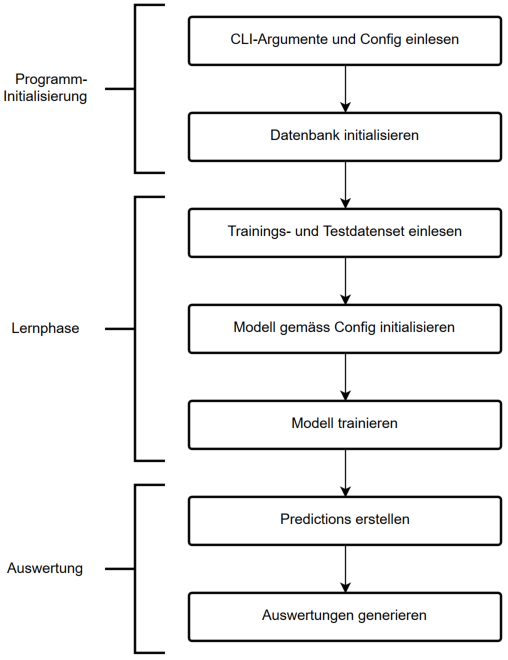
\includegraphics[width=0.7\linewidth]{resources/images/ml_pipeline_flowchart}
\caption[Programmablauf der ML-Pipeline]{Der grobe Programmablauf der ML-Pipeline}
\label{fig:ml_pipeline_flowchart}
\end{figure}

%%% ablauf: %%%

% cli-Argumente und Config einlesen
% Datenbank initialisieren
% Trainings- und Testset einlesen
% Modell gemäss Config initialisieren
% Modell trainieren
% Predictions erstellen
% Auswertungen generieren

Die Projektstruktur ist ähnlich simpel aufgebaut, wie die Abbildung \ref{fig:ml_pipeline_packages} zeigt. Es wurde insbesondere darauf geachtet, die Abhängigkeiten klein zu halten. Der Einstiegspunkt ist das Python-File \emph{ml\_pipeline.py}, welches auch für den Ablauf der Pipeline zuständig ist.
Im Package \emph{utils} ist vor allem das Modul \emph{Config} relevant, welches das externe Konfigurationsfile liest und auch den Zustand der Konfiguration speichert. Dieser Zustand wird ausschliesslich von \emph{ml\_pipeline.py} gelesen und dann über Parameter an die Logik in den anderen Packages weitergegeben. Dadurch wird eine zu grosse Abhängigkeit zu \emph{Config} verhindert.
Das Package \emph{model} enthält die ORM-Objekte und die \ac{DB}-Anbindungslogik. Letztere ist mit der Implementation des Repository Miners grösstenteils identisch. Bei den ORM-Objekten wurden für die ML-Pipeline nicht relevante Attribute aus Effizienzgründen entfernt.
Der grösste Teil der Logik befindet sich im Package \emph{ml}. \emph{Dataset} ist für das Laden und Verarbeiten von Datensets zuständig, \emph{Model} für das Initialisieren und Trainiern der Regressionsmodelle, \emph{Predict} erstellt Model- und Baseline-Predictions und \emph{Reporting} enthält alle Auswertungsfunktionen. 

\begin{figure}[h]
	\centering
	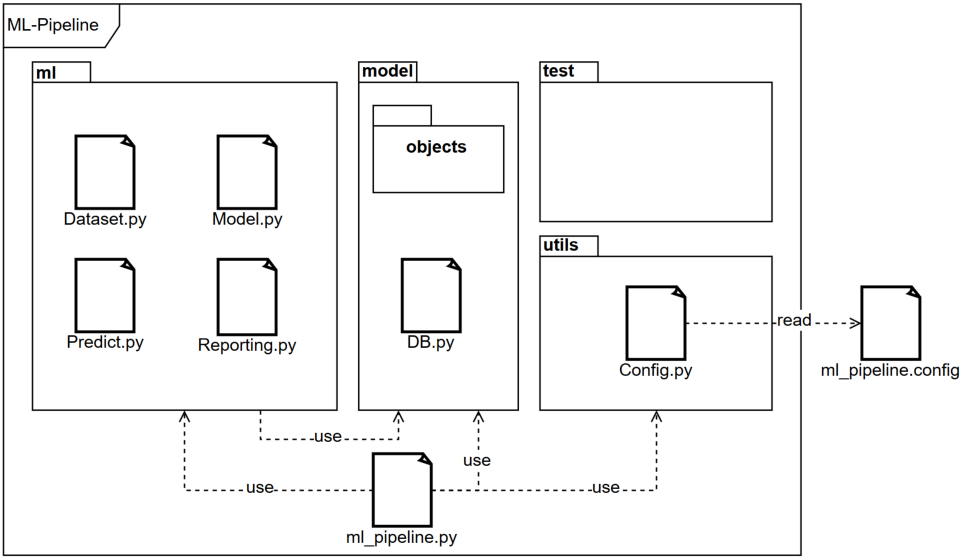
\includegraphics[width=1\linewidth]{resources/images/ml_pipeline_packages}
	\caption[Packages der ML-Pipeline]{Die Package-Struktur der ML-Pipeline (grob vereinfacht)}
	\label{fig:ml_pipeline_packages}
\end{figure}

\subsubsection{Implementierung} \label{sec:ml_pipeline_implementation}
An dieser Stelle wird auf einige hervorzuhebende Probleme und Lösungen in der Implementierung der ML-Pipeline eingegangen.

\paragraph{Datasets} Der Umgang mit den grossen Datenmengen der Trainings- und Testsets war eine der grösseren Herausforderungen bei der Implementation der ML-Pipeline und erforderte diverse Optimierungen. Datensets sind Objekte, die aus 2 Komponenten bestehen, der Data-Matrix (Attribut \emph{data}) und dem Target-Vektor (Attribut \emph{target}). Erstere enthält sämtliche Features aller Versionen im Datenset, wobei jede Zeile der Matrix den Feature-Vektor einer Version darstellt. Das heisst, die Data-Matrix ist immer von der Form \((n_{versions} \times n_{features})\). Der Target-Vektor enthält die Zielwerte, also z. B. die Anzahl Bugfixes pro Monat für jede Version. Er hat die Länge \((n_{versions})\).

Anfangs war das Hauptproblem, dass sich das Einlesen der Features aus der Datenbank als sehr langsam gestaltete. Der Grund dafür war, dass alle Daten über das \ac{ORM} mit Lazy Fetching geladen wurden, was zu einer immens hohen Anzahl von SQL-Queries führte. Der dadurch entstandene Mehraufwand führte zu sehr langen Ladezeiten der Datensets. Als erster Lösungsansatz wurde alles auf Eager Loading umgestellt, was bedeutete, dass alle Daten vom \ac{ORM} über eine grosse Join Query geladen werden. Für kleine Datenmengen war dies sehr effizient, doch für eine grössere Anzahl von Versionen und Features bewährte sich dieser Ansatz nicht. Durch die grossen Joins wurde das Resultat der SQL-Query zu gross für den Arbeitsspeicher. Als Konsequenz wurde Eager Loading für die Features bzw. N-Grams wieder deaktiviert, für die restlichen Tabellen (\emph{Commit}, \emph{Version}, \emph{UpcomingBugsForVersionMv}) wurde es beibehalten. Dies stellte sich als sinnvolle Balance zwischen Rechenzeit und Speicherverbrauch heraus und ermöglichte das Laden sowohl von grossen als auch kleinen Datensets in nützlicher Frist. Bei Bedarf lässt sich Eager Loading aber in der Konfiguration mit dem Parameter \emph{eager\_load} in der Sektion \emph{[DATABASE]} für alle Tabellen aktivieren.

Trotz Optimierungen war die Ladezeit von Datensets hinderlich für die Entwicklung. Aus diesem Grund wurde eine Cache-Funktion für Datensets implementiert. Wenn diese aktiviert ist (über die Einstellung \emph{cache = True} in der Sektion \emph{[DATASET]}) werden Datensets nach dem Einlesen aus der Datenbank in einer Datei gespeichert. Sofern möglich, wird ein menschenlesbares Format gewählt. So muss ein Datenset im Idealfall nur einmal aus der Datenbank gelesen werden und kann ab diesem Zeitpunkt äusserst effizient vom Dateisystem geladen werden. Unterschieden werden die Datensets anhand ihres Dateinamen. Zum Beispiel:

\begin{lstlisting}[breaklines=true,caption={Datenset Dateiname}]
Test_2015_01_01_2015_06_30_sixmonths_ngrams_1-2-3_1-2-3-4_sparse_a773ef13d1f7cd7710dfc2f7efe5532b.datenset
\end{lstlisting}

Diese Datei enthält ein Datenset mit dem Label ``Test'', umfasst den Zeitraum vom 01.01.2015 bis 30.06.2015 und hat als Target die Anzahl Bugfixes in den nächsten 6 Monaten. Sie enthält N-Grams mit der Grösse 1-3 und den Leveln 1-4. Die N-Grams/Features sind als Sparse-Matrizen gespeichert. Der letzte Teil des Dateinamens ist ein MD5-Hash über die Feature-Liste. Eine komplette Auflistung der Features hätte den Dateinamen zu lang gemacht, mit dem Hash können unterschiedliche Feature-Kombinationen dennoch unterschieden werden.

Ein weiteres Problem mit den Datensets trat auf, sobald N-Grams dazugeschaltet wurden und die Anzahl Feature-Werte damit dramatisch stieg. Bei grossen Datensets wurden bis zu 40 GB Arbeitsspeicher benötigt, was zumindest mit unserer Infrastruktur (siehe Kapitel \ref{sec:infrastructure}) nicht mehr bewältigbar war. Da die meisten N-Grams einer Version eine grosse Anzahl von 0 aufweisen, ist die entstehende Data-Matrix eine sogenannte Sparse-Matrix (auch dünnbesetzte oder schwachbesetzte Matrix). \emph{Scipy} bietet im Package \emph{scipy.sparse} eine Auswahl von verschiedenen Speicherformaten für Sparse-Matrizen an, welche diesen Umstand ausnutzen.

Wenn in der Konfiguration der Parameter \emph{sparse} in der Sektion \emph{[DATASET]}) auf True geschaltet ist, wird die Data-Matrix im CSR-Format (Compressed Sparse Row, \emph{scipy.sparse.dok.csr\_matrix}) gespeichert. Dieses Format lässt effizientes Row Slicing sowie arithmetische Operationen zu, wie sie \emph{scikit-learn} benötigt. Der Speicherverbrauch reduziert sich damit immens, nachteilig ist aber, dass gewisse Limitationen beim Preprocessing auftreten. So kann der \emph{StandardScaler} von \emph{scikit-learn}, welcher für das Feature Scaling verantwortlich ist, die Daten einer Sparse-Matrix nicht zentrieren. Auch polynomiale Features sind damit nicht mehr möglich.

Ein weiteres Problem war Anfangs der Aufbau der CSR-Matrix. Strukturänderungen stellten sich als sehr ineffizient heraus, so dass das Einlesen von N-Grams mehrere Stunden dauerte. Als Lösung wurde das Datenset zuerst mit einer DOK-Matrix (Dictionary Of Keys, \emph{scipy.sparse.dok.dok\_matrix}) initialisiert. Diese Datenstruktur erlaubte es die Matrix inkrementell aufzubauen. Wenn alle Daten eingelesen sind, wird die Matrix ins CSR-Format konvertiert. Eine weitere Optimierung war es, 0-Werte nicht in die DOK-Matrix zu schreiben. Dadurch wurde die Datenstruktur zwar nicht grösser (da 0-Werte nicht gespeichert werden), trotzdem benötigte es aber Rechenzeit, vermutlich für den Look-Up in der Matrix. Mit diesen beiden Anpassungen wurde das Einlesen mit N-Grams auch bei grossen Datensets auf wenige Minuten reduziert.

% Datasets:
%% Einlesen der Datensets langsam -> Optimiert mit mix aus lazy und eager loading
%% Einlesen der Datensets langsam -> Cache funktion
%% Speicherbedarf mit NGrams riesig -> Sparse matrizen
%%% Einlesen von Sparse matrizen erst ineffizient, gelöst mit Umwandlung

% Pipelines
\paragraph{Preprocessing und Pipelines} Preprocessing umfasst Transformationen der Data-Matrix, bevor das Modell darauf angepasst wird. Die ML-Pipeline unterstützt Feature Scaling und polynomiale Features (siehe Kapitel \ref{sec:ridgereg}).

Am Anfang der Entwicklung führten wir das Preprocessing manuell auf den Datensets aus, was den Vorteil hatte, dass wir das transformierte Datenset cachen konnten. Es machte aber auch die Logik komplizierter und wir begingen Anfangs den Fehler, dass wir Trainings- und Testset separat skaliert haben, was zu sehr schlechten Ergebnissen führte.

Es stellte sich heraus, dass \emph{scikit-learn} mit Pipelines eine simple und effiziente Lösung bietet. Pipelines können benutzt werden, um mehrere Estimators aneinanderzuketten und diese dann wie ein normales Modell benutzen zu können. \cite{sklearnpipelines} Als Estimator gelten sowohl Preprocessing-Komponenten als auch\ac{ML}-Modelle. Allerdings müssen zwingend alle Schritte bis auf den letzten Transformatoren sein, d. h. sie müssen über eine transform()-Methode verfügen.

Pipelines lassen sich sehr einfach konstruieren:

\begin{lstlisting}[language=Python, frame=single,caption={Python Pipeline Code}]
from sklearn import svm
from sklearn.pipeline import Pipeline
from sklearn.preprocessing.data import PolynomialFeatures
from sklearn.preprocessing.data import StandardScaler

scaler = StandardScaler()
poly = PolynomialFeatures(degree=2)
svm = svm.SVR(kernel='linear', C=0.1)

steps = [('scale', scaler), ('poly', poly), ('svr', svm)]

model = Pipeline(steps=steps)	
\end{lstlisting}

Der Vorteil ist, dass auf dem konstruierten Pipeline-Modell nur noch einmal fit() und predict() aufgerufen werden muss. Der Scaling-Faktor des StandardScalers wird automatisch gespeichert und beim Aufruf von predict() auf das Input-Datenset angewendet.
Ausserdem ermöglichen es Pipelines auch, Grid Search über alle Parameter der Komponenten in einem Lauf durchzuführen.

\paragraph{Predicting} Neben der Vorhersage mit Hilfe eines trainierten Modells kann die ML-Pipeline noch drei verschiedene Baseline-Predictions erstellen. Diese sollen als naive Vergleichswerte für die Performance des Modells dienen:
\begin{enumerate}
	\item \textbf{Mean Prediction}: Ein konstantes Modell, welches unabhängig vom Inputwert den arithmetischen Mittelwert des Target-Vektors des Trainingssets zurückgibt.
	
	\item \textbf{Median Prediction}: Ein konstantes Modell, welches unabhängig vom Inputwert den Median des Target-Vektors des Trainingssets zurückgibt.
	
	\item \textbf{Weighted Random Prediction}: Dieses Modell bezieht aus dem Trainingsset die Verteilung der Werte des Target-Vektors. Es wählt die Rück\-gabe\-werte zufällig, wobei häufige Werte aus dem Trainingsset-Target mit einer entsprechend höheren Wahrscheinlichkeit gewählt werden.	
\end{enumerate}

\paragraph{Reporting} Das Re\-port\-ing-Modul (\emph{ml.Reporting}) bietet verschiedene Mög\-lich\-kei\-ten zur Auswertung eines Modells an. Folgende Reports werden, in ASCII-Tabellen formatiert und in schriftlicher Form ausgegeben respektive in einer Textdatei gespeichert:
\begin{itemize}
	\item \textbf{Config}: Alle relevanten Parameter aus der Konfiguration werden aufgelistet. Das ist wichtig um die Übersicht zu behalten und Resultate den jeweiligen Einstellungen zuordnen zu können.
	
	\item \textbf{Regressionsmetriken}: Über die Klasse \emph{ml.Reporting.Report} können alle im Kapitel \ref{sec:regressionmetrics} beschriebenen Metriken erstellt werden. Diese können anschliessend nicht nur in Tabellenform ausgegeben, sondern mit der Funktion \emph{get\_report\_comparisation\_table} auch einfach miteinander verglichen werden. Das ist insbesondere sinnvoll um die Scores der Baseline, des Trainingsets und des Testsets gegenüberzustellen.
	
	\item \textbf{Top-Features}: Die Funktion \emph{get\_top\_features\_table} listet die am Höchsten gewichteten Features des trainierten Modells auf. Das lässt sich nur auf lineare Regression, Ridge Regression und \ac{SVR} mit linearem Kernel anwenden, da die Gewichtung von anderen \ac{SVR} Kernelfunktionen verzerrt wird. Auch mit polynomialen Features macht dieser Report keinen Sinn, da die entstehenden Polynome nicht mehr den ursprünglichen Features zugeordnet werden können. Am Anfang der Entwicklung der ML-Pipeline war dieser Report aber sehr praktisch, da auffällige Feature-Gewichtungen auf Fehler hindeuteten.
	
	\item \textbf{Kategorische Auswertung}: In der angedachten Anwendung eines Feh\-ler\-vor\-her\-sa\-ge-Tools ist ein kontinuierlicher Wert für den Benutzer vermutlich uninteressant, da es schliesslich keine ``halben'' Bugs gibt. Vielmehr würde er eine diskrete Auswertung erwarten. Aus diesem Grund wurde die Funktion \emph{get\_category\_table} implementiert. Sie bildet die kontinuierlichen Vorhersagen eines Modells auf beliebige Kategorien ab, z. B. 0 Bugs, 1 Bug, 2-3 Bugs und 4+ Bugs. Für jede Kategorie werden die Anzahl richtiger und falscher Aussagen der Vorhersage gezählt. Das erlaubt eine realitätsnähere Auswertung des Modells.
	
	\item \textbf{Confusion-Matrize}: Da sich die kategorische Auswertung bewährte, wurde für eine detailliertere Auswertung eine Confusion-Matrix (auch \emph{Error Matrix} \cite{Stehman1997}) implementiert. Sie wird oft bei (Multi-) Klas\-si\-fi\-ka\-tions\-pro\-b\-lemen verwendet. Jede Spalte der Matrix repräsentiert eine Vorhersageklasse, die Zeilen sind die Klassen der Ground Truth. Damit stellt die Diagonale der Matrix die Anzahl korrekter Vorhersagen dar. Im Gegensatz zur kategorischen Auswertung lässt sich zusätzlich auch ablesen, in welchen Klassen die falschen Aussagen gefallen sind. Sie lässt sich mit der Funktion \emph{get\_confusion\_matrix} generieren.
	
	\item \textbf{Classification Report}: Die Funktion \emph{get\_confusion,\_matrix} gibt neben der Confusion-Matrix auch einen Classification Report aus. Denn dank der kategorischen Auswertung ist es auch möglich, die Precision und den Recall pro Kategorie zu bestimmen und damit auch einen F1-Score zu berechnen. Dieser Score wird oft bei Klassifikationsproblemen benutzt, da er es erlaubt, die Qualität einer Vorhersage an einem einzigen Wert abzulesen.
	
	\item \textbf{Ranking}: Um verschiedene Reports zu vergleichen, wurde ausserdem das Modul \emph{ml.Scoreboard} implementiert. Dieses speichert die Resultate eines ML-Pipeline-Durchlaufs zusammen mit dessen Konfiguration in einer Datei. Wird diese später wieder ausgelesen, kann der aktuelle Lauf mit den vergangenen Läufen anhand einer beliebigen Metrik verglichen werden. Da diese Auswertung nicht idempotent ist und ohne Kontext der vorherigen Durchläufe nicht aussagekräfig ist, wird in dieser Arbeit nicht weiter darauf eingegangen. Sie stellte sich aber während dem Testen und Entwickeln einige Male als nützlich heraus.
\end{itemize}

\subsubsection{Erkenntnisse}

Die ML-Pipeline entwickelte sich zu einer leistungsfähigen Software, welche vergleichsweise einfach zu bedienen ist. Durch die einfache aber umfangreiche Konfigurationsmöglichkeit und die Performance-Features ermöglicht sie, Experimente vielseitig zu gestalten.

Als nachteilig erwies sich, dass neue Funktionen nicht ganz so einfach ergänzt werden können, wie wir es uns gewünscht haben, da sie zuerst in den bestehenden Aufbau eingegliedert werden müssen. Oft verlangte dies Anpassungen beim Einlesen der Konfiguration oder auch beim Datenset-Caching (da neue Attribute in die Logik aufgenommen werden müssen). Wirkliches Rapid Prototyping hätte man erreicht, indem man direkt mit \emph{scikit-learn}-Skripts gearbeitet hätte. Parameteranpassungen bei Experimenten wären dadurch allerdings wesentlich aufwändiger geworden.

Weitere Probleme betreffen Performance und Skalierbarkeit. Beides ist mit dem jetzigen Design und der Python-Plattform limitiert. Für den Rahmen dieser Arbeit sind aber sowohl die aktuelle Performance als auch die Skalierbarkeit hinreichend.
% Nachteile:
%% Rapid Prototyping nicht mehr so gut möglich, da wäre einfach sklearn einfacher. Ging zugunsten von einfacher Konfigurierbarkeit
%% Performance
%% Scalability



% Mit nGrams:
%% Das Problem wo de Egger beschäftigt:
%% Problem: Annahme: Code File mit seltenen ngrams, welche aber nichts mit einem Bug / Bugfix zutun haben. Dieses File ist anschliessend von Bugs betroffen. Der Computer assoziert dann die selten vorkommenden ngrams mit einem Bugfix und gewichtet diese hoch. --> Das könnte ein Problem werden.
\subsection{Machine Learning} \label{sec:approach_ml}

Ob der von uns verfolgte Ansatz funktioniert, zeigte sich in diversen \ac{ML}-Ex\-pe\-ri\-menten. In diesem Kapitel sollen die Vorgehensweise und die Überlegungen zu diesen Versuchen beschrieben werden.

Da reale Projekte als Datenbasis dienten, stellte sich die Frage, wie die Fehlervorhersage validiert werden soll. Eine Möglichkeit wäre gewesen, ein Trai\-nings- und Testset aus einer zufälligen Auswahl von Dateiversionen  zusammenzustellen. Am Sinnvollsten erschien es uns aber, das Trainings- und Testset zeitlich aufzuteilen. Dies richtet sich an den angedachten Anwendungsfall, in dem ein Tool aus einer bestimmten Zeitspanne der Vergangenheit lernt und dann Voraussagen für die Zukunft machen wird. Ein Beispiel soll dies verdeutlichen:

Als Trainingszeitraum wird der 01.08.2014 bis 31.12.2014 verwendet. Auf dem Trainingsset gewichtet der \ac{ML}-Algorithmus die einzelnen Features um dann anschliessend Bug-Vorkommnisse für das nächste halbe Jahr zu prognostizieren. Eine zweite, etwas kürzere Zeitspanne, zum Beispiel 01.01.2015 bis 31.01.2015, wird als Testset verwendet. Da auch das Testset in der Vergangenheit liegt, ist die Anzahl Bugs bereits bekannt. Dieser Wert dient als Ground Truth, mit welcher die Vorhersage des \ac{ML}-Modells verglichen wird. Die Abbildung \ref{fig:ml_experiment_phases} soll das Beschriebene verdeutlichen.

\begin{figure}[h]
	\centering
	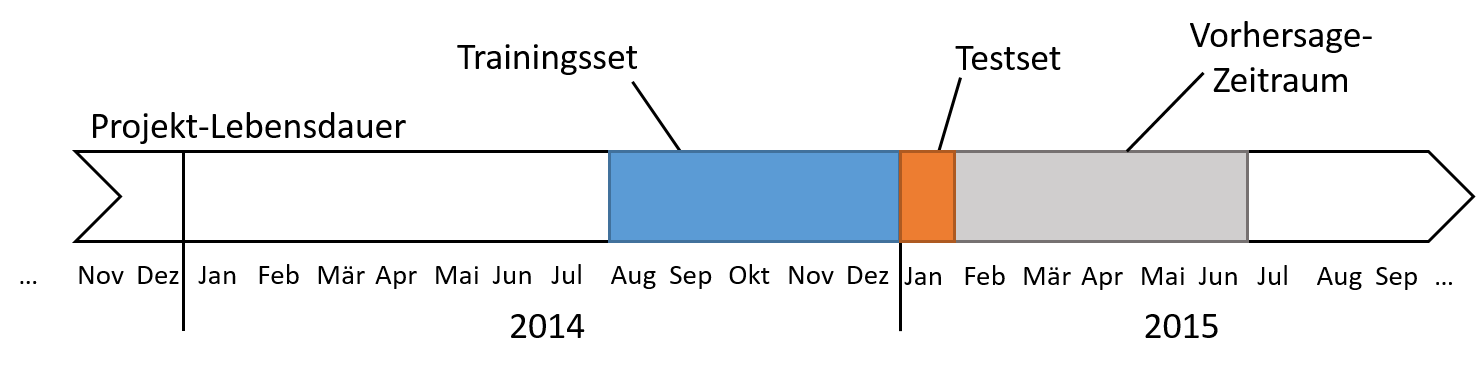
\includegraphics[width=1\linewidth]{resources/images/ml_experiment_phases.png}
	\caption{Phasen der ML-Experimente}
	\label{fig:ml_experiment_phases}
\end{figure}

Um eine repräsentative Aussage über die Leistung des Toolsets und der verwendeten Features machen zu können, sind eine grosse Anzahl an Experimenten notwendig. Aufgrund des Zeitplans war es uns nicht möglich, Experimente in diesem Umfang durchzuführen. Stattdessen verglichen wir mithilfe einer kleine Auswahl an Experimenten die Performance der verschiedenen \ac{ML}-Modelle miteinander. Insbesondere sollte geprüft werden, ob die von uns definierten Baselines (siehe Kapitel \ref{sec:mlpipeline}) übertroffen werden können. Damit wollten wir untersuchen ob das in dieser Arbeit beschriebene Verfahren ansatzweise funktioniert und welche Algorithmen die besten Ergebnisse liefern.

Ausserdem wurden die Effektivität der einzelnen Feature-Gruppen analysiert. Dazu wurden bei identischer Konfiguration einzelne Feature-Gruppen deaktiviert und geprüft, wie sich dadurch die Vorhersagen ändert (sog. Ablation-Tests).

\paragraph{Gemeinsame Parameter} Die gemeinsamen Parameter der Versuche werden in Tabelle \ref{tab:ml_experiments_parameter} aufgeführt.

\begin{table}[h]
	\begin{tabular}{rl}
	\hline
	Zeitraum Traingsset:		& 01.10.2014 - 31.12.2014	\\
	Zeitraum Testset:		& 01.01.2015 - 31.01.2015 	\\
	Repository:					& \emph{Elasticsearch}	\\
	Cross Validation:			& Ja	\\
	Ridge Regression \(\alpha\):& 1, 0, 0.01, 0.1, 10, 100, 1000	\\
	\acs{SVR} \(C\):			& 1, 0.001, 0.01,  0.1, 5, 10, 50, 100	\\
	\acs{SVR} \(\epsilon\):		& 0.1	\\
	\acs{SVR} \(\gamma\):		& auto	\\
	\acs{SVR} \emph{degree}:	& 3	\\
	\acs{SVR} \emph{coef0}:		& 0	\\
	\hline
	\end{tabular}
	\centering
	\caption{Parameter der ML-Experimente}
	\label{tab:ml_experiments_parameter}
\end{table}

Die Trainingszeiträume von uns sind so ausgewählt worden, dass sie in vernünftiger Zeit terminieren. Die Laufzeit hängt natürlich von den gewählten Parametern (vor allem dem ML-Algorithmus, mit/ohne N-Grams und \ac{CV}) ab.

\section{Resultate}
% (Zusammenfassung der Resultate)

In diesem Kapitel werden die Resultate aller relevanten Experimente und deren Auswertungen aufgelistet und beschrieben. Auf die beim Repository Mining gewonnenen Erkenntnisse wird im Kapitel \ref{sec:statistics} eingegangen, das Kapitel \ref{sec:ml_results} behandelt die Resultate der Versuche mit der \ac{ML}-Pipeline.

\subsection{Testdaten}
Als Basis der nachfolgenden Experimente und Auswertungen diente das Softwareprojekt \emph{Elasticsearch} \cite{elasticsearchhomepage}, welches auch anderweitig als primäre Datenquelle für diese Arbeit diente.

\emph{Elasticsearch} ist ein auf \emph{GitHub} gehosteter open-source Search-Engine-Server \cite{elasticsearchgithub} auf Basis von \emph{Apache Lucene}. Das Java-Projekt wird seit Februar 2010 \cite{elasticsearchrelease} von Shay Banon als Hauptentwickler gepflegt und steht unter der Apache License. Es ermöglicht das Durchsuchen von beliebigen Dokumenten (fast) in Echt\-zeit über ein verteiltes System von Indizes und unterstützt Features wie Multitenancy und eine extensive \acs{REST}- und Java-\acs{API}. \emph{Elasticsearch} ist die momentan meistverbreitetste Enterprise Search Engine \cite{dbsearchengineranking} und wird unter anderem von 
\emph{Wikimedia}		\cite{elasticsearchinwikimedia}, 
\emph{GitHub}			\cite{elasticsearchingithub}, 
\emph{Stack Exchange}	\cite{elasticsearchinstackexchange}, 
\emph{Netflix}			\cite{elasticsearchinnetflix} und
\emph{Sound\-Cloud}		\cite{elasticsearchinsoundcloud}
genutzt.

Damit ist \emph{Elasticsearch} nicht nur allgemein ein spannendes Projekt, es hat sich auch wegen seines Alters (über 6 Jahre), seiner Projektgrösse (ca. 20'000 Commits) und seinem gut gepflegten Issue-Tracking (ca. 10'000 Issues auf \emph{GitHub}) ideal als Testprojekt für diese Arbeit angeboten.

\subsection{Repository Mining} \label{sec:statistics}

Im folgenden Kapitel versuchten wir, mit statistischen Mitteln erste Erkenntnisse zu gewinnen und ein Gefühl für die gesammelten Daten zu erhalten. Dabei eröffneten sich nicht nur interessante Einblicke in die Projektstruktur von \emph{Elasticsearch}, es gelang auch bereits erste Korrelationen zum Auftreten von Bugs zu erkennen.

\subsubsection{Projektstatistiken} \label{sec:project_statistics}

\begin{figure}[!ht]
	\centering
	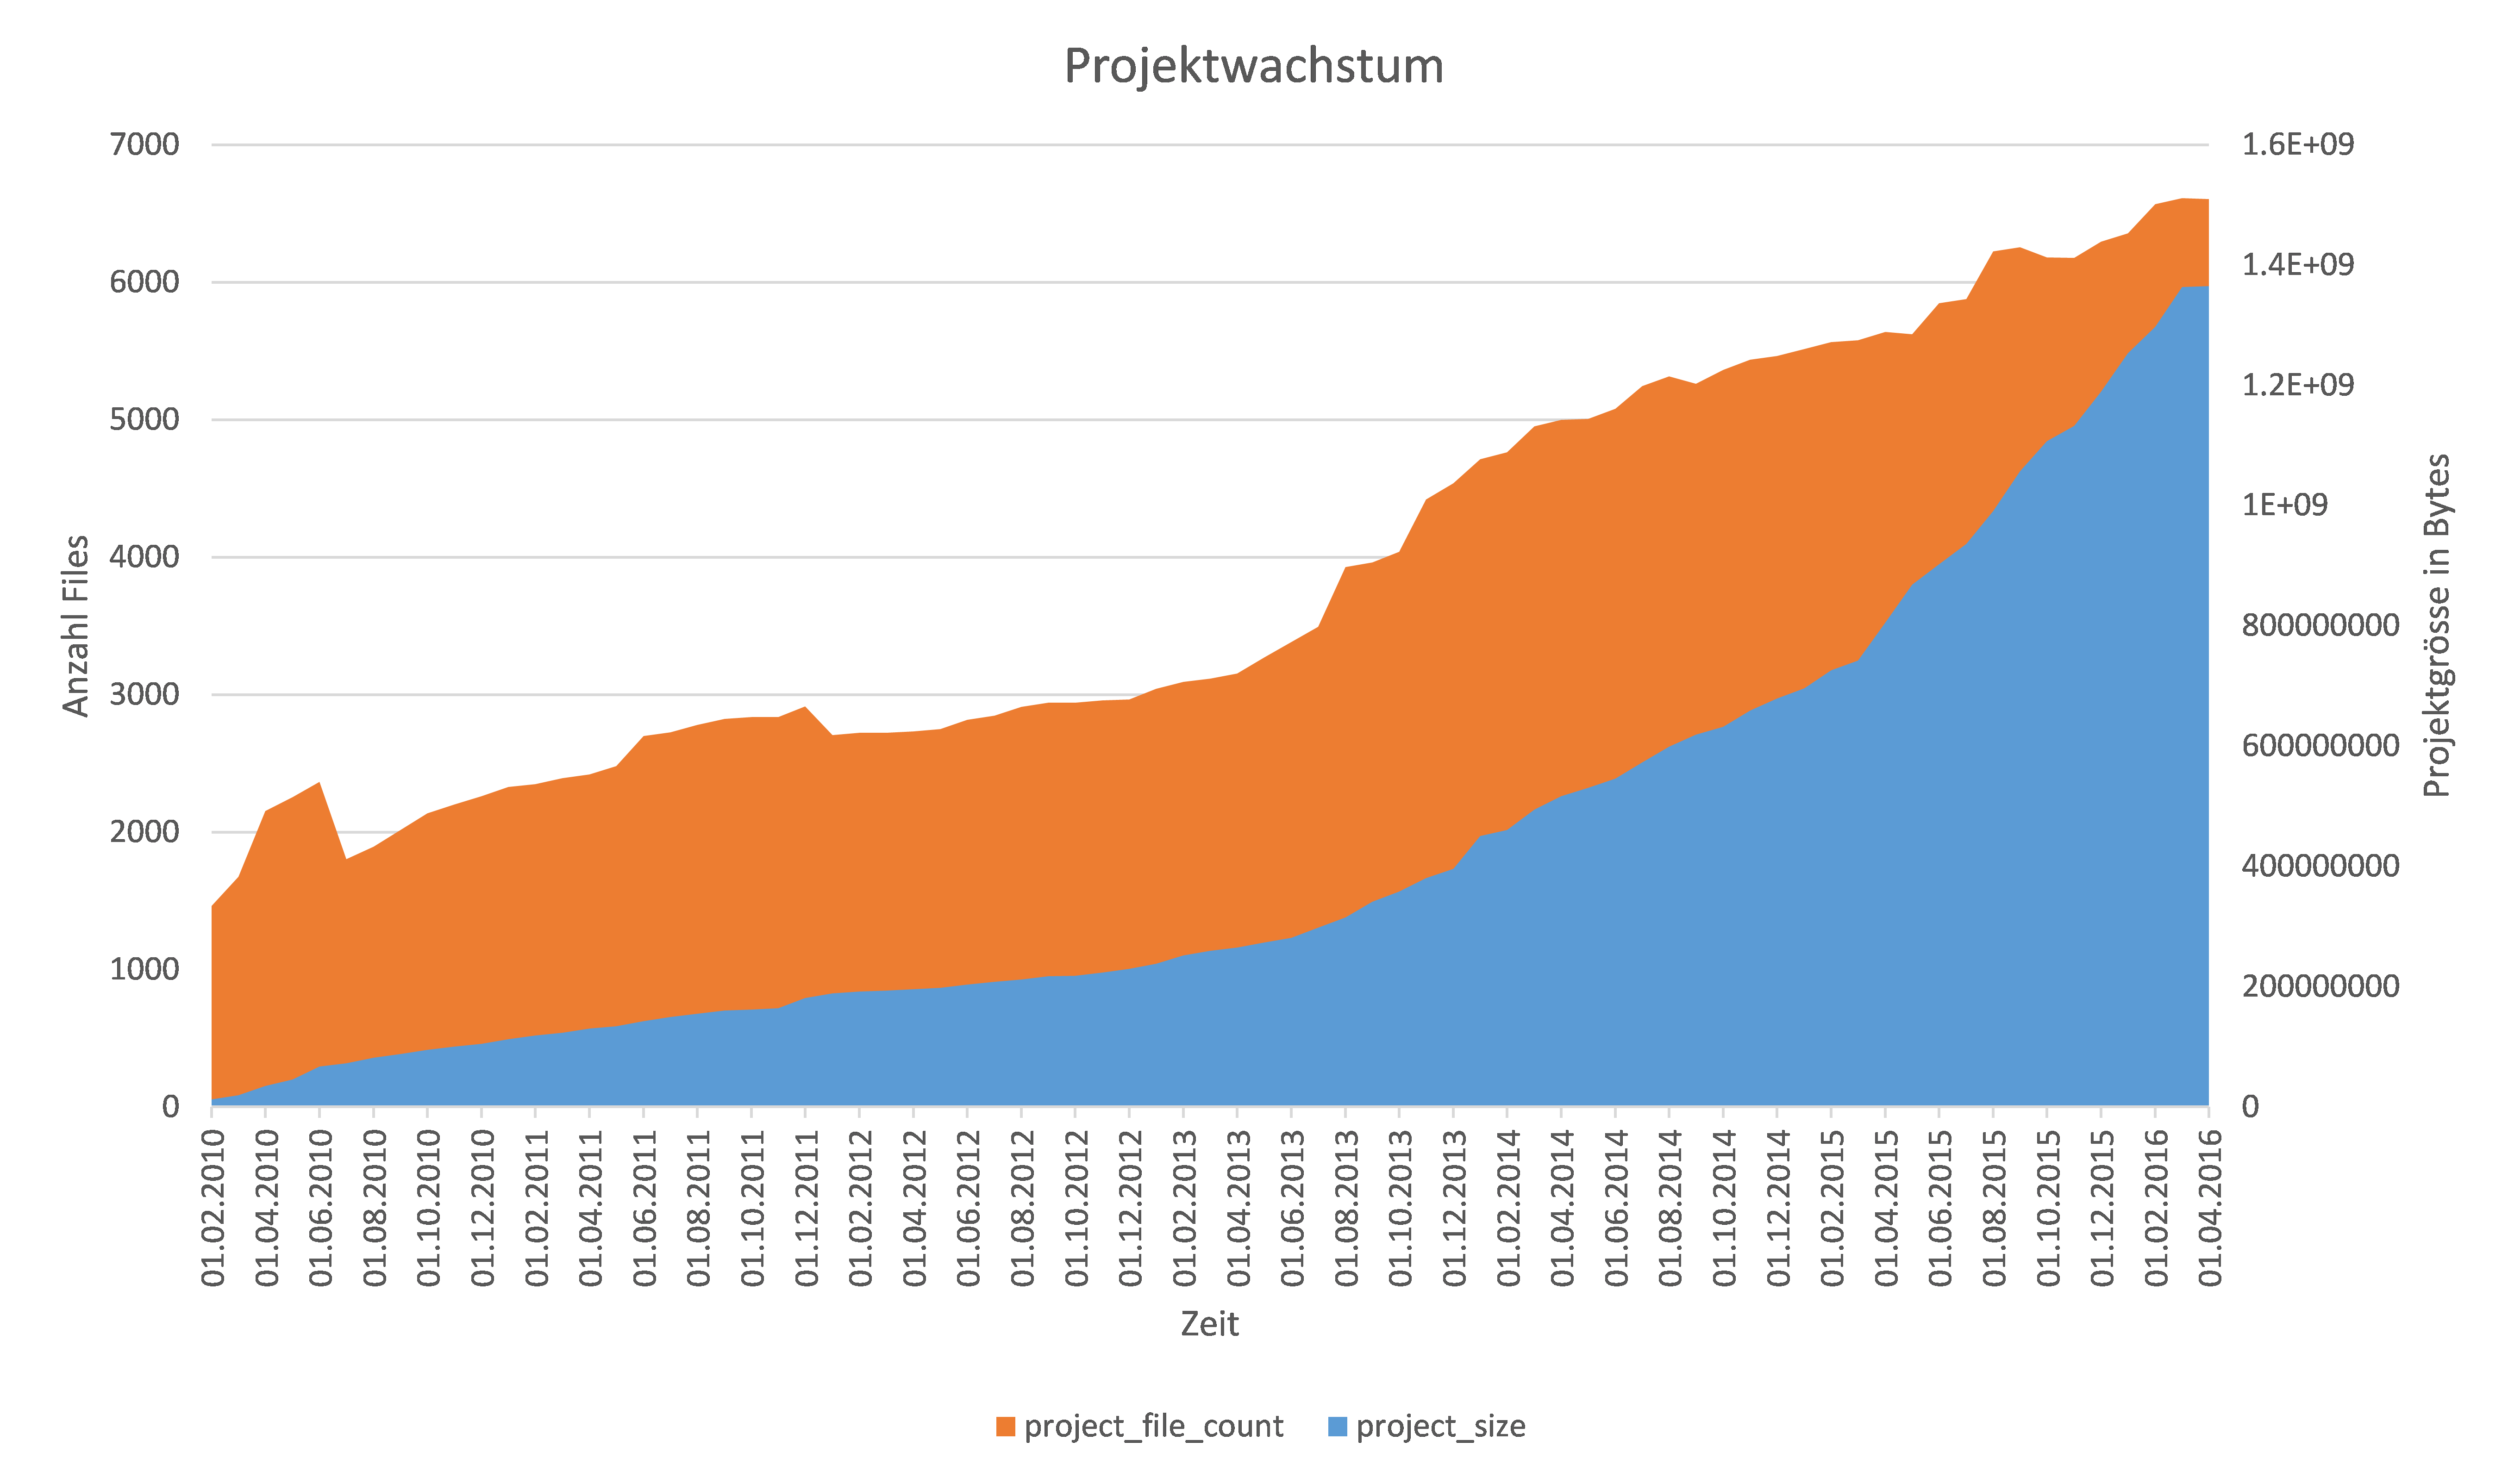
\includegraphics[width=1\textwidth]{resources/images/chart_project_growth.png}
	\caption{Projektgrösse von \emph{Elasticsearch} über die Zeit}
	\label{fig:projectgrowth}
\end{figure}

\begin{figure}[!ht]
	\centering
	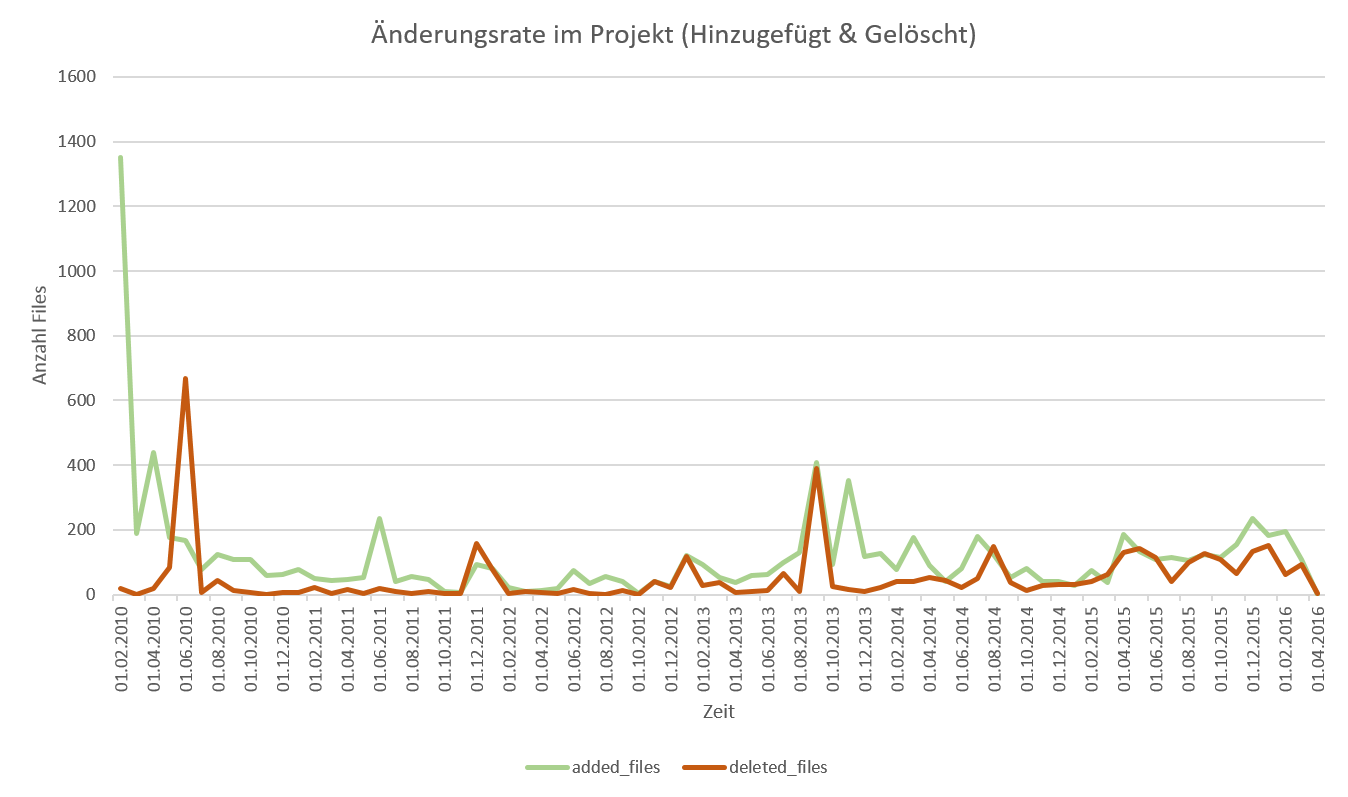
\includegraphics[width=1\textwidth]{resources/images/chart_project_change_rate_1.png}
	\caption{Anzahl hinzugefügter/gelöschter Files im Projekt \emph{Elasticsearch} über die Zeit}
	\label{fig:addeddeletedfiles}
\end{figure}

\begin{figure}[!ht]
	\centering
	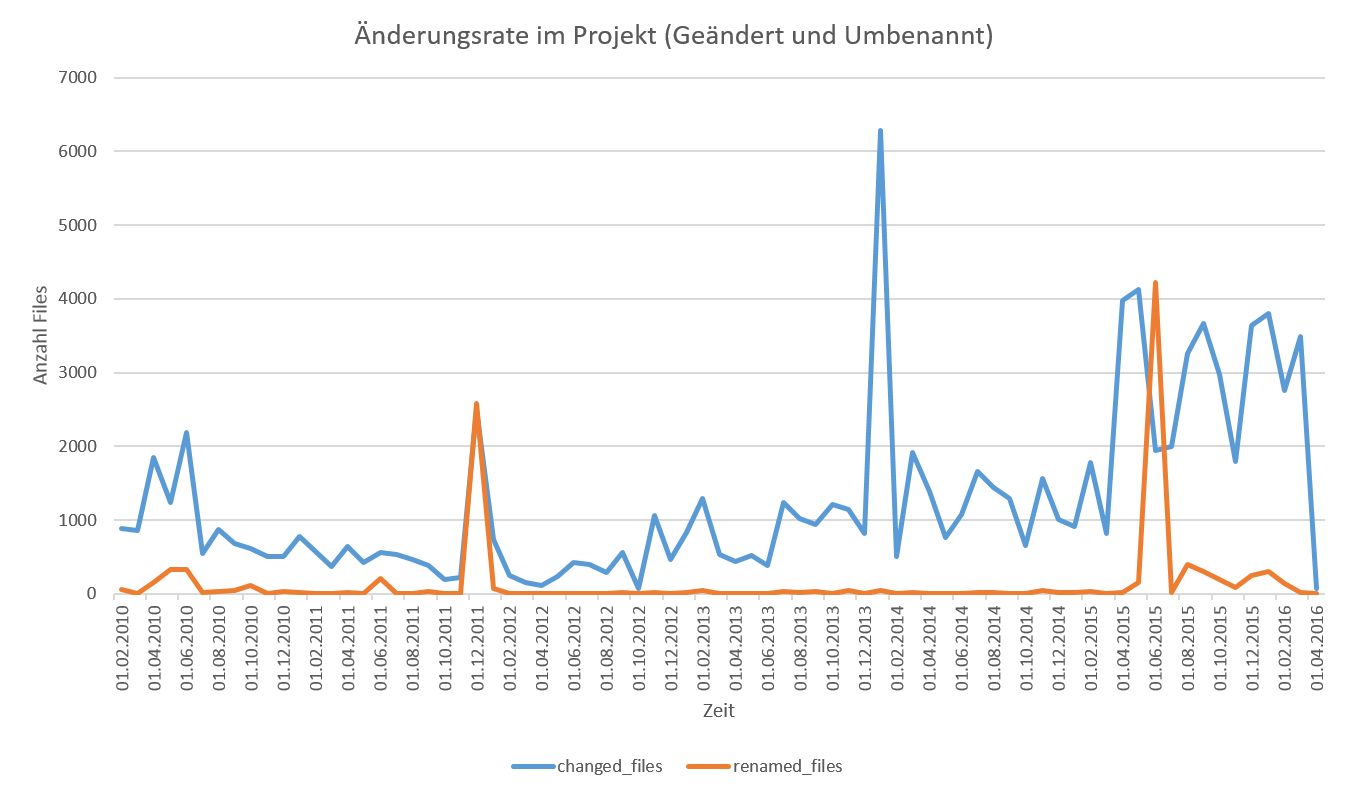
\includegraphics[width=1\textwidth]{resources/images/chart_project_change_rate_2.png}
	\caption{Anzahl geänderter/umbenannter Files im Projekt \emph{Elasticsearch} über die Zeit}
	\label{fig:changedrenamedfiles}
\end{figure}

\paragraph{Projektwachstum} Abbildung \ref{fig:projectgrowth} zeigt, wie das \emph{Elasticsearch}-Projekt seit seiner Entstehung gewachsen ist. Zu erkennen ist hier, dass der initiale Commit am 01.02.2010 bereits ca. 1400 Files hunzugefügt hat. Dieser Initial-Commit fand gerade mal eine Woche vor dem offiziellen Release \cite{elasticsearchrelease} statt, deshalb ist anzunehmen, dass Shay Banon eine bereits lauffähige Version in das heute benutzte \emph{Git}-Repository lud. Solch grosse Initial-Commits lassen sich auch in anderen Projekten beobachten.

Ebenfalls auffällig ist, dass Anfangs die Projektgrösse, also der benötigte Speicherplatz, ungefähr proportional zur Anzahl Files wächst. Ab Anfang 2015 steigt die Projektgrösse allerdings deutlich schneller an, als die Anzahl Files. Vermutlich heisst das, dass ab dieser Zeit vermehrt bestehende Klassen erweitert anstatt Neue erstellt wurden. Die Analyse von File-Stichproben im Kapitel \ref{sec:filesamplestatistics} unterstützt diese Vermutung.

Zuletzt lassen sich in den Abbildungen \ref{fig:addeddeletedfiles} und \ref{fig:changedrenamedfiles} auffällige Spitzen feststellen. Diese zeigen grössere Refactorings und Umstellungen an Core-Komponenten an. Ebenfalls interessant ist, dass sich die Anzahl der geänderten Files mit der Zeit erhöht. Das deutet darauf hin, dass Änderungen mit der Zeit immer mehr Files beeinflussen, möglicherweise durch mehr Abhängigkeiten. Die Anzahl geänderter Files steigt signifikant Anfang 2015, also zeitgleich wie der Anstieg des Projektgrössen-Wachstums.

\begin{figure}[!ht]
	\centering
	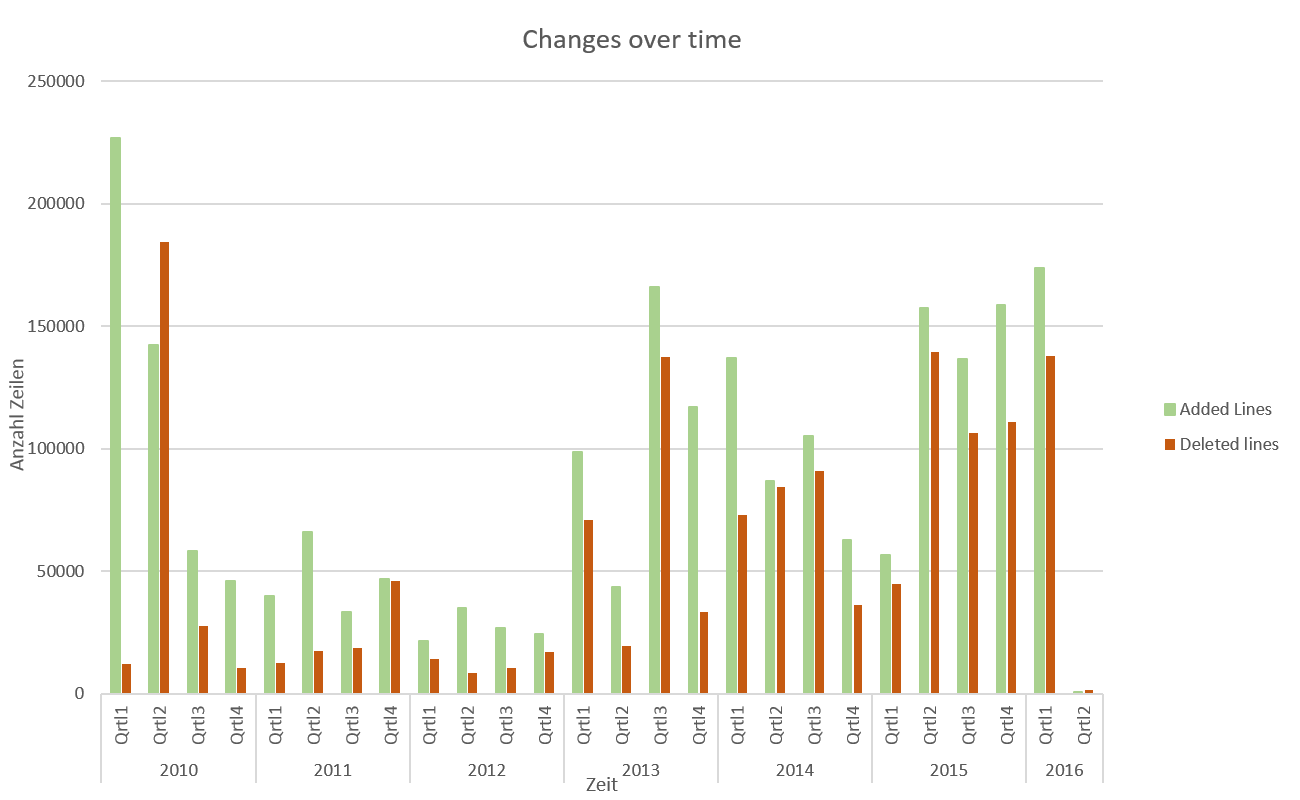
\includegraphics[width=1\textwidth]{resources/images/chart_changed_lines_over_time.png}
	\caption{Anzahl geänderter Zeilen im Projekt \emph{Elasticsearch} über die Zeit}
	\label{changedlinesovertime}
\end{figure}

\paragraph{Zeilenänderungen}
In Abbildung \ref{changedlinesovertime} wird die Menge an total hinzugefügten und gelöschten Zeilen dargestellt. Gut erkennbar ist, dass beide Werte einigermassen proportional zueinander sind. Das war auch zu erwarten, insbesondere da in \emph{Git} eine Zeilenänderung sowohl als gelöschte Zeile (die Zeile im alten Zustand) sowie auch als hinzugefügte Zeile (die Zeile im neuen Zustand) zählt.
Ebenfalls zu erkennen ist, dass durchgehend mehr Zeilen hinzugefügt als gelöscht werden, was zum bereits beschriebenen Projektwachstum führt.

\begin{figure}[!ht]
	\centering
	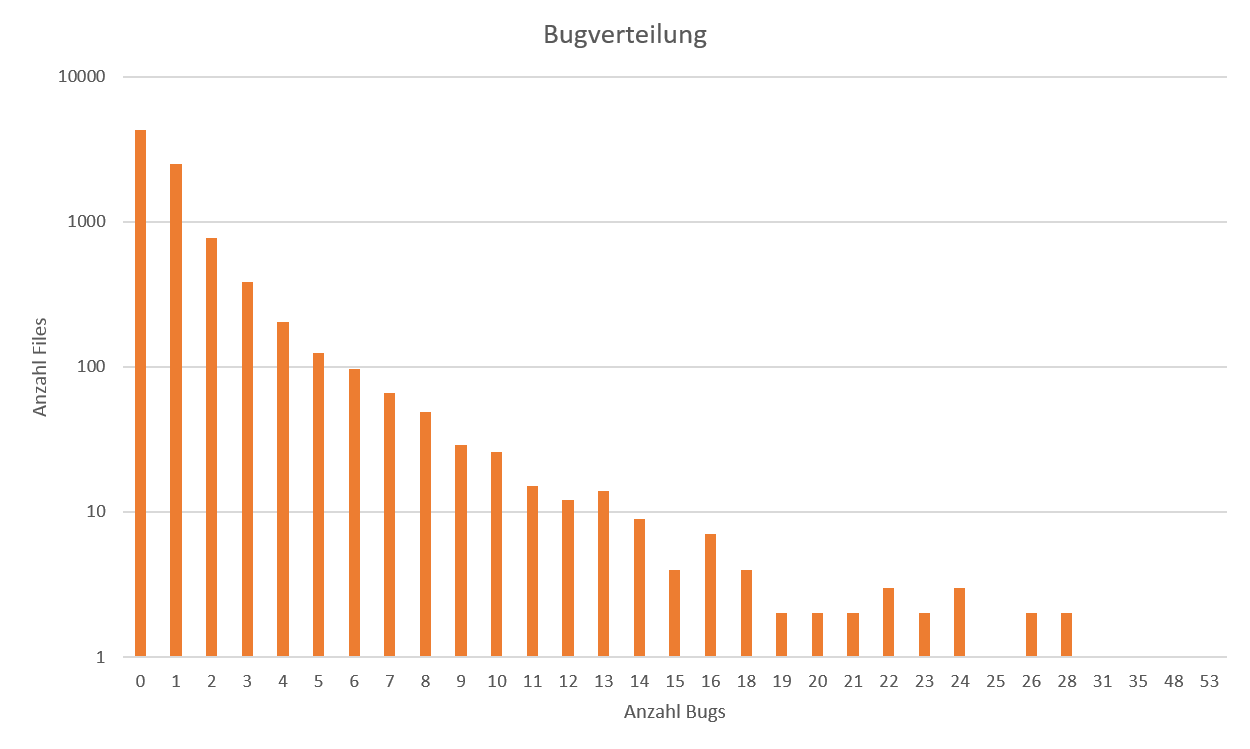
\includegraphics[width=1\textwidth]{resources/images/chart_bug_distribution.png}
	\caption{Anzahl Files pro Anzahl Bugs}
	\label{fig:filecountperbugs}
\end{figure}

\begin{table}[!ht]
	\begin{tabular}[c]{|r|l|}
		\hline
		\textbf{Anzahl Bugs} & \textbf{Anzahl Files} \\
		\hline
		0 & 4265\\
		1 & 2487\\
		2 & 774\\
		3 & 384\\
		\vdots & \vdots \\
		53 & 1 \\
		\hline
		\textbf{Total} & 8593 \\
		\hline
	\end{tabular}
	\centering
	\caption{Auszug von Anzahl Files pro Anzahl Bugs}
	\label{tab:filecountperbugs}
\end{table}

\begin{table}[!ht]
	\begin{tabular}[c]{|r|l|}
		\hline
		\textbf{Total Files} & 8593 \\
		\hline
		\textbf{Total Bugs} & 10043 \\
		\hline
		\textbf{Durchschnitt} & 1.17 Bugs/File \\
		\hline
		\textbf{Median} & 1 Bug \\
		\hline
	\end{tabular}
	\centering
	\caption{Anzahl Bugs zusammengefasst}
	\label{tab:filecountperbugs_summary}
\end{table}

\paragraph{Bugverteilung über Files} Abbildung \ref{fig:filecountperbugs} stellt die Verteilung von Bugs über die gesamte Lebenszeit über alle Java Files dar. Zu beachten ist, dass die Y-Achse (Anzahl Files) logarithmisch skaliert ist. Als Bug gilt jede Änderung, die ein File erfahren hat, welche über das Issue-Tracking mit einem Bug-Issue in Verbindung gebracht wurde.

Tabelle \ref{tab:filecountperbugs} zeigt einen Auszug der gesammelten Daten. Insgesamt umfasst die Statistik 8593 Java-Files aus dem \emph{Elasticsearch}-Projekt. Davon werden 4265 Files, also 49.6\%, nie mit einem Bug in Verbindung gebracht. Von den restlichen 50.4\% aller Files sind wiederum 58.3\% im Zuge eines Bugfixes geändert worden. Files mit über 10 Bugs in ihrer Lebenszeit sind in diesem Projekt äusserst selten, sie machen gerade mal 1.33\% aller Java-Files aus. Im Durchschnitt fallen 1.17 Bugs auf ein File, der Median liegt bei einem Bug.

\begin{figure}[!ht]
	\centering
	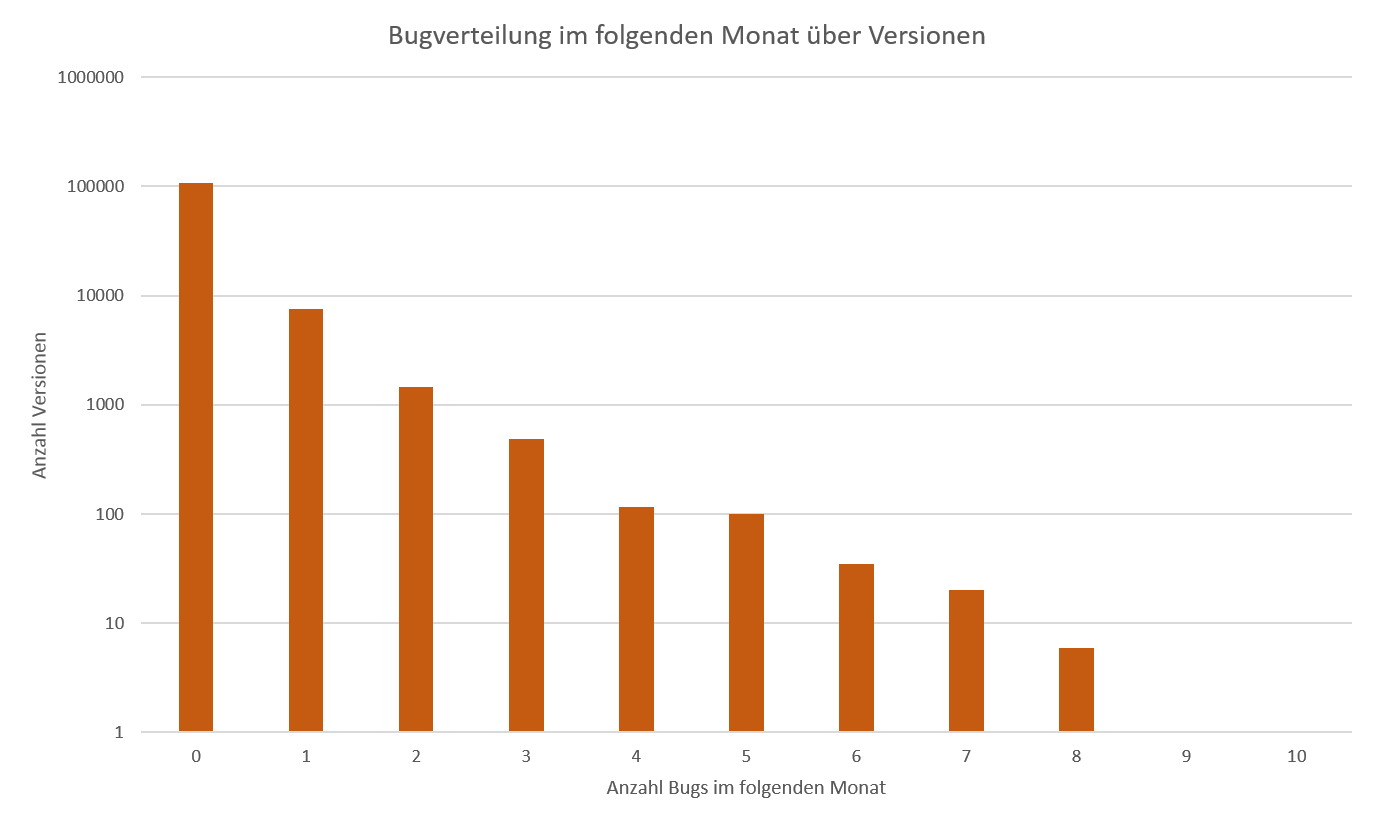
\includegraphics[width=1\textwidth]{resources/images/chart_bug_distribution_1month.png}
	\caption{Anzahl Versionen pro Anzahl Bugs im folgenden Monat}
	\label{fig:versionbugdist_1month}
\end{figure}

\begin{figure}[!ht]
	\centering
	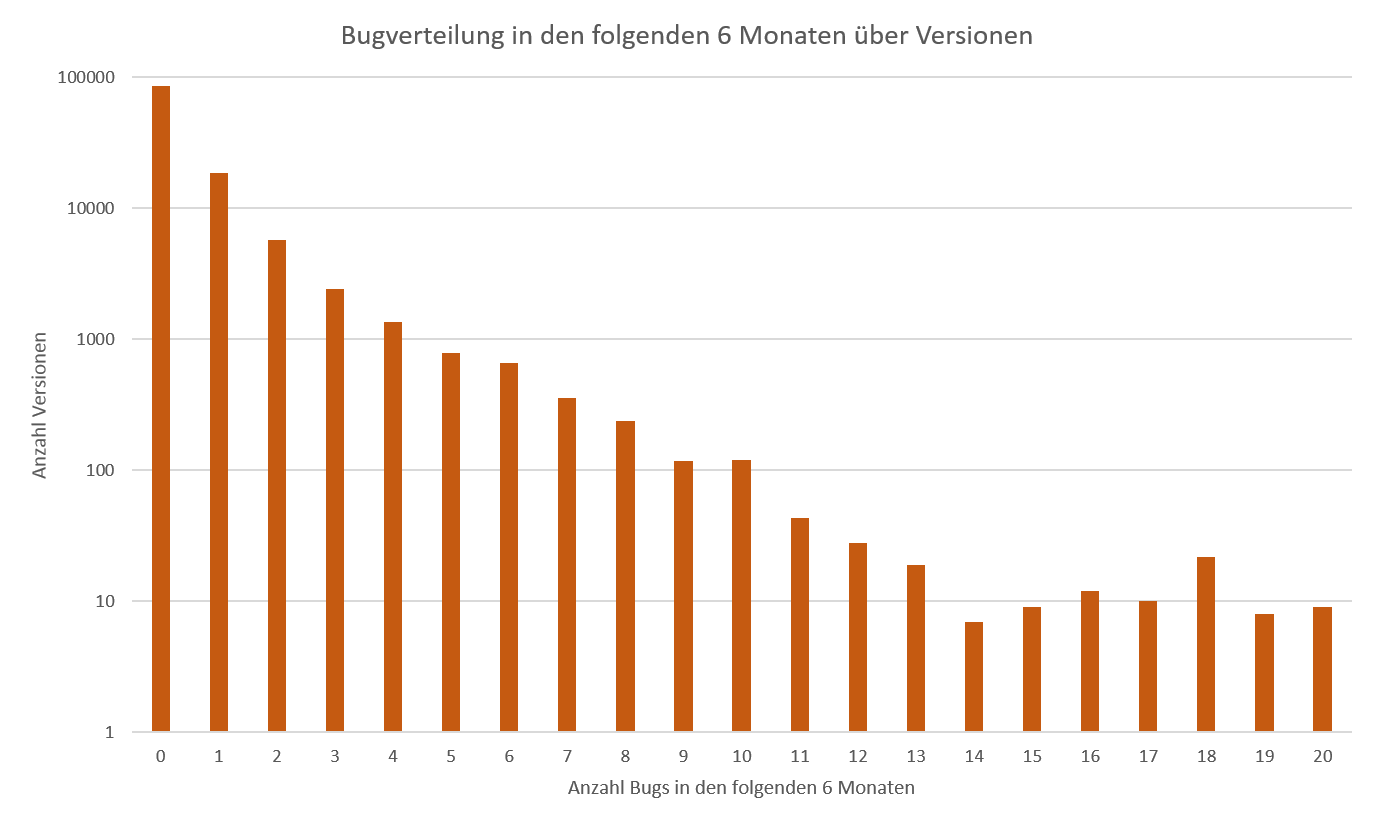
\includegraphics[width=1\textwidth]{resources/images/chart_bug_distribution_6month.png}
	\caption{Anzahl Versionen pro Anzahl Bugs in den folgenden 6 Monaten}
	\label{fig:versionbugdist_6month}
\end{figure}

\begin{figure}[!ht]
	\centering
	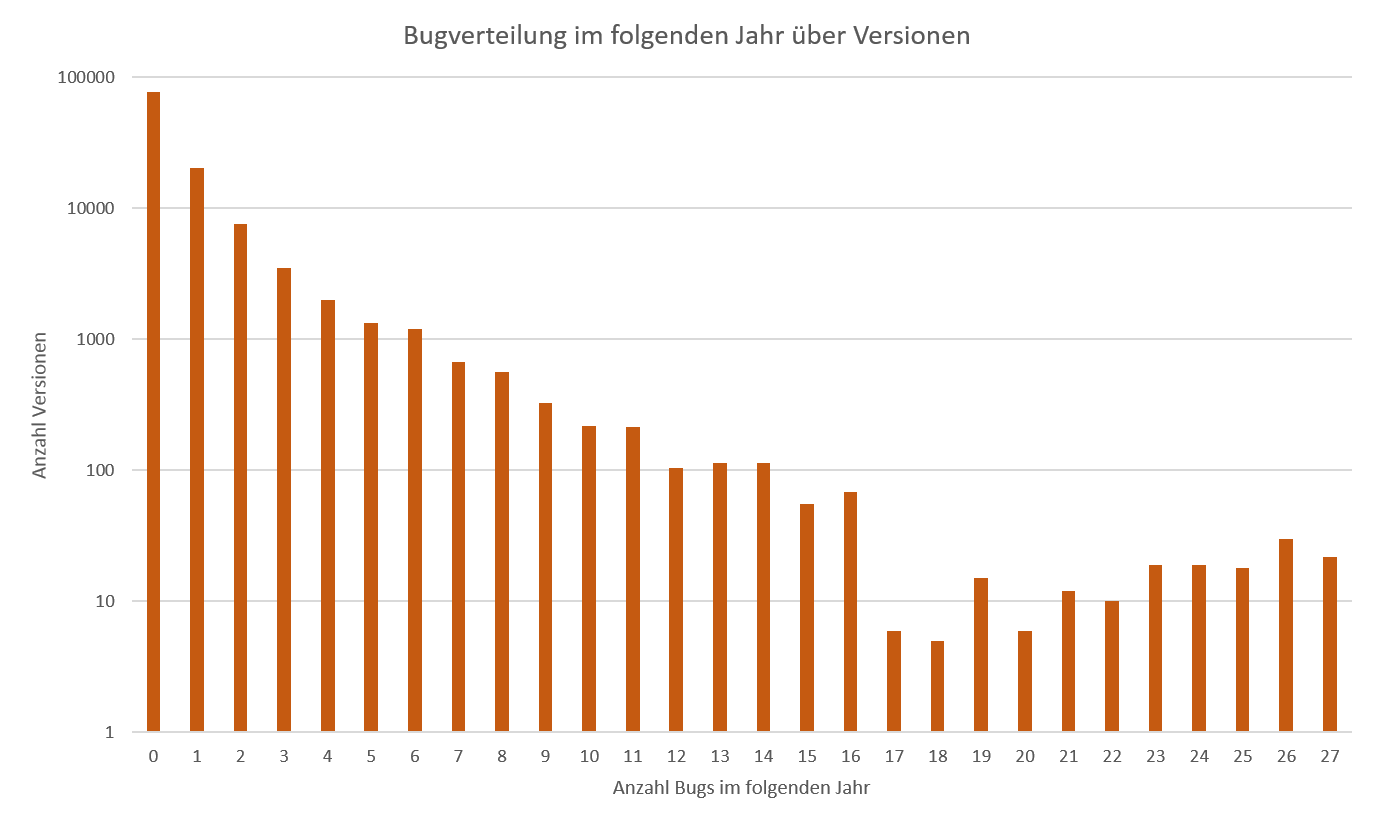
\includegraphics[width=1\textwidth]{resources/images/chart_bug_distribution_1year.png}
	\caption{Anzahl Versionen pro Anzahl Bugs im folgenden Jahr}
	\label{fig:versionbugdist_1year}
\end{figure}

\paragraph{Bugverteilung über Versionen} Die Bugverteilung über die gesamte Lebenszeit von Files ist ein interessantes Mass, welches einiges über die Qualität eines Projekts verrät. Für den Zweck dieser Arbeit viel interessanter ist jedoch die Verteilung von \emph{aufkommenden} Bugs pro \emph{Version}.

So zeigen die Abbildungen \ref{fig:versionbugdist_1month}, \ref{fig:versionbugdist_6month} und \ref{fig:versionbugdist_1year} die Verteilung von kommenden Bugs pro Version für den folgenden Monat resp. die folgenden 6 Monate und das folgende Jahr. Als aufkommende Bugs für eine Version gelten alle zukünftigen Commits in der jeweiligen Zeitspanne, welche auf dasselbe File verweisen und über das Issue-Tracking als Bugfix markiert sind.

Es ist auch hier wichtig zu beachten, dass die Y-Achse dieser drei Grafiken logarithmisch skaliert ist. Es ist auffallend, dass die Verteilung so annähernd linear wird, was auf eine Poisson-Verteilung hindeutet. Die Ungenauigkeiten könnten einfach von Ausreissern stammen, es wäre aber möglich, dass der Grund dafür eine Nicht-Unabhängigkeit der Ereignisse ist. Wir vermuten, dass ein Bugfix die Wahrscheinlichkeit für weitere Bugfixes wesentlich beeinflusst, was der Grund für das Implementieren der temporalen Features war (siehe Kapitel \ref{sec:temporalfeatures}). Die Beobachtung dieser annähernden Poisson-Verteilung führte zur Idee, einen Log-Transform auf dem Target-Vektor auszuführen. Dies wird im Kapitel \ref{sec:log_transform_results} genauer beschrieben.

Ein weiterer interessanter Punkt ist, dass sich die Verteilung über die verschiedenen Zeitspannen nicht massgeblich unterscheidet. Erwartungsgemäss gibt es bei grösseren Zeitspannen aber mehr Ausreisser die eine sehr hohe Buganzahl aufweisen.

\begin{figure}[!ht]
	\centering
	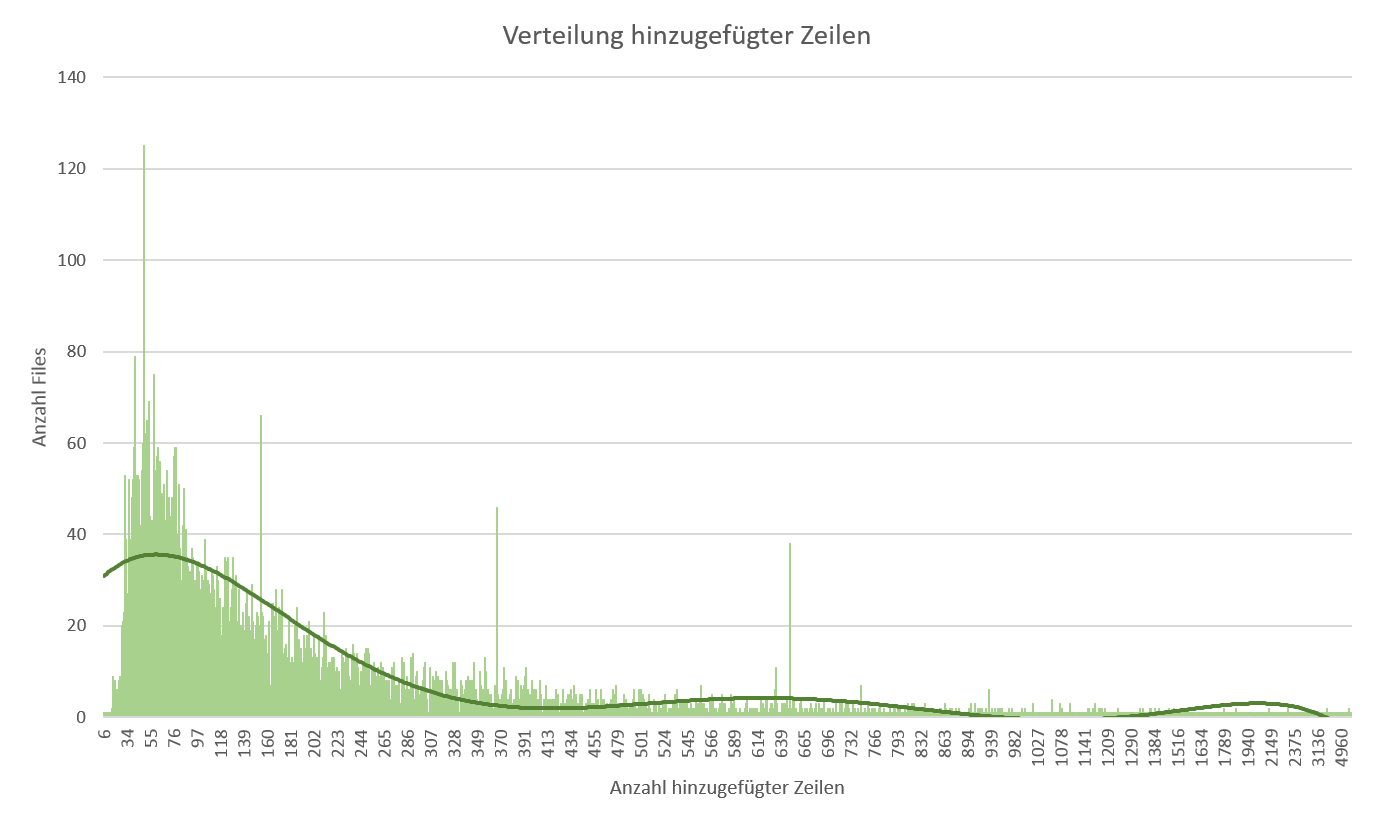
\includegraphics[width=1\textwidth]{resources/images/chart_addition_distribution.png}
	\caption{Anzahl Files pro Anzahl hinzugefügter Zeilen}
	\label{fig:filecountperadditions}
\end{figure}

\begin{figure}[!ht]
	\centering
	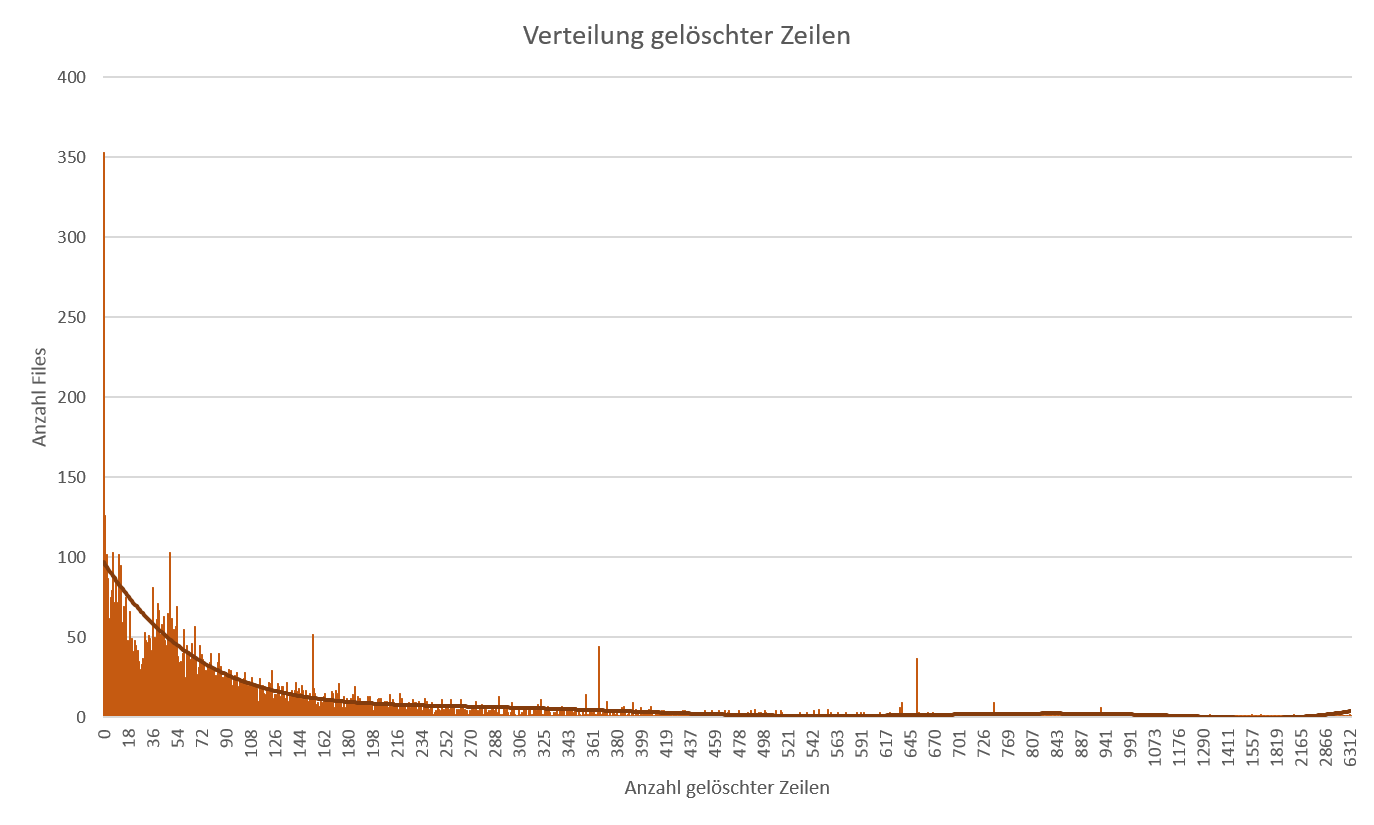
\includegraphics[width=1\textwidth]{resources/images/chart_deletion_distribution.png}
	\caption{Anzahl Files pro Anzahl gelöschter Zeilen}
	\label{fig:filecountperdeletions}
\end{figure}

\paragraph{Verteilung von Changes} Mit den Abbildungen \ref{fig:filecountperadditions} und \ref{fig:filecountperdeletions} wird die Verteilung von Zeilenänderungen dargestellt. Die Grafiken zeigen, dass bei den meisten Files über ihre gesamte Lebensdauer zwischen 30 und 100 Zeilen hinzugefügt werden. Das impliziert auch, dass die meisten Files nicht grösser als 100 Zeilen sind. Die Verteilung der gelöschten Zeilen zeigen, dass bei vielen Files nur wenig gelöscht wird. An dieser Stelle sei nochmals darauf hingewiesen, dass auch eine Zeilenänderung als gelöschte Zeile gilt.

% Ist Filesize Verteilung interessant? -> Nein glaube nicht

\subsubsection{Stichproben von Java Files} \label{sec:filesamplestatistics}

Im Folgenden werden einige ausgewählte Java-Dateien des Projekts \emph{Elasticsearch} genauer analysiert.

Die ``Issues über Zeit''-Statistiken zeigen,  wie die verschiedenen Issues über die Zeitachse der Datei-Lebenszeit verteilt sind.

\paragraph{InternalEngine.java} Diese Java-Klasse wurde ausgewählt, weil sie die höchs\-te Bug-Anzahl (53) aufweist. Da diese Datei eine Kernkomponente ist, welche seit dem Initial-Commit im Projekt vorhanden ist, bestehen vermutlich auch viele Abhängigkeiten, was dazu führte, dass sie mit eben so vielen Bugs in Verbindung gebracht wird. Gerade deswegen bietet sie aber die beste Grundlage für eine genauere Analyse.

\begin{figure}[!ht]
	\centering
	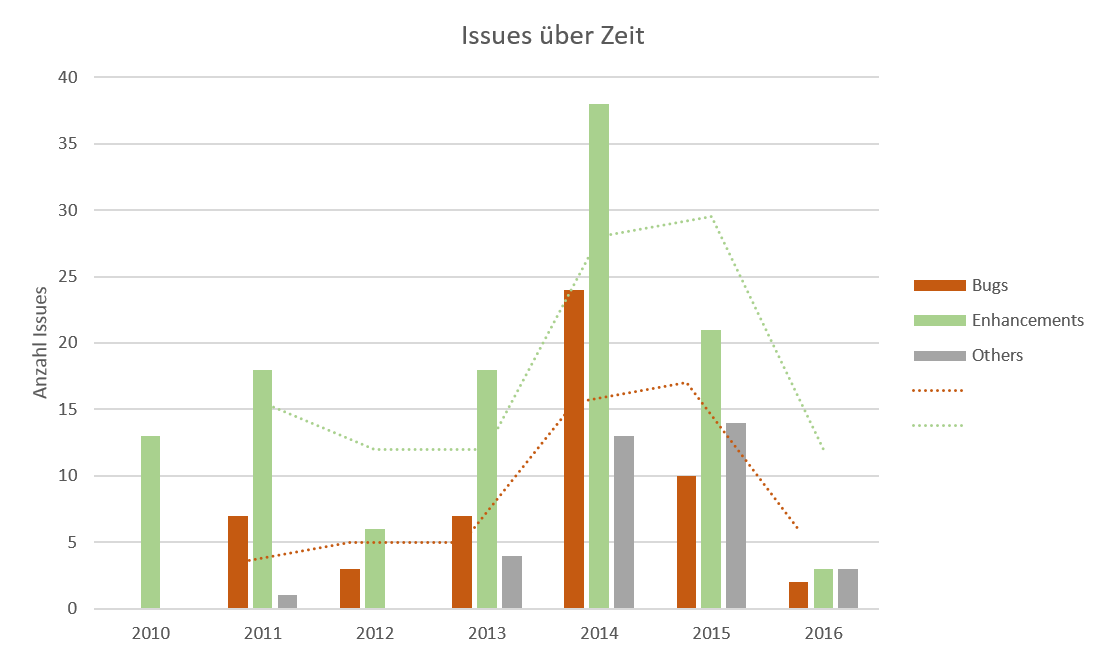
\includegraphics[width=1\textwidth]{resources/images/issues_over_time_internalengine.png}
	\caption{Anzahl Enhancements und Bugs, welche auf InternalEngine.java referenzieren, über die Zeit}
	\label{fig:issues_over_time_internalengine}
\end{figure}

Stellt man die Anzahl Issues, gruppiert nach ihrem Typ (Enhancement und Bug), auf einer Zeitachse dar (siehe Abbildung \ref{fig:issues_over_time_internalengine}), lässt sich feststellen, dass die Anzahl Bugs pro Jahr proportional zur Anzahl Enhancements im selben Jahr ist. Dies bestätigt die Vermutung, das Enhancements neue Programmfeatures hinzufügen, in welchen Bugs vorhanden sind.

\begin{figure}[!ht]
	\centering
	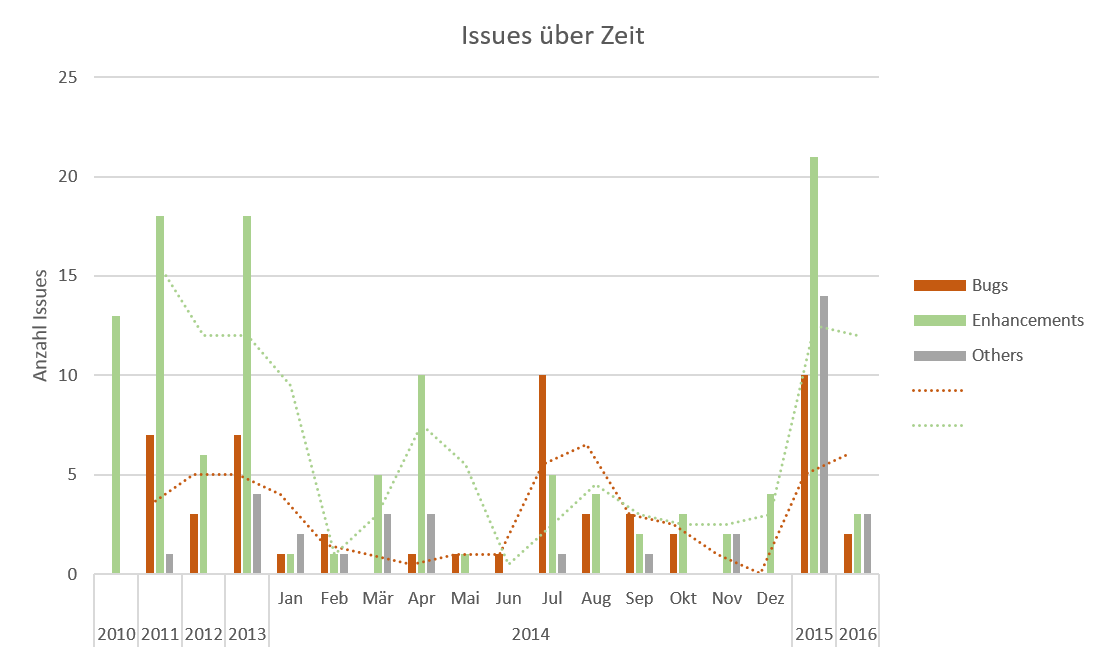
\includegraphics[width=1\textwidth]{resources/images/issues_over_time_internalengine2.png}
	\caption{Anzahl Enhancements und Bugs, welche auf InternalEngine.java referenzieren, über die Zeit, Fokus auf 2014}
	\label{fig:issues_over_time_internalengine2}
\end{figure}

Sieht man sich die Verteilung in einem Jahr genauer an (in Abbildung \ref{fig:issues_over_time_internalengine2} das Jahr 2014) lässt sich das sogar noch besser aufzeigen. Auf eine grosse Anzahl von Enhancements folgt, um ca. 3 Monate versetzt, eine ebenso grosse Anzahl von Bugs. Dasselbe Phänomen kann auch in anderen Jahren beobachtet werden. Auf jede ``Welle'' von Enhancements folgt kurze Zeit später eine ähnliche ``Welle'' von Bugs.

\paragraph{ChildQuerySearchIT.java} Dieses File weist mit 31 Bugs ebenfalls eine sehr hohe Anzahl von Bugs auf und ist deshalb für eine Analyse gut geeignet.

\begin{figure}[!ht]
	\centering
	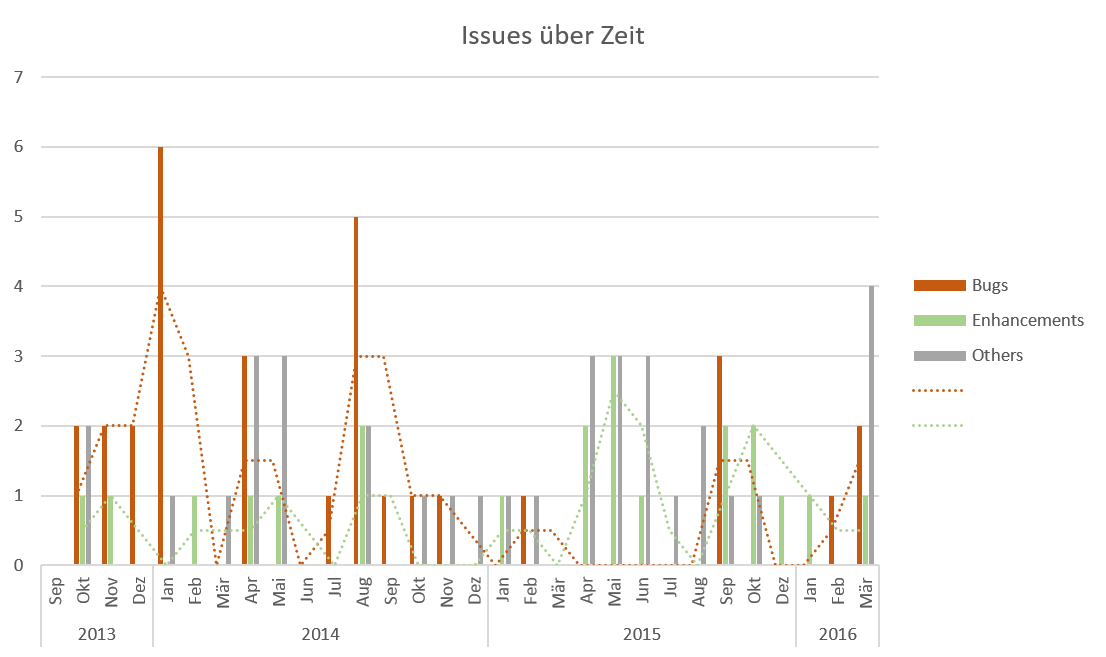
\includegraphics[width=1\textwidth]{resources/images/issues_over_time_childquerysearch.png}
	\caption{Anzahl Enhancements und Bugs, welche auf ChildQuerySearchIT.java referenzieren, über die Zeit}
	\label{fig:issues_over_time_childquerysearch}
\end{figure}

In der Abbildung \ref{fig:issues_over_time_childquerysearch} sind die zwei Spitzen der Bug-Anzahl Ende 2013 und Mitte 2014 auffällig. Ausserdem ist hier gut ersichtlich, dass ein Source File tendenziell am Anfang seiner Lebenszeit mehr Bugs aufweist, was darauf zurückzuführen ist, dass dann auch am meisten neuer Code geschrieben wird. Hier sind die meisten Bugs, inklusive den beiden Ausreissern im ersten Drittel der Lebenszeit des Files zu verzeichnen. Danach pendelt es sich ein und zeigt das bereits erwähnte Muster von Enhancement-Wellen mit kurz darauffolgenden Wellen von Bugs.

\subsection{Machine Learning} \label{sec:ml_results}
% Beispiel wie man da machen könnte:
%% Für jeden Lauf:
%%% Verwendetes Modell inkl. Kernel
%%% Mit oder ohne Ngrams
%%% Die 4 Metriken auf Training und Testset
%%% Vergleich mit mind. 1 Metrik (R2 und MAE?) der Baseline
%%% Laufzeit Trainieren
%%% Evtl. Laufzeit Predicten
%% Vermutlich wird das zu viel für eine Tabelle, deshalb sinnvoll aufteilen in mehrere
%% Vom Besten Lauf: Lern- und Validationskurve rein (falls sie sinnvoll aussieht...)
%% Prosa zur Interpretation der Daten

In diesem Kapitel werden die Resultate der im Kapitel \ref{sec:approach_ml} beschriebenen Experimente aufgeführt und besprochen. Als erstes wurden verschiedene \ac{ML}-Modelle miteinander und gegenüber einer Baseline verglichen, anschliessend wurde die Signifikanz der verschiedenen Feature-Gruppen zu bestimmen versucht.

Als Metriken zur Bewertung der \ac{ML}-Modelle wurden der \acf{MAE}, \acf{MDE} und der \(R^2\)-Score verwendet. Für die Bedeutung dieser Werte verweisen wir auf das Kapitel \ref{sec:regressionmetrics}, wo sie kurz beschrieben werden.

Aufgrund von zeitlichen Einschränkungen wurden alle der folgenden Experimente auf nur einer Trainings- und Testset Kombination durchgeführt (siehe Tabelle \ref{tab:testdata_for_results}). Dies schränkt die Aussagekraft der erhaltenen Resultate natürlich ein. Bei einer weiterführenden Arbeit müsste noch mit vielen anderen Daten getestet werden. Vorschläge, wie man diese Aufgabe angehen könnte, besprechen wir im Kapitel \ref{sec:outlook_experiments}.

\begin{table}[ht]
	\begin{tabular}[c]{rl}
		\hline
		Projekt:		&	\emph{Elasticsearch} \\
		Target:			&	Bugs in den folgenden 6 Monaten \\
		Trainingsset: 	&	01.10.2014 - 31.12.2014 (620 Commits mit 3414 Dateiversionen) \\
		Testset:		&	01.01.2015 - 31.01.2015 (165 Commits mit 950 Dateiversionen) \\
		\hline
	\end{tabular}
	\centering
	\caption{Verwendete Testdaten für Resultate}
	\label{tab:testdata_for_results}
\end{table}

\subsubsection{Baseline} \label{sec:ml_results_baseline}
Um die Performance der erstellten  \ac{ML}-Modelle überprüfen zu können, wurden deren Resultate mit drei verschiedenen Baseline-Predictions verglichen. Die Implementation dieser Baselines wurde im Kapitel \ref{sec:ml_pipeline_implementation} beschrieben.

Zu beachten ist, dass sich diese Baselines auf die Ergebnisse des Testsets beziehen, da mit diesem die Qualität eines \ac{ML}-Modells gemessen wird. Das heisst, dass der Mean, der Median und die Target-Gewichte über die Ground Truth des Trainingsset berechnet wurden. Dann wurde die Vorhersage dieser Baseline-Modelle mit der Ground Truth des Testsets verglichen und daraus die Metriken in Tabelle \ref{tab:baseline_results} berechnet.

% -> Baseline <-
% Baseline wird auf dem *TEST*-Set generiert
% Random kann variieren
\begin{table}[ht]
	\begin{tabular}[c]{|r|l|l|l|}
		\hline
		\textbf{Baseline} & \textbf{MAE} & \textbf{MDE}	& \(\mathbf{R^2}\)\\ \hline
		Mean			& 1.4145	& 0.9060	& -0.0131 \\ \hline
		Median			& 1.1895	& 0.0000	& -0.2314 \\ \hline
		Weighted Random	& 1.6411	& 1.0000	& -0.6142 \\ \hline
	\end{tabular}
	\centering
	\caption{Ergebnisse der Baselines}
	\label{tab:baseline_results}
\end{table}

Keine der Baselines erzielt ein besonders gutes Ergebnis. So sind alle \(R^2\)-Scores negativ. Das heisst, sie bilden die Varianz der Ground Truth sehr schlecht ab, was aber gerade bei den statischen Modellen Mean und Median zu erwarten war. Wir hätten ein besseres Resultat der Weighted Random Baseline erwartet, da sie eigentlich mehr Informationen in ihr Modell einfliessen lässt. Auffallend ist weiterhin, dass die Median-Baseline einen \ac{MDE} von 0 hat. Der Grund dafür ist, dass der Median des Target-Vektors der Ground Truth in der Regel auch 0 ist, da die meisten Dateiversionen keinen Bug in den folgenden 6 Monaten erwarten. Somit ist die Vorhersage der Median-Baseline für die meisten Datensätze korrekt. Der \ac{MAE} ist aber trotzdem eher hoch.
Zuletzt ist noch anzumerken, dass die Weighted Random Baseline naturgemäss variiert. Dies allerdings nicht so stark, dass es für die Anwendung als Baseline signifikant wäre.

\subsubsection{Vergleich der ML-Modelle} \label{sec:ml_results_models}
In einer ersten Phase der Experimente wurden verschiedene Konfigurationen der möglichen \ac{ML}-Modelle getestet und miteinander verglichen.

\paragraph{Resultate ohne N-Grams}
Die Tabelle \ref{tab:results_without_ngrams} zeigt die erhaltenen Resultate, welche \emph{ohne} die Einbeziehung von N-Grams gewonnen wurden.

Erwartungsgemäss hat lineare Regression mit Abstand am schlechtesten abgeschnitten. Es gelingt zwar, das Modell den Trainingsdaten anzupassen, das Modell generalisiert aber sehr schlecht. Wieso die Ergebnisse auf dem Testset dermassen schlecht sind, ist uns nicht ganz klar. Wir vermuten, dass das Modell aufgrund linear voneinander abhängigen Features stark verzerrt ist und deshalb auf unbekannten Daten unsinnige Ergebnisse produziert.

Ridge Regression wurde in zwei Konfigurationen getestet. Einmal ohne polynomiale Features (Ridge Regression PD1) und einmal mit polynomialen Features 2. Grades (Ridge Regression PD2). Bereits ohne polynomiale Features zeigt sich, dass die Regularisierung die Resultate auf dem Testset gegenüber Linearer Regression massiv zu verbessern vermag. Polynomiale Features 2. Grades verbessern die Performance von Ridge Regression noch mehr und können bereits brauchbare Resultate liefern. Ein Nachteil ist hier der hohe Speicherbedarf. Es wurde versucht, polynomiale Features 3. Grades einzusetzen, dies führte aber bereits zu einem Speicherbedarf von über 40 GB, womit unsere Infrastruktur überfordert war. Es ist anzunehmen, dass sich bei grösseren Trainingssets auch schon der 2. Grad als zu speicherhungrig herausstellt.

SVR benötigt zwar nicht so viel Speicher, dafür aber bedeutend mehr Rechenzeit. SVR linear, also ohne Kernelfunktion, schneidet bedeutend besser ab als lineare Regression. Grund dafür ist wie bei Ridge Regression mehrheitlich die eingesetzte Regularisierung. Die Performance von SVR polynomial liegt etwas unter Ridge Regression mit polynomialen Features 2. Grades. Dafür war hier auch der Einsatz von Grad 3 möglich, ohne dass dies zu einem Memory Error geführt hat. Die besten Resultate erzielte eindeutig SVR mit \ac{RBF}-Kernel. Dieses Modell führte sowohl auf dem Trainings- als auch auf dem Testset zu akzeptablen Ergebnissen mit einem sehr hohen Bestimmtheitsmass und einem mittleren Fehler \(<1\). Der Sigmoid-Kernel konnte hingegen nicht überzeugen und produzierte das zweitschlechteste Resultat nach Linearer Regression.

% -> Ohne N-Grams <-
% Ridge Reg mit PD3 -> Memory Error
\begin{table}[ht]
	\begin{tabular}[c]{|r|r|l|l|l|}
		\hline
		\textbf{Modelltyp} & \textbf{Set} & \textbf{MAE} & \textbf{MDE}	& \(\mathbf{R^2}\) \\ \hline
		\multirow{2}{*}{Lineare Regression}
		& Training 	& 0.7929 & 0.5200 & 0.5937 \\ \cline{2-5}
		& Test 		& \(4.035 \cdot 10^9\) & 5.9635 & \(-1.744 \cdot 10^{20}\) \\ \hline
		\multirow{2}{*}{Ridge Regression PD1}
		& Training 	& 0.7858 & 0.4980 & 0.5600 \\ \cline{2-5}
		& Test 		& 1.1120 & 0.6866 & 0.3960 \\ \hline
		\multirow{2}{*}{Ridge Regression PD2}
		& Training 	& 0.3702 & 0.2127 & 0.8914 \\ \cline{2-5}
		& Test 		& 1.0142 & 0.6385 & 0.6103 \\ \hline
		\multirow{2}{*}{SVR Linear}
		& Training 	& 0.3126 & 0.1000 & 0.8387 \\ \cline{2-5}
		& Test 		& 0.9532 & 0.5141 & 0.5284 \\ \hline
		\multirow{2}{*}{SVR Polynomial}
		& Training 	& 0.4267 & 0.1000 & 0.7170 \\ \cline{2-5}
		& Test 		& 0.8795 & 0.3658 & 0.5639 \\ \hline
		\multirow{2}{*}{SVR RBF}
		& Training 	& 0.3084 & 0.1001 & 0.8439 \\ \cline{2-5}
		& Test 		& 0.8343 & 0.4732 & 0.7004 \\ \hline
		\multirow{2}{*}{SVR Sigmoid}
		& Training 	& 0.7174 & 0.2351 & 0.3861 \\ \cline{2-5}
		& Test 		& 0.9669 & 0.2951 & 0.2697 \\ \hline
	\end{tabular}
	\centering
	\caption{Performance der verschiedenen \ac{ML}-Modelle \emph{ohne} Einsatz von N-Grams}
	\label{tab:results_without_ngrams}
\end{table}

\paragraph{Resultate mit N-Grams} 
Nachdem mit den herkömmlichen Features getestet wurde, wurden zusätzlich noch N-Grams aktiviert. Das erfordete den Einsatz von Sparse-Matrizen, ansonsten wurde die Konfiguration der jeweiligen Modelle identisch belassen. Die Resultate dieser Durchläufe sind in Tabelle \ref{tab:results_with_ngrams} zusammengestellt.

Lineare Regression führte auch hier zu äussert schlechten Ergebnissen. Im Unterschied zu den Experimenten ohne N-Grams reichte hier die Regularisierung von Ridge Regression (PD1) aber scheinbar nicht, um das Resultat zu verbessern. Da sich das Modell aber scheinbar sehr gut auf das Trainingsset angepasst hat, ist hier von sehr starkem Overfitting auszugehen. Bei einem weiteren Versuch müsste man versuchen, den Regularisierungsparameter \(C\) noch weiter zu verringern.

Das Erzeugen von polynomialen Features (für Ridge Regression PD2) war mit N-Grams nicht möglich, da dies aus der Sparse-Matrix eine Dense-Matrix erzeugt hätte. Wenn dann daraus noch Polynome erstellt würden, stiege der Speicherbedarf enorm.

Wie auch bei Ridge Regression vermochte die Regularisierung von SVR Linear hier nicht, das Resultat auf dem Testset im Gegensatz zu Linearer Regression signifikant zu verbessern. Wir erhofften uns, dass SVR Polynomial sinnvolle Resultate erzeugen würde, da wie bereits erwähnt polynomiale Features mit N-Grams nicht möglich waren. Leider wies dieses Modell eine enorm lange Laufzeit auf, so dass es nach über 27 Stunden terminiert werden musste, ohne dass es Resultate produziert hatte.

Genau wie bei den Experimenten ohne N-Grams erwies sich auch hier der \ac{RBF}-Kernel als der Effektivste. Er terminierte nicht nur in sinnvoller Zeit, sondern produzierte auch ein sinnvolles Ergebnis. Der Sigmoid-Kernel erwies sich abermals als nicht nützlich für diesen Anwendungsfall.

Leider können diese Resultate nur beschränkt einen positiven Nutzen von N-Grams zeigen. Einzig der \ac{MDE} erfährt eine Verbesserung. Der \(R^2\)-Score ist auf dem Testset deutlich schlechter als beim selben Experiment ohne N-Grams. Hingegen ist der \(R^2\)-Score auf dem Trainingsset sehr hoch. Dies deutet eigentlich auf Overfitting hin, die Validationskurve (siehe Abbildung \ref{fig:svr_rbf_validation_curves}) spricht da aber eher dagegen. Die Lernkurve (siehe Abbildung \ref{fig:svr_rbf_learning_curves}) unterstützt die Vermutung, dass für N-Grams schlicht mehr Trainingsdaten benötigt werden. Ebenfalls anzumerken ist, dass aufgrund der langen Laufzeiten bei diesen Experimenten auf das Einbeziehen von weiteren Parametern wie \emph{gamma} und \emph{epsilon} in die Cross Validation verzichtet wurde. Mit dem Finden von besseren Parametern könnte das Ergebnis vermutlich verbessert werden.
% die hohen r2 werte
% mehr cv machen 

% -> Mit N-Grams <-
% keine polynomial features weil das riesig würde und dense -> memory
% kein svr poly weil auch noch über 12 stunden nicht terminiert -> kA wieso
% Evtl. schlechtere ergebnisse da weniger CV aus Zeitgrpnden
\begin{table}[ht]
	\begin{tabular}[c]{|r|r|l|l|l|}
		\hline
		\textbf{Modelltyp} & \textbf{Set} & \textbf{MAE} & \textbf{MDE}	& \(\mathbf{R^2}\) \\ \hline
		\multirow{2}{*}{Lineare Regression}
		& Training 	& 0.0722 & 0.0354 & 0.9939 \\ \cline{2-5}
		& Test 		& \(5.112 \cdot 10^{10}\) & \(1.185 \cdot 10^{10}\) & \(-2.088 \cdot 10^{21}\) \\ \hline
		\multirow{2}{*}{Ridge Regression PD1}
		& Training 	& 0.1148 & 0.0422 & 0.9838 \\ \cline{2-5}
		& Test 		& 1134.684 & 0.5785 & \(-9.413 \cdot 10^7\) \\ \hline
		\multirow{2}{*}{Ridge Regression PD2}
		& Training 	& N/A & N/A & N/A \\ \cline{2-5}
		& Test 		& N/A & N/A & N/A \\ \hline
		\multirow{2}{*}{SVR Linear}
		& Training 	& 0.1310 & 0.1000 & 0.9749 \\ \cline{2-5}
		& Test 		& 916.5596 & 0.5371 & \(5.387 \cdot 10^7\) \\ \hline
		\multirow{2}{*}{SVR Polynomial}
		& Training 	& N/A & N/A & N/A \\ \cline{2-5}
		& Test 		& N/A & N/A & N/A \\ \hline
		\multirow{2}{*}{SVR RBF}
		& Training 	& 0.1320 & 0.0999 & 0.9774 \\ \cline{2-5}
		& Test 		& 0.8688 & 0.3723 & 0.4794 \\ \hline
		\multirow{2}{*}{SVR Sigmoid}
		& Training 	& 0.9404 & 0.1000 & -0.1846 \\ \cline{2-5}
		& Test 		& 1.2143 & 0.1000 & -0.1942 \\ \hline
	\end{tabular}
	\centering
	\caption{Performance der verschiedenen \ac{ML}-Modelle \emph{mit} Einsatz von N-Grams}
	\label{tab:results_with_ngrams}
\end{table}

\paragraph{Laufzeiten}
Um die Modelle zu vergleichen, wurden auch die Laufzeiten für das Trainieren, resp. das Predicten erfasst. Denn für einen sinnvollen Einsatz einer Fehlervorhersage muss auch gewährleistet sein, dass die Lösung in nützlicher Zeit terminiert und Vorhersagen machen kann.

% Laufzeit ohne NGrams
\begin{table}[ht]
	\begin{tabular}[c]{|r|l|l|}
		\hline
		\textbf{Modelltyp}		& \textbf{Training}	& \textbf{Prediction}	\\ \hline
		Lineare Regression		& 1 s				& \textless 1 s			\\ \hline
		Ridge Regression PD1 	& 5 s				& \textless 1 s			\\ \hline
		Ridge Regression PD2	& 3 s				& \textless 1 s			\\ \hline
		SVR Linear				& 1 h 3 min 25 s 	& 2 min 3 s				\\ \hline
		SVR Polynomial			& 54 s				& 4 s					\\ \hline
		SVR RBF					& 2 min 30 s		& 3 s					\\ \hline
		SVR Sigmoid				& 2 min 40 s		& 3 s					\\ \hline
	\end{tabular}
	\centering
	\caption{Laufzeit der verschiedenen \ac{ML}-Modelle \emph{ohne} Einsatz von N-Grams}
	\label{tab:runtime_without_ngrams}
\end{table}

Die Tabelle \ref{tab:runtime_without_ngrams} zeigt die Laufzeit der verschiedenen \ac{ML}-Konfigurationen der ersten Experimentserie ohne N-Grams. Lineare Regression und Ridge Regression sind erwartungsgemäss sehr schnell. Mit SVR performt der polynomial-Kernel am Besten, \ac{RBF} und Sigmoid benötigen vergleichsweise eher lange. Überraschend ist hier die unverhältnismässig lange Laufzeit von SVR Linear. Da hier keine Kernel-Funktion eingesetzt wird, wäre eigentlich eine kürzere Laufzeit als bei den restlichen SVR-Konfigurationen zu erwarten gewesen. Wir haben keine gute Erklärung für dieses Verhalten. Es ist nicht auszuschliessen, dass es sich hierbei um eine Eigenheit der Implementation von \emph{scikit-learn} handelt.

% Laufzeit mit NGrams
\begin{table}[ht]
	\begin{tabular}[c]{|r|l|l|}
		\hline
		\textbf{Modelltyp}		& \textbf{Training}	& \textbf{Prediction}	\\ \hline
		Lineare Regression		& 54 s				& 2s					\\ \hline
		Ridge Regression PD1 	& 14 min 29 s		& 21 s					\\ \hline
		Ridge Regression PD2	& N/A				& N/A					\\ \hline
		SVR Linear				& 13 h 33 min 3 s	& 12 min 42 s			\\ \hline
		SVR Polynomial			& \textgreater 27 h & N/A					\\ \hline
		SVR \ac{RBF}					& 55 min 8 s		& 13 min 26 s			\\ \hline
		SVR Sigmoid				& 47 min 9 s		& 10 min 35 s			\\ \hline
	\end{tabular}
	\centering
	\caption{Laufzeit der verschiedenen \ac{ML}-Modelle \emph{mit} Einsatz von N-Grams}
	\label{tab:runtime_with_ngrams}
\end{table}

Werden N-Grams miteinbezogen steigt die Laufzeit mit allen \ac{ML}-Modellen signifikant an. Ridge Regression mit polynomialen Features (PD2) konnten wie bereits erklärt aufgrund von Speichermangel nicht eingesetzt werden. Auch hier benötigte SVR Linear äusserst lange. Mit N-Grams hat aber die mit Abstand längste Laufzeit SVR mit einem polynomial-Kernel. Wir mussten den Lernvorgang nach über 27 Stunden abbrechen. Vermutlich liegt das an der viel höheren Zahl an Features, welche mit N-Grams entstehen. SVR mit \ac{RBF}-Kernel hat zwar mit fast einer Stunde auch eher lange, damit lässt sich aber arbeiten. Mit N-Grams wird ausserdem deutlich, dass SVR-Modelle im Vergleich zu Linearer und Ridge Regression deutlich länger für Vorhersagen benötigen.

\paragraph{Details zu SVR mit RBF-Kernel}
Da SVR in Kombination mit einem RBF-Kernel zu den besten Resultaten führte, soll im Folgenden noch etwas detaillierter auf diese Ergebnisse eingegangen werden.

Abbildung \ref{fig:svr_rbf_learning_curves} zeigt die Lernkurve der Durchläufe ohne und mit N-Grams. Sie zeigt den erreichten \(R^2\)-Score des Modells in Bezug auf die Grösse des Trainingssets. Hier fällt auf, dass sowohl der Score auf dem Trainingsset als auch der \ac{CV}-Score fast linear steigt. Dies deutet darauf hin, das mit noch grösseren Datensets bessere Ergebnisse zu erwarten sind.

\begin{figure}[!ht]
	\centering
	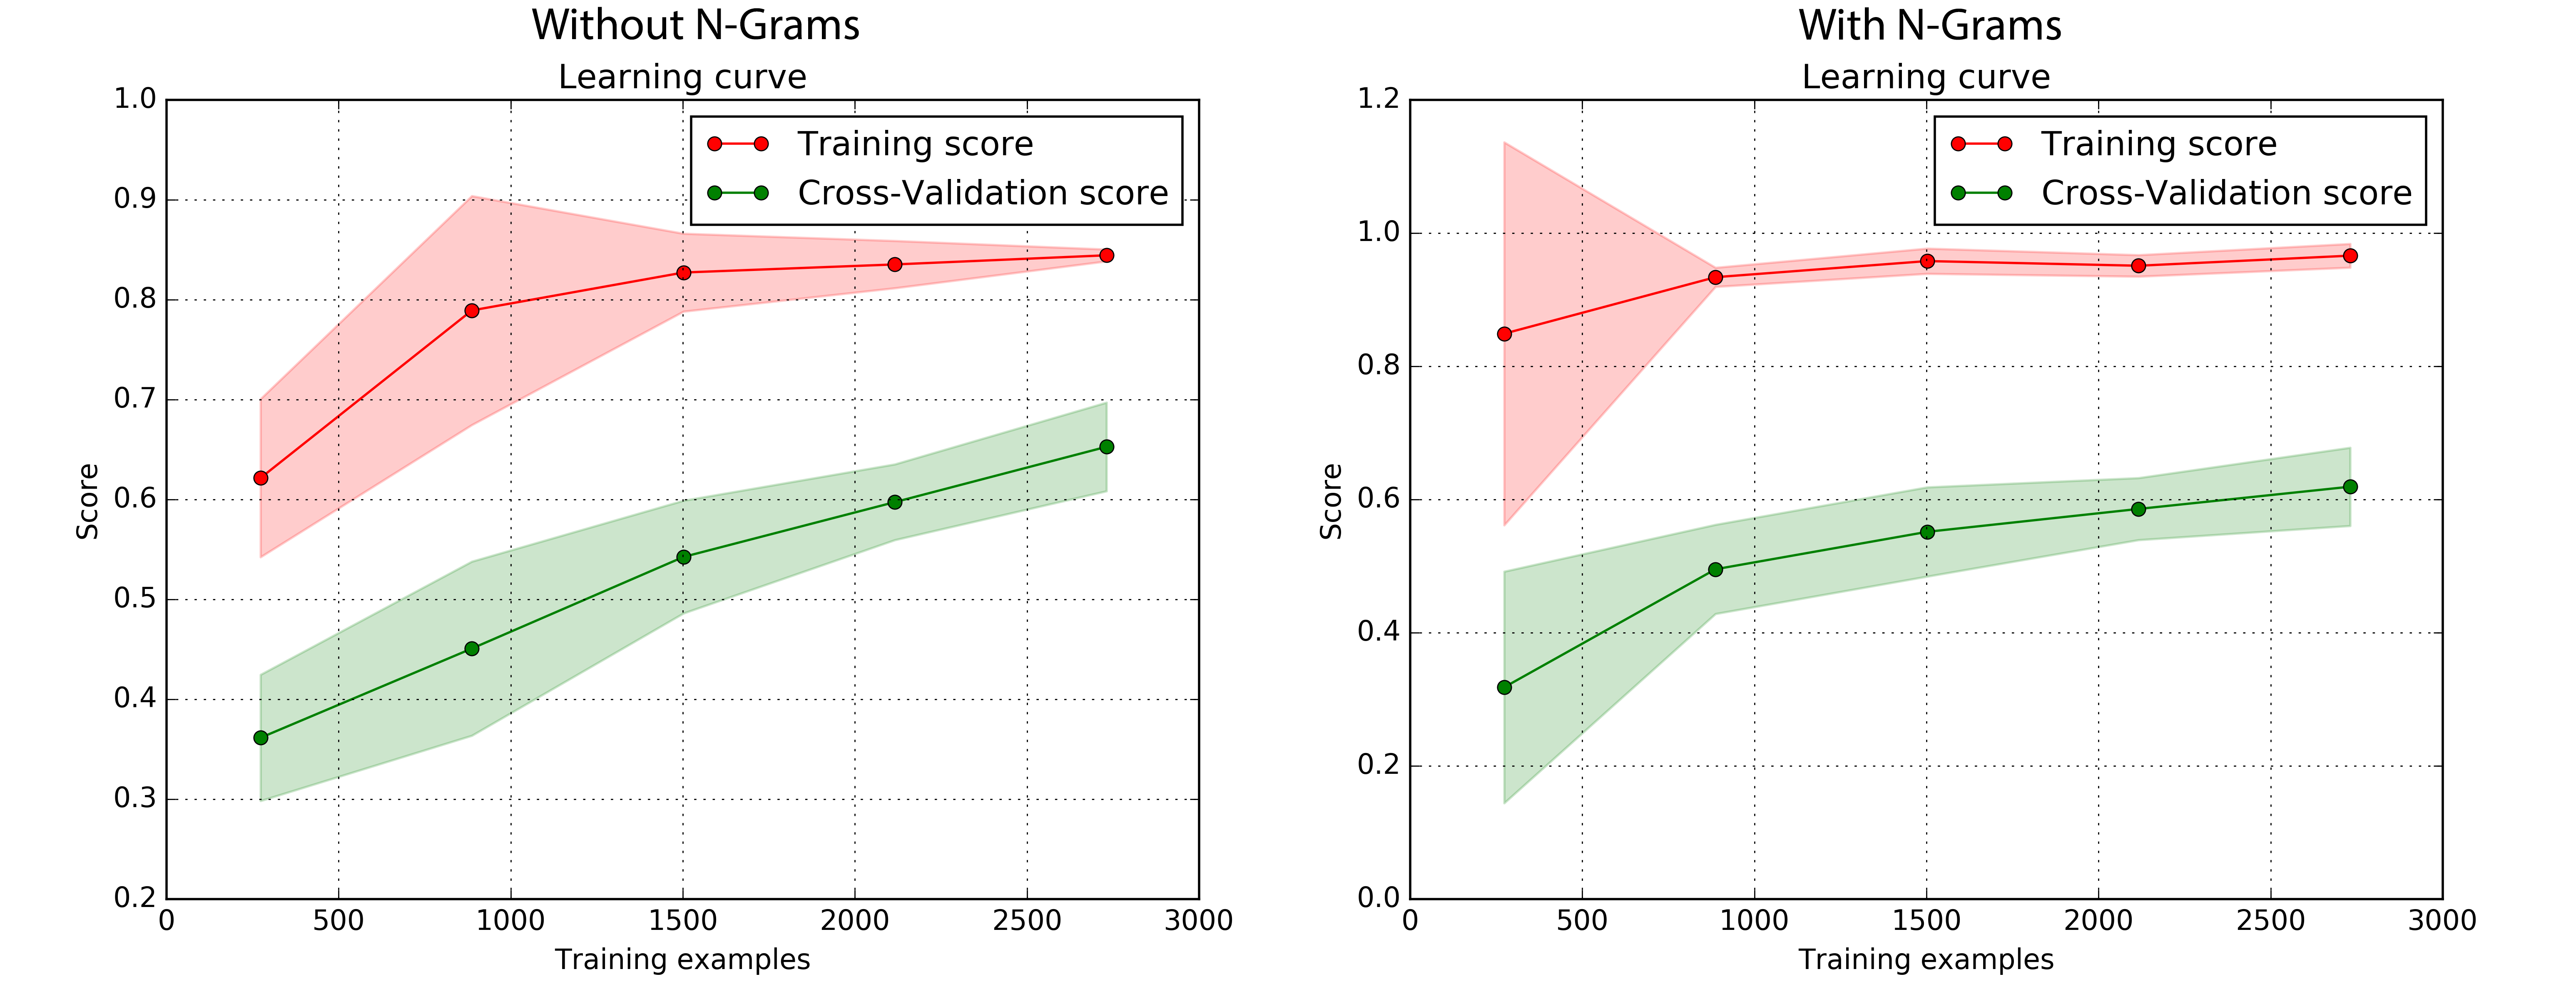
\includegraphics[width=1\textwidth]{resources/images/svr_rbf_learning_curves.png}
	\caption[Lernkurve des SVR-Modells mit RBF-Kernel]{Lernkurve: (\(R^2\))-Score nach Grösse des Trainingssets, SVR-Modell mit RBF-Kernel. Links: ohne N-Grams. Rechts: mit N-Grams}
	\label{fig:svr_rbf_learning_curves}
\end{figure}

Abbildung \ref{fig:svr_rbf_validation_curves} stellt die Validationskurve ohne und mit N-Grams dar. Sie zeigt den erreichten \(R^2\)-Score des Modells in Bezug auf den Regularisierungsparameter \(C\). Beide Kurven erreichen den optimalen Parameter zwischen 1 und 50. Sie flachen sowohl links als auch rechts ab, was darauf hindeutet, dass eine breitere Auswahl an Parametern keinen grossen Nutzen hätte. Auffallend ist ausserdem, dass ohne N-Grams bei grösseren \(C\)s Overfitting auftritt. Dieses kann alleine durch Regularisierung scheinbar nicht verhindert werden, da bei kleineren \(C\)s sowohl der Test- als auch der \ac{CV}-Score schlechter wird.

\begin{figure}[!ht]
	\centering
	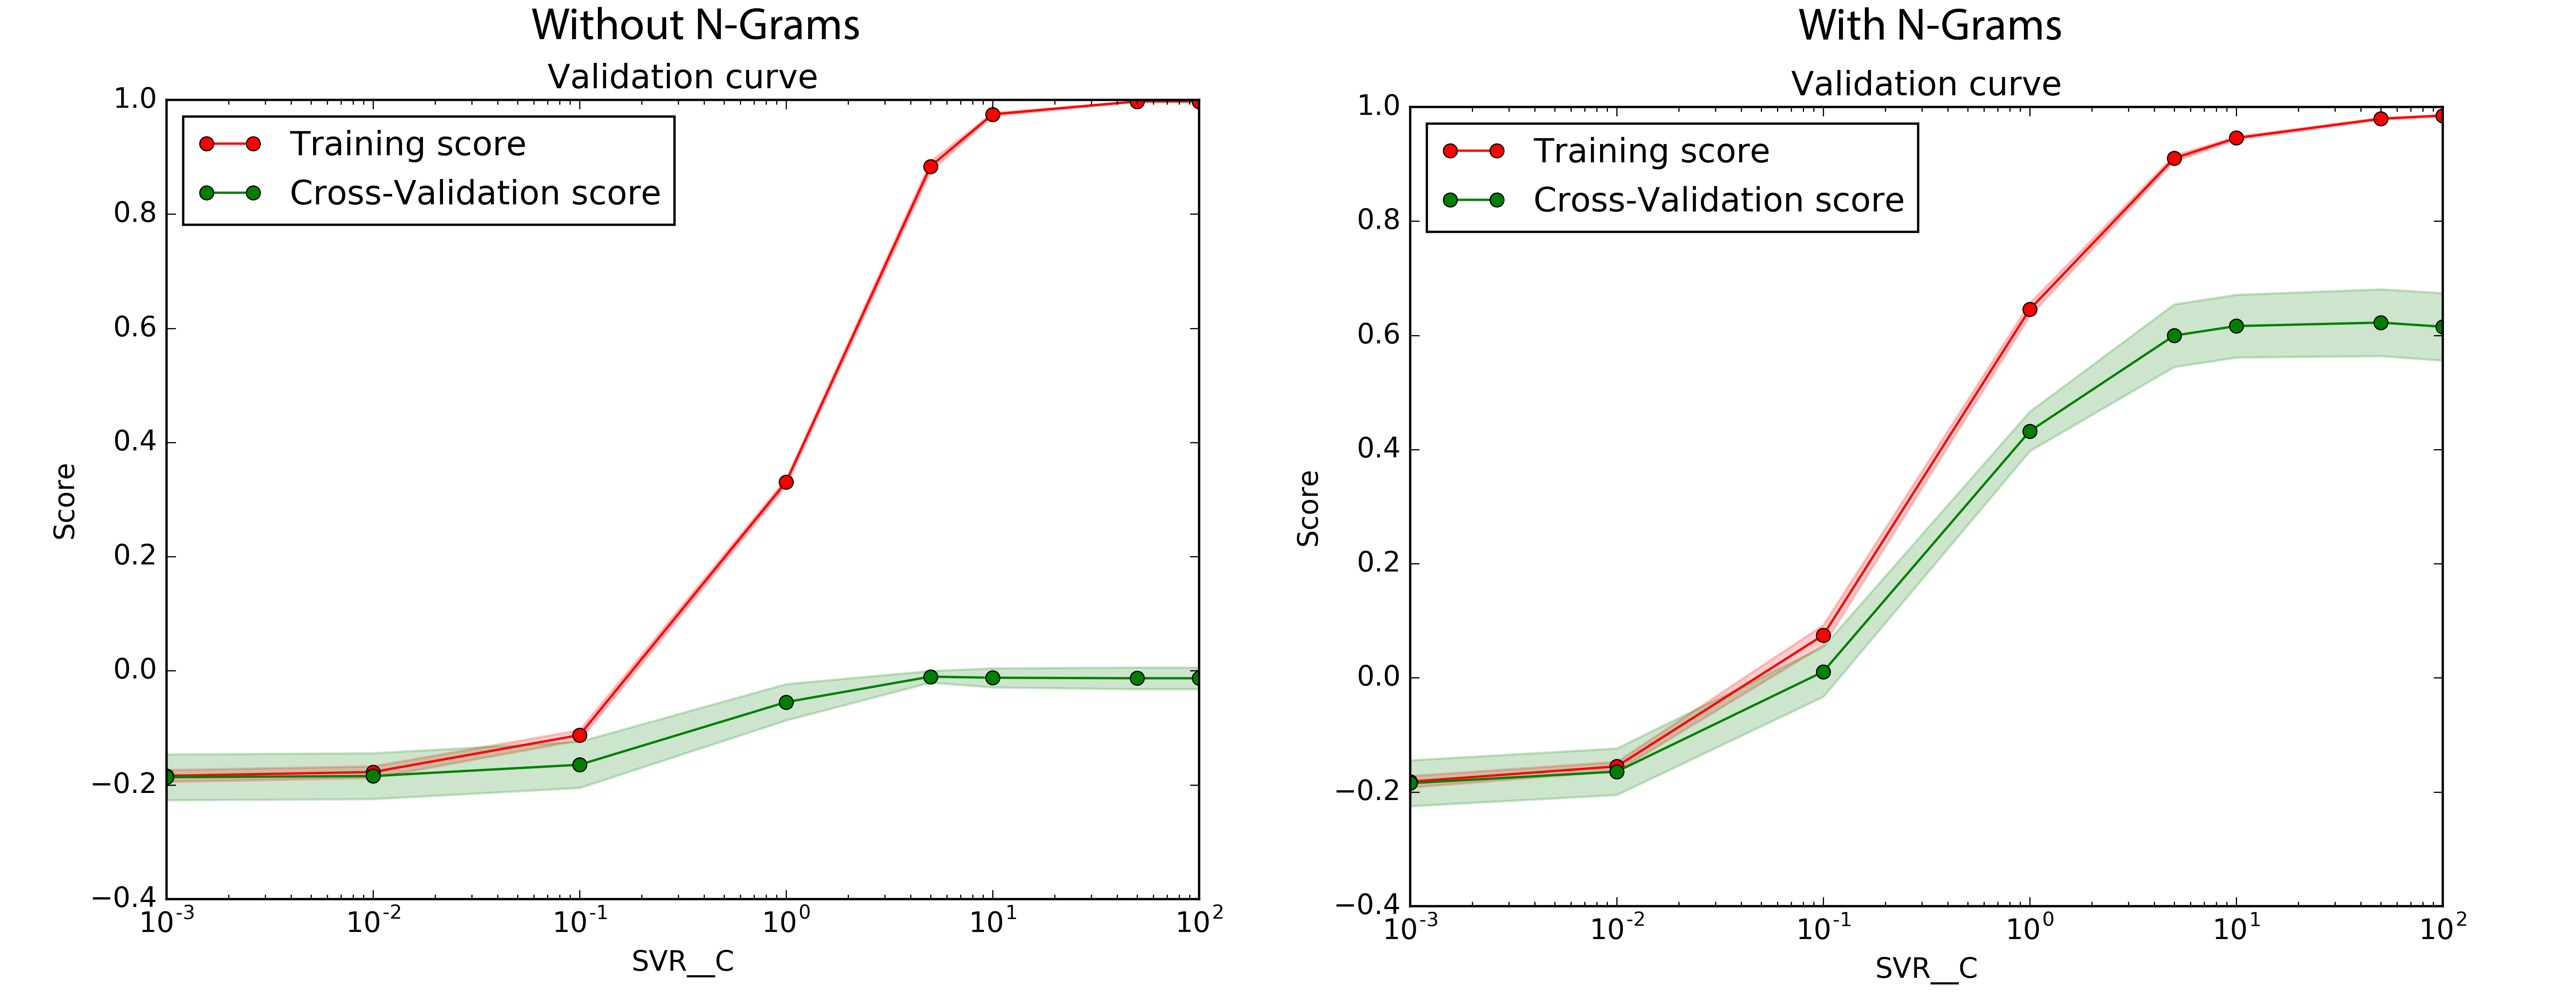
\includegraphics[width=1\textwidth]{resources/images/svr_rbf_validation_curves.png}
	\caption[Validationskurven des SVR-Modells mit RBF-Kernel]{Validationskurve: (\(R^2\))-Score nach \(C\)-Parameter des \newline SVR-Modells mit RBF-Kernel. Links: ohne N-Grams. Rechts: mit N-Grams}
	\label{fig:svr_rbf_validation_curves}
\end{figure}

Die beiden Tabellen \ref{tab:confusion_matrix_without_ngrams} und \ref{tab:confusion_matrix_with_ngrams} zeigen die Confusion-Matrix für die Test-Prediction ohne resp. mit N-Grams. Daran lässt sich die Verteilung der Vorhersagen ablesen. Um dies zu ermöglichen, wurden die vorhergesagten Werte in Kategorien von 0 Bugs, 1 Bug, 2-3 Bugs und \textgreater4 Bugs aufgeteilt. Dabei wurde natürlich gerundet. In der Diagonale, wo die Prediction der Ground Truth entspricht, befinden sich die korrekten Vorhersagen. In fast allen Kategorien werden die meisten Werte korrekt vorhergesagt. Auffällige Ausreisser gibt es nicht, aber scheinbar gibt es eine gewisse Tendenz zur Unterbewertung. So gibt es z. B. keine Datei mit \textgreater4 Bugs, welche als 0 Bugs gewertet wird. Hingegen gibt es aber einige Dateien mit 0 Bugs, die als \textgreater4 Bugs gewertet werden.

\begin{table}[ht]
	\begin{tabular}[c]{|r|l|l|l|l|}
		\hline
		Prediction $\rightarrow$ 
			& \multirow{2}{*}{0 Bugs}
			& \multirow{2}{*}{1 Bug}
			& \multirow{2}{*}{2-3 Bugs}
			& \multirow{2}{*}{\textgreater4 Bugs} \\
		Ground Truth $\downarrow$	&	&	&	&		\\ \hline
		0 Bugs					& 401	& 172	& 27	& 7		\\ \hline
		1 Bug					& 172	& 62	& 49	& 12	\\ \hline
		2-3 Bugs				& 20	& 14	& 37	& 31	\\ \hline
		\textgreater4 Bugs		& 0		& 3		& 15	& 52	\\ \hline
	\end{tabular}
	\centering
	\caption{Confusion-Matrix für Prediction auf dem Testset \emph{ohne} Einsatz von N-Grams}
	\label{tab:confusion_matrix_without_ngrams}
\end{table}

\begin{table}[ht]
	\begin{tabular}[c]{|r|l|l|l|l|}
		\hline
		Prediction $\rightarrow$ 
			& \multirow{2}{*}{0 Bugs}
			& \multirow{2}{*}{1 Bug}
			& \multirow{2}{*}{2-3 Bugs}
			& \multirow{2}{*}{\textgreater4 Bugs} \\
		Ground Truth $\downarrow$	&	&	&	&		\\ \hline
		0 Bugs					& 387	& 21	& 29	& 1		\\ \hline
		1 Bug					& 193	& 80	& 34	& 39	\\ \hline
		2-3 Bugs				& 1		& 23	& 52	& 14	\\ \hline
		\textgreater4 Bugs		& 0		& 3		& 13	& 48	\\ \hline
	\end{tabular}
	\centering
	\caption{Confusion-Matrix für Prediction auf dem Testset \emph{mit} Einsatz von N-Grams}
	\label{tab:confusion_matrix_with_ngrams}
\end{table}

\paragraph{Zusammenfassung}
Die Resultate zeigen, dass eindeutig ein statistischer Zusammenhang zwischen den von uns gesammelten Features und der Anzahl Bugs in den kommenden 6 Monaten besteht. Ob die N-Grams wirklich einen positiven Effekt haben, wird dadurch aber noch nicht klar beantwortet. Dazu müssten zuerst noch weitere Experimente mit grösseren Datensets durchgeführt werden.

Zu bemerken ist, dass sowohl mit als auch ohne N-Grams ein \ac{MDE} von \(<0.5\) erreicht wird. Das bedeutet, dass bei mindestens der Hälfte aller Datensätze die gerundete Vorhersage korrekt ist.

\subsubsection{Vergleich der Feature-Gruppen} \label{sec:ml_results_featuregroups}
Im Folgenden wurde versucht, die Effektivität der verschiedenen Fea\-tu\-re-Grup\-pen, welche wir entwickelt haben, miteinander zu vergleichen. Dazu wurden sogenannte Ablation-Tests durchgeführt. Dabei wurden einzelne Feature-Gruppen deaktiviert und dann ein Modell mit ansonsten identischen Konfiguration trainiert. Die Unterschiede der Resultate, verglichen mit allen Features, kann Rück\-schlüs\-se auf den Effekt der weggelassenen Feature-Gruppe geben. Die Ergebnisse sind aber mit Zurückhaltung zu interpretieren. Da die Features auch untereinander interagieren und teilweise voneinander abhängig sind, bilden Ablation-Tests nicht die ganze Realität ab und können höchstens als Indikator dienen.

% Feature-weglass-test (Ablation Testing)
%\begin{table}[ht]
%	\begin{tabular}[c]{|r|r|l|l|l|}
%		\hline
%		\textbf{Weggelassene Featuregruppe}	& \textbf{Set} & \textbf{MAE}	& \textbf{MDE}	& \(\mathbf{R^2}\) \\ \hline
%		\multirow{2}{*}{Keine}
%			& Training 	& 0.3084 & 0.1001 & 0.8439 \\ \cline{2-5}
%			& Test 		& 0.8343 & 0.4732 & 0.7004 \\ \hline
%		\multirow{2}{*}{Lines-Of-Code}
%			& Training 	& 0.3190 & 0.1001 & 0.8345 \\ \cline{2-5}
%			& Test 		& 0.8219 & 0.4719 & 0.6963 \\ \hline
%		\multirow{2}{*}{Objektorientierte}
%			& Training 	& 0.3190 & 0.1001 & 0.8328 \\ \cline{2-5}
%			& Test 		& 0.8351 & 0.4696 & 0.6892 \\ \hline
%		\multirow{2}{*}{Code-Complexity}
%			& Training 	& 0.3258 & 0.1001 & 0.8288 \\ \cline{2-5}
%			& Test 		& 0.8691 & 0.5306 & 0.6837 \\ \hline
%		\multirow{2}{*}{Anzahl-und-Typen}
%			& Training 	& 0.3657 & 0.1001 & 0.7875 \\ \cline{2-5}
%			& Test 		& 0.8683 & 0.4664 & 0.6478 \\ \hline
%		\multirow{2}{*}{Temporale}
%			& Training 	& 0.2056 & 0.0999 & 0.9383 \\ \cline{2-5}
%			& Test 		& 0.5835 & 0.1788 & 0.8108 \\ \hline
%		\multirow{2}{*}{Textanalyse}
%			& Training 	& 0.3303 & 0.1001 & 0.8235 \\ \cline{2-5}
%			& Test 		& 0.8118 & 0.4425 & 0.6882 \\ \hline
%	\end{tabular}
%	\centering
%	\caption[Ablation-Testing-Resultate]{Ablation Testing: Einzelne Feature-Gruppen werden weggelassen um deren Einfluss auf das Resultat zu zeigen. Verwendetes \ac{ML}-Modell: SVR mit rbf-Kernel, ohne N-Grams}
%	\label{tab:ablation_tests}
%\end{table}

\begin{table}[ht]
	\begin{tabular}[c]{|r|r|S[table-format=2.4]|S[table-format=2.4]|S[table-format=2.4]|}
		\hline
		\textbf{weggelassene Features}	& \textbf{Set} & \textbf{MAE}	& \textbf{MDE}	& \(\mathbf{R^2}\) \\ \hline
		\multirow{2}{*}{Keine (Baseline)}
			& Training 	&  0.3084 &  0.1001 &  0.8439 \\ \cline{2-5}
			& Test 		&  0.8343 &  0.4732 &  0.7004 \\ \hline
		\multicolumn{5}{|c|}{} \\ \hline
		\multirow{2}{*}{Lines-Of-Code}
			& Training  &  0.0106   &	 0.0000 &	-0.0094 \\ \cline{2-5}
			& Test      & -0.0124   &	-0.0013 &	-0.0041 \\ \hline
		\multirow{2}{*}{Objektorientierte}
			& Training  &  0.0106   &	 0.0000 &	-0.0111 \\ \cline{2-5}
			& Test      &  0.0008   &	-0.0036 &	-0.0112 \\ \hline
		\multirow{2}{*}{Code-Complexity}
			& Training  &  0.0174   &	 0.0000 &	-0.0151 \\ \cline{2-5}
			& Test      &  0.0348   &	 0.0574 &	-0.0167 \\ \hline
		\multirow{2}{*}{Anzahl-und-Typen}
			& Training  &  0.0573   &	 0.0000 &	-0.0564 \\ \cline{2-5}
			& Test      &  0.0340   &	-0.0068 &	-0.0526 \\ \hline
		\multirow{2}{*}{Temporale}
			& Training  & -0.1028   &	-0.0002 &	 0.0944 \\ \cline{2-5}
			& Test      & -0.2508   &	-0.2944 &	 0.1104 \\ \hline
		\multirow{2}{*}{Textanalyse}
			& Training  &  0.0219   &	 0.0000 &	-0.0204 \\ \cline{2-5}
			& Test      & -0.0225   &	-0.0307 &	-0.0122 \\ \hline
	\end{tabular}
	\centering
	\caption[Ablation-Testing-Resultate]{\emph{Differenzen} zu den Metriken mit allen Features, wenn einzelne Feature-Gruppen weggelassen werden. Verwendetes \ac{ML}-Modell: SVR mit \ac{RBF}-Kernel, ohne N-Grams}
	\label{tab:ablation_tests}
\end{table}

Die Tabelle \ref{tab:ablation_tests} zeigt die Ergebnisse dieser Ablation-Tests. Zu beachten ist, dass sie nicht die tatsächlichen Metriken anzeigt, sondern die Differenz zur jeweiligen Metrik wenn alle Features eingeschlossen werden (aber ohne N-Grams).

Die Effekte sind eher kleiner als wir erwartet haben. Ausserdem ist der Einfluss der meisten Feature-Gruppen ähnlich gross. Den grössten Einfluss gemäss diesen Resultaten hatten die Code-Complexity-Features. Sehr überraschend ist, dass das Weglassen der temporalen Features scheinbar einen positiven Effekt hat. Diesen Umstand konnten wir nicht erklären. Eigentlich wäre zu erwarten gewesen, dass ein ``unnützes'' Feature zu keiner Änderung im Ergebnis führt, dieses aber nicht verschlechtert. Die Gruppe der temporalen Features ist sehr gross ist, sie umfasst beinahe drei Mal so viele Features wie die restlichen Gruppen zusammen. Es wäre möglich, dass dieser Umstand einen Einfluss auf dieses Resultat hat. Da wir uns eigentlich viel von den temporalen Features erhofft haben, empfehlen wir etwaigen Nachfolgern dieses Phänomen noch genauer zu untersuchen. Es könnte sich auch herausstellen, dass es sich nur um eine Eigenheit der verwendeten Datensets handelt.

\begin{table}[ht]
	\begin{tabular}[c]{|r|r|S[table-format=2.4]|S[table-format=2.4]|S[table-format=2.4]|}
		\hline
		\textbf{Aktivierte Features}	& \textbf{Set} & \textbf{MAE}	& \textbf{MDE}	& \(\mathbf{R^2}\) \\ \hline
		\multirow{2}{*}{Lines-Of-Code}
		& Training  &  0.5595   &	 0.1001 &	0.5946 \\ \cline{2-5}
		& Test      &  0.8475   &	 0.1129 &	0.5064 \\ \hline
		\multirow{2}{*}{Objektorientierte}
		& Training  &  0.6189   &	 0.1037 &	0.5653 \\ \cline{2-5}
		& Test      &  0.8483   &	 0.1765 &	0.4816 \\ \hline
		\multirow{2}{*}{Code-Complexity}
		& Training  &  0.5358   &	 0.1002 &	0.6293 \\ \cline{2-5}
		& Test      &  0.7394   &	 0.1323 &	0.6808 \\ \hline
		\multirow{2}{*}{Anzahl-und-Typen}
		& Training  &  0.4412   &	 0.1000 &	0.7097 \\ \cline{2-5}
		& Test      &  0.6614   &	 0.1710 &	0.7323 \\ \hline
		\multirow{2}{*}{Temporale}
		& Training  &  0.3133   &	0.1001 &	0.8171 \\ \cline{2-5}
		& Test      &  1.0169   &	0.6163 &	0.4688 \\ \hline
		\multirow{2}{*}{Textanalyse}
		& Training  &  0.5669   &	 0.1003 &	0.5274 \\ \cline{2-5}
		& Test      &  0.8700   &	 0.2482 &	0.4570 \\ \hline
		\multirow{2}{*}{N-Grams}
		& Training  &  0.1498   &	 0.0999 &	0.9684 \\ \cline{2-5}
		& Test      &  0.6301   &	 0.1742 &	0.7626 \\ \hline
	\end{tabular}
	\centering
	\caption[Resultate einzelner Feature-Gruppen]{Resultate, wenn Feature-Gruppen einzeln eingesetzt werden. Verwendetes \ac{ML}-Modell: SVR mit \ac{RBF}-Kernel, ohne N-Grams}
	\label{tab:feature_group_tests}
\end{table}

Als Ergänzung zu den Ablation-Tests sind in der Tabelle \ref{tab:feature_group_tests} Resultate mit jeweils nur einer aktivierten Feature-Gruppe aufgelistet. Erstaunlich ist, dass bei den gewählten Rahmenbedingungen der Tests die Anzahl-und-Typen-Features auf dem Testset besser abschneiden als auf dem Trainingsset. Dies können wir uns nicht erklären. Um dieses Phänomen zu analysieren und exaktere Aussagen darüber machen zu können, sind weiterführende Tests mit längeren Zeitspannen und unterschiedlichen Zeiträumen unabdingbar.

Überraschend ist auch die Leistung der N-Gram-Features. Diese zeigen die besten Werte auf dem Test- sowie auf dem Trainingsset. Auch interessant ist, dass die N-Gram-Features alleinstehend bessere Ergebnisse als in Kombination mit den anderen Features liefern. Eine mögliche Erklärung für dieses Verhalten könnte sein, dass im gewählten Trainings- und Testset möglicherweise mehrheitlich dieselben Files von Bugs betroffen sind, etwa weil sich diese dann gerade in Entwicklung befunden haben. Wir vermuten, dass N-Grams in diesem Fall gut darin sind, Files zu ``identifizieren'', da aufgrund der kleinen Datenmenge Kombinationen von grösseren N-Grams eher selten sind. Kommt dann ein seltenes N-Gram nur in einem Bug-behafteten File vor, so könnte dieses N-Gram stark gewichtet werden. Wenn im Testset dann dasselbe File wieder (oder immer noch) bugbehaftet ist und dieses N-Gram immer noch enthält, wird es dann korrekt mit einer hohen Bug-Anzahl gewertet. Das ist aber nur eine Vermutung, erst weitere Experimente können Aufschluss über dieses Phänomen geben.

Die temporalen Features scheinen auf den Trainingsset gut zu funktionieren, weisen jedoch auf dem Testset den höchsten \ac{MAE} auf. Dies bedeutet, dass beim Vorhersagen auch die meisten Falschaussagen getroffen werden. Das schlechte Abschneiden der temporalen Features stimmt mit den schlechten Resultaten bei den Ablation-Tests in Tabelle \ref{tab:ablation_tests} überein. 

\subsubsection{Log-Transform} \label{sec:log_transform_results}
Eine weitere Idee entstand aus der Überlegung, dass Bugs annähernd Poisson-verteilt sein müssten (siehe Kapitel \ref{sec:project_statistics}). Um so verteilte Ereignisse vorherzusagen, gibt es die sogenannte Poisson-Regression. Diese unterscheidet sich von Linearer Regression nur darin, dass der Target-Vektor log-transformiert wird:
\[
	\log(y) = \omega_0 + \omega_1 x_1 + \omega_2 x_2
\]
Diese Transformation wurde kurzerhand in die ML-Pipeline eingebaut. Die Tabelle \ref{tab:log_transform_experiment} zeigt, wie sich das Resultat mit aktivem Log-Transform verändert. Als Basis wurden dieselben Datensets wie bei den vorhergehenden Experimenten genutzt. Wie bei den Ablation-Tests wurde das SVR-Modell mit \ac{RBF}-Kernel eingesetzt.

% Log Transform
\begin{table}[ht]
	\begin{tabular}[c]{|r|r|l|l|l|}
		\hline
		\textbf{Log-Transform}	& \textbf{Set} & \textbf{MAE}	& \textbf{MDE}	& \(\mathbf{R^2}\) \\ \hline
		\multirow{2}{*}{Ohne}
		& Training 	& 0.3084 & 0.1001 & 0.8439 \\ \cline{2-5}
		& Test 		& 0.8343 & 0.4732 & 0.7004 \\ \hline
		\multirow{2}{*}{Mit}
		& Training 	& 0.4361 & 0.1053 & 0.9774 \\ \cline{2-5}
		& Test 		& 0.7819 & 0.2880 & 0.6393 \\ \hline
	\end{tabular}
	\centering
	\caption{Einfluss eines Log-Transforms des Target-Vektors. Verwendetes \ac{ML}-Modell: SVR mit rbf-Kernel, ohne N-Grams}
	\label{tab:log_transform_experiment}
\end{table}

Die Resultate zeigen, dass der \(R^2\)-Score auf etwas mehr Overfitting hindeutet. Dafür wird der \ac{MAE} und \ac{MDE} auf dem Testset tatsächlich besser. Wir denken, es ist lohnenswert diesen Umstand in Zukunft etwas genauer zu untersuchen.


\section{Fazit}
% Bespricht die erzielten Ergebnisse bezüglich ihrer Erwartbarkeit, Aussagekraft und Relevanz
% Interpretation und Validierung der Resultate
% Rückblick auf Aufgabenstellung, erreicht bzw. nicht erreicht
% Legt dar, wie an die Resultate (konkret vom Industriepartner oder weiteren Forschungsarbeiten; allgemein) angeschlossen werden kann; legt dar, welche Chancen die Resultate bieten

Diese Bachelorarbeit entwickelte sich zu einem umfassenden und spannenden Projekt. Im Folgenden soll mit einem Rückblick im Kapitel \ref{sec:discussion} das Getane reflektiert werden. Ausserdem bieten wir im Kapitel \ref{sec:outlook} einen umfassenden Ausblick auf die weiteren Möglichkeiten.

\subsection{Diskussion} \label{sec:discussion}

Der Grossteil dieser Arbeit befasste sich mit der Entwicklung eines Toolsets. Mit den entwickelten Tools GtSooG und Feature Extractor lassen sich Daten eines Softwareprojekts gezielt und strukturiert extrahieren, analysieren und verarbeiten. Die ML-Pipeline ermöglicht es, diese Daten zum Trainieren verschiedener Regressionsmodelle einzusetzen. Dies entspricht der Zielsetzung dieser Arbeit.

Diese Applikationen sind als Prototypen zu verstehen, sie erwiesen sich aber als robust und umfassen bereits eine breite Funktionspalette. Wir glauben, dass sie eine solide Grundlage für zukünftige Arbeiten bieten können. Aufgrund ihrer modularen Architektur sind sie insbesondere einfach zu erweitern. Damit erachten wir auch diesen Punkt unserer Zielsetzung als erfüllt.

Zuletzt versuchten wir, Konzepte aus der Textanalyse mit bestehenden An\-sätz\-en der Fehlervorhersage zu kombinieren. Dies realisierten wir durch neue Features, insbesondere N-Grams. Die entsprechende Funktionalität wurde als Teil des Feature Extractors und der ML-Pipeline implementiert. Die begrenzte Anzahl von Experimenten, die uns zeitlich möglich waren, reichte leider nicht, um fundierte Aussagen über die Effektivität dieser Features zu treffen. Der tiefe \ac{MDE} beim Versuch mit \ac{SVR} mit \ac{RBF} (siehe Tabelle \ref{tab:results_with_ngrams}) könnte aber ein Indiz auf einen positiven Effekt dieser Features sein.

Allgemein waren aus zeitlichen Gründen nicht genügend Experimente mög\-lich, um die Leistung unserer Lösung abschliessend beurteilen zu können. Trotzdem liessen sich signifikante Zusammenhänge zwischen den von uns entwickelten Features und der Fehleranfälligkeit von Java-Dateien zeigen. Diese Ergebnisse haben unsere anfänglichen Erwartungen sogar übertroffen. Im Kapitel \ref{sec:outlook_experiments} schlagen wir eine Reihe von weiterführenden Experimenten vor, mit welchen die Qualität unserer Lösung weiter analysiert werden kann.

Wir sind der Meinung, dass sich eine Weiterführung dieser Arbeit lohnt. Unsere Recherchen zum Thema haben gezeigt, dass Fehlervorhersage mittels Machine Learning viel Potenzial aufweist. Die Resultate, welche wir im Zuge unserer Arbeit erhalten haben, unterstützen dies. Den Nutzen eines Systems zur Fehlervorhersage bewerten wir als sehr hoch. Wir nehmen an, dass insbesondere  grosse Projekte, welche sich in reger Entwicklung befinden davon profitieren könnten.

% Toolset erstellen für repo mining, featuer extraction und ml
% Textanalyse
% grundstein

\subsection{Ausblick} \label{sec:outlook}

Diese Arbeit legt den Grundstein für zukünftige Projekte im Bereich Fehlervorhersage mit Machine Learning. Mit den entwickelten Tools sind erste Gehversuche mit realen Java Projekten möglich. Bis zu einer schlüsselfertigen Lösung ist es allerdings noch ein weiter Weg. Ein Ausblick soll über die Weiterentwicklungsmöglichkeiten und das Potential der Arbeit Bescheid geben.

\subsubsection{GtSooG}

GtSooG wurde zwar mit einigen Repositories getestet, allerdings ist deren Anzahl zu gering, um eine verlässliche Aussage über die Qualität des Tools zu treffen. Die mangelnde Funktionalität von \emph{GitPython} verkomplizierte den Programmablauf und somit auch die Zuverlässigkeit von GtSooG. Die im Kapitel \ref{sec:gtsoogfindings} beschriebenen Erkenntnisse legen die Verwendung einer anderen Bibliothek für den Umgang mit \emph{Git} nahe. Für den in Java geschrieben Feature Extractor kam \emph{Eclipse JGit} zum Einsatz, was einen besseren Eindruck machte. Die Portierung auf Java mit \emph{JGit} könnte die Zuverlässigkeit von GtSooG verbessern.

Während der Entwicklung stellte sich ein Multithreading-Design von GtSooG als schwierig heraus (siehe Kapitel \ref{par:gtsoogtechnicalimplementation}). Als Ursache ist unter anderem das Design der \emph{GitPython} Bibliothek auszumachen. \emph{JGit} könnte hier ebenfalls eine bessere Grundlage bieten.

Der Ansatz, Source Code direkt von einem \emph{Git}-Repository auszulesen ist für den Zweck dieser Arbeit optimal. Mit \emph{Boa} \cite{boahomepage} ist allerdings bereits eine mächtige Sprache für Aufgaben im Bereich Repository Mining vorhanden. Anstatt dass GtSooG den Source Code von einem \emph{Git}-Repository einliest, wäre die Integration von \emph{Boa} zu erwägen. Damit eröffnet sich die Möglichkeit auf eine Vielzahl von Projekten mit unterschiedlichen Versionsverwaltungen zuzugreifen.

% GtsooG
%% Performance verbessern
%% Evtl. mit einem anderen Toolset (JGit?) angehen
%% Evtl. auch ganz anderer Ansatz -> Boa der MSR


\subsubsection{Feature Extractor}

Der Feature Extractor liest pro Commit nur die im Moment behandelte Version ein. Dies führt dazu, dass der gesamte restliche Projekt-Source-Code zum Commit-Zeitpunkt \emph{nicht} zur Verfügung steht. Einige Features, welche die Ab\-hän\-gig\-keit zwischen Projektklassen abbilden sollen (siehe Kapitel \ref{sec:objectorientedfeatures}), können aufgrund dessen nicht berechnet werden. Um diese Einschränkung aufzuheben gälte es einen performanten Weg zu finden, den gesamten Projekt-Code einzulesen.

Das Tool benötigt, wie auch GtSooG, direkten Zugriff auf ein \emph{Git}-Repository. Das Einbinden von \emph{Boa} könnte den Feature Extractor von lokalen \emph{Git}-Re\-pos\-it\-or\-ies entkoppeln und vielleicht auch hilfreich bei der oben erwähnten Einschränkung sein.

Der Feature Extractor berechnet bei jedem Durchgang alle Features für alle Dateiversionen neu, unabhängig davon, ob diese bereits in der Datenbank gespeichert sind oder nicht. Bei sehr grossen Repositories kann dies eine Weile dauern. In Zukunft sollten nur die Features zu den neuen Versionen berechnet werden. Dies wäre insbesondere beim Einsatz in einem realen Softwareprojekt sinnvoll, bei dem ständig neue Versionen dazukommen.

% Feature Extractor
%% die ganze codebasis analysieren um features wie vererbung und dependencies generieren zu können
%%% Das muss aber performant gelöst werden.
%% Er sollte nicht immer alles neu berechnen, da sich alte commits i. d. R. nicht ändern

\subsubsection{ML-Pipeline}

Die ML-Pipeline kann trainierte Modelle nicht speichern. Für einige Experimente wäre es interessant, über einen grossen Zeitraum lernen zu lassen und dann die Testresultate verschiedener Zeiträume zu vergleichen. Beispielsweise kann man das Modell über die Daten des Zeitraumes von 2011 - 2014 trainieren. Als Testzeiträume könnten dann die einzelnen Monate des Jahres 2015 verwendet werden. Dies würde zeigen, wie sich die Qualität der Vorhersagen bei zunehmendem zeitlichem Abstand zum Trainingszeitraum verändert.

Die Reihenfolge der von der ML-Pipeline eingelesen Features ist von der Datenbank abhängig. Da in der Datenbank ein Index auf die Feature-ID gesetzt ist, führt dies dazu, dass die Features in alphabetischer Reihenfolge eingelesen werden. In der Konfiguration der ML-Pipeline lassen sich einzelne Features aktivieren oder deaktivieren. Die Reihenfolge der Features muss dabei zwingend mit der Reihenfolge in der Datenbank übereinstimmen (alphabetisch geordnet). Ist das nicht der Fall, wird Feature-Typ-A mit Feature-Typ-B verglichen und es entstehen unbrauchbare Resultate. Dasselbe gilt für Features, welche für Version-A vorhanden sind, jedoch nicht für Version-B. Dies kann den gesamten Feature-Vektor dieser Version verschieben, was das Resultat verfälscht. Allgemein werden fehlende Features bisher nicht ausreichend behandelt. Eine finale Version der ML-Pipeline sollte im Umgang mit Features robuster implementiert werden.

Eine weitere Verbesserung wäre die Möglichkeit, einzelne Dateien auszuschliessen. Im Moment arbeitet die ML-Pipeline mit den Dateiversionen aller Java-Dateien. Vielleicht würde es sich als sinnvoll erweisen, gewisse Dateien, wie etwa Tests, ausschliessen zu können. Dies würde auch interessante Experimente ermöglichen, welche den Unterschied zwischen Java-Source- und Java-Test-Code vergleichen.
% ml-pipeline
%% Trainierte Modelle speichern
%% Feature-Auslesen verbessern
%%% Reihenfolge
%%% Besser handeln wenn Features fehlen
%% Files ausschliessen

\subsubsection{Machine Learning}
% Feature Selection
%% Ensemble Regressoren: z. B. RandomForest
%%% RandomForest könnte evtl. durch Fallunterscheidung skewed classes besser behandeln

Auch im Bereich \ac{ML} gibt es einige Ansätze, welche wir als erprobenswert erachten, aber aus zeitlichen Gründen nicht mehr umsetzen konnten. Die ML-Pipeline müsste um diese noch erweitert werden.

Um die Laufzeit für das Training und die Prediction zu verkürzen, könnte Feature Selection eingesetzt werden.	Das ist eine Sammlung von Verfahren, die darauf abzielen, redundante oder irrelevante Features zu erkennen. Damit soll die Anzahl Features, welche in einem \ac{ML}-Modell eingesetzt werden, verringert werden, ohne dass dabei viel Information verloren geht. So wird das Modell vereinfacht, was zu einer geringeren Laufzeit führt. Ein weiterer positiver Effekt, den Feature Selection haben kann, ist die Reduzierung von Overfitting indem die Varianz der Features verringert wird.

\emph{scikit-learn} bietet verschiedene Werkzeuge für Feature Selection \cite{scikitlearnfeatureselection}. Zum Beispiel können Features mit tiefer Varianz eliminiert werden oder anhand des Gewichts, das sie in einem Modell erhalten. Auch \ac{PCA} \cite{scikitlearnpca} ist ein nützliches Verfahren um die Dimension eines Problems zu verringern. Alle Verfahren können auch als Teil einer Pipeline eingesetzt werden, was eine Erweiterung der ML-Pipeline vereinfacht.

Neben Feature Selection empfehlen wir auch den Einsatz eines Random Forests. Diese Art Meta-Modell trainiert eine Menge von Decision Trees auf ein Datenset und nutzt danach den Mittelwert über diese Trees um die Genauigkeit zu erhöhen und Overfitting zu vermeiden. Oft werden Random Forests für Klassifikationsprobleme eingesetzt, \emph{scikit-learn} bietet aber auch eine Variante für Regression an \cite{scikitlearnrandomforest}. Dieses Verfahren könnte sich als nützlich erweisen, da es sehr robust ist.

\subsubsection{Experimente} \label{sec:outlook_experiments}

Aufgrund des Umfangs der Experimente, welche in dieser Arbeit möglich waren, lassen sich noch keine endgültigen Schlüsse auf die Leistung der entwickelten Features und Tools ziehen. In zukünftigen, darauf aufbauenden Projekten sollte das Experimentieren mit einem genügend grossen Trainingsset und verschiedenen Zeitspannen eine integrale Aufgabe darstellen.

Eine mögliche Auswahl an geeigneten Projekten wurde bereits in dieser Arbeit erstellt und in Tabelle \ref{tab:suitable_projects} aufgelistet.
\begin{table}[H]
	\begin{tabular}{l|l|p{5cm}}	
		\textbf{Name} & \textbf{Commits} & \textbf{GitHub URL}\\
		\hline	
		\emph{Liferay Portal} & $\sim180'000$ & \url{https://github.com/liferay/liferay-portal}\\
		\hline	
		\emph{Gradle} & $\sim36'000$ & \url{https://github.com/gradle/gradle}\\
		\hline	
		\emph{Elasticsearch} & $\sim22'000$ & \url{https://github.com/elastic/elasticsearch}\\
		\hline	
		\emph{Spring Framework} & $\sim12'000$ & \url{https://github.com/spring-projects/spring-framework}\\
		\hline	
		\emph{Guava} & $\sim3500$ & \url{https://github.com/google/guava}\\
		\hline	
		\emph{JUnit 4} & $\sim2100$ & \url{https://github.com/junit-team/junit4}\\		
	\end{tabular}
	\caption{Mögliche Projekte für weitere Experimente}
	\centering
	\label{tab:suitable_projects}
\end{table}

Diese Projekte beinhalten alle mehrheitlich Java Code und verfügen über ein geeignetes Issue-Tracking-System (\emph{JIRA} oder \emph{GitHub}). Auch sind sie unterschiedlich gross, sodass auch das Verhalten bei kleiner Datenmenge untersucht werden kann.

Die Grösse der in dieser Arbeit untersuchten Zeiträume (siehe Kapitel \ref{sec:approach_ml}) wurde so gewählt, dass sie auf der zur Verfügung stehenden Infrastruktur (siehe Kapitel \ref{sec:infrastructure}) jeweils in praktikabler Zeit terminierten. Interessant wäre auf jeden Fall das Verhalten bei sehr grossen Trainingssets und verschiedenen Testsets zu untersuchen. Für Trainingssets werden von uns folgende Zeitspannen als prüfenswert erachtet:
\begin{itemize}
	\item 3 Monate
	\item 6 Monate
	\item 1 Jahr
	\item 2 Jahre
	\item 3 Jahre
	\item Gesamte Projektlebensdauer
\end{itemize}
Für das Testset sollte die Dauer keine grosse Rolle spielen, solange es mindestens 100-200 Dateiversionen enthält.

Neben der Dauer ist auch der jeweilige Zeitpunkt der Datensets interessant. Folgt das Testset direkt auf das Trainingsset, erwarten wir andere Resultate, als wenn es zwischen Trainings- und Testset einen zeitlichen Abstand gibt. Es ist auch denkbar, dass aufgrund von unregelmässigen Entwicklungszyklen der Zeitpunkt (Sommer, Herbst, Winter, Frühling) einen messbaren Unterschied nach sich zieht. Die Tabelle \ref{tab:example_periods} zeigt solche Beispielzeitspannen. Dabei ist aber anzunehmen, dass die Resultate solcher Experimente stark abhängig vom jeweiligen Projekt sein werden.

\begin{table}[H]
	\begin{tabular}{p{5cm}|p{2.5cm}|p{2.5cm}}	
		\textbf{Beschreibung} & \textbf{Zeitspanne Trainingsset} & \textbf{Zeitspanne(n) Testset}\\
		\hline	
		Trainings- und Testset mit grossem Abstand & 01.01.2009 bis 31.12.2009 & 01. - 31.01.2015\\	
		\hline
		Erstes Quartal & 01.01.2009 bis 31.03.2009 & 01. - 31.06.2010\\
		\hline
		Zweites Quartal & 01.04.2009 bis 30.06.2009 & 01. - 31.06.2010\\
		\hline
		Drittes Quartal & 01.07.2009 bis 30.09.2009 & 01. - 31.06.2010\\
		\hline
		Viertes Quartal & 01.10.2009 bis 31.12.2009 & 01. - 31.06.2010\\
		\hline
		Mehrere Testset mit identischem Trainingsset& 01.01.2013 bis 31.12.2013 & 01. -31.01.2014 \newline 01. -31.02.2014 \newline ... \newline 01. - 31.12.2014 \\			
	\end{tabular}
	\caption{Beispielzeitspannen}
	\centering
	\label{tab:example_periods}
\end{table}

Ein anderer interessanter Ansatz könnte die Anwendung einer kurzen Lernzeitspanne und nachfolgender Testzeitspanne sein, mit denen als Sliding Window über die ganze Projektlaufzeit getestet wird. Die Dauer des Testsets wird z. B. auf einen Monat festgelegt. Das Trainingsset trainiert ab dem Zeitpunkt der Projektgeburt. Anschliessend werden die Ergebnisse mit dem Testset validiert. Nun verschieben sich beide Zeitfenster um einen Monat in Richtung Gegenwart und das Ganze wird wiederholt. Mit dieser Methode könnte eine Aussage darüber gemacht werden, ab welchem Projektalter die Fehlervorhersage gut funktioniert. Abbildung \ref{fig:sliding_window} visualisiert das Sliding-Window-Verfahren.

\begin{figure}[!ht]
	\centering
	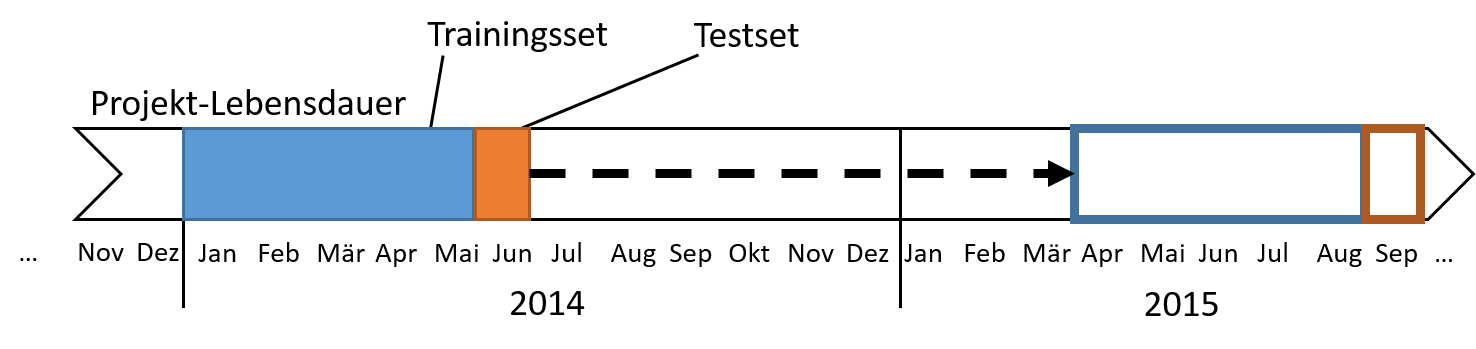
\includegraphics[width=1\textwidth]{resources/images/sliding_window_experiment.png}
	\caption[Visualisierung eines Sliding-Window-Experiments]{Das Sliding Window, bestehend aus Trainings- und Testset, wird über die Projekt-Lebensdauer geschoben.}
	\label{fig:sliding_window}
\end{figure}



% Mehr Testen
%% Gemäss unserem ursprünglichen Plan
%% Vielleicht automatisieren
%% Mehr Features
%% Feature-Selection


\subsubsection{Vision einer einsetzbaren Lösung}

Falls sich die Methoden dieser Arbeit in Zukunft zur Fehlervorhersage mit realen Projekten als tauglich erweisen, wäre eine denkbare Anwendung das Bestimmen einer ``Heatmap'' für Softwareprojekte. Eine solche würde anzeigen, welche Komponenten besonders fehleranfällig sind, was sowohl Entwicklern als auch Projektleitern helfen könnte. 

Ein langfristiges Ziel könnte neben der Fehlervorsage auch die Fehlerlokalisierung sein. Dazu müsste allerdings die Granularität der Analyse verfeinert werden. Im Moment ist die kleinste Einheit eine Source-Code-Datei, d. h. in der Regel genau eine Java-Klasse. Für eine brauchbare Fehlerbestimmung müsste auf Methodenebene gearbeitet werden.

Eine produktiv eingesetzte Lösung sollte idealerweise auch weitere Programmiersprachen unterstützen. Die Integration der Sprache \emph{Boa}, welche bereits Unterstützung für verschiedene Programmiersprachen bietet, könnte bei diesem Unterfangen sehr hilfreich sein. Damit die unterschiedlichen Programmiersprachen identisch verarbeitet werden können, wäre eine Zwischensprache notwendig. Neben der Definition dieser Zwischensprache ist auch ein Tool zur Übersetzung des Source Codes in einen \ac{AST} notwendig.

Damit die in unserer Arbeit entwickelten Tools ihrer Arbeit nachgehen kön\-nen, ist eine Menge an Konfiguration nötig. Zudem müssen sie der Reihe nach einzeln gestartet werden. Um später ein schlüsselfertiges Tool zur Verfügung zu stellen, sollten diese Einschränkungen aufgehoben werden.

Eine Idee ist, den Dienst direkt aus der Cloud als Service anzubieten, wie es zum Beispiel Code Climate \cite{codeclimate} tut. Die Software sollte per Self-Service an die vom Programmierer verwendete Versionsverwaltung angebunden werden. Die Fehlervorsage könnte per Webhooks \cite{githubwebhooks} sogar automatisch bei jedem Commit ausgelöst werden. Damit könnte der Qualitätsstand des Projektes quasi ``live'' mitverfolgt werden.

Natürlich ist das nur ein Beispiel von vielen Möglichkeiten, eine \ac{ML}-gestützte Fehlervorhersage für Source Code einzusetzen. Auf jeden Fall ist es noch ein weiter Weg, bis eine produktiv nutzbare Lösung realisierbar ist. Wir glauben aber, dass es sich lohnt, diesen zu beschreiten.

\section{Verzeichnisse}
%\subsection{Literaturverzeichnis}
\nocite{*}
\printbibliography[heading=subbibnumbered]

\lstlistoflistings

%\subsection{Abbildungsverzeichnis}
\listoffigures

%\subsection{Tabellenverzeichnis}
\listoftables

\subsection{Abkürzungsverzeichnis}
\begin{acronym}[]
	\acro{ML}{Machine Learning}
	\acro{UML}{Unified Modeling Language}
	\acro{SVN}{Subversion}
	\acro{CVS}{Concurrent Versions System}
	\acro{PaaS}{Platform as a Service}
	\acro{REST}{Representational State Transfer}
	\acro{API}{Application Programming Interface}
	\acro{DB}{Datenbank}
	\acro{DBMS}{Database Management System}
	\acro{SQL}{Structured Query Language}
	\acro{ORM}{Object Relational Mapping}
	\acro{AST}{Abstract Syntax Tree}
	\acro{MSR}{Mining Software Repositories}
	\acro{SVM}{Support Vector Machine}
	\acro{SVR}{Support Vector Regression}
	\acro{RBF}{Radial Basis Function}
	\acro{CV}{Cross Validation}
	\acro{MAE}{Mean Absolute Error}
	\acro{MSE}{Mean Squared Error}
	\acro{MDE}{Median Absolute Error}	
	\acro{PCA}{Principal Component Analysis}
\end{acronym}

\addcontentsline{toc}{section}{A Projektmanagement}
\addcontentsline{toc}{section}{B Installationsanleitungen}
\addcontentsline{toc}{section}{C Benutzeranleitungen}

\end{document}